\documentclass{scrartcl}

\usepackage[utf8]{inputenc} % use utf8 file encoding for TeX sources
\usepackage[T1]{fontenc}    % avoid garbled Unicode text in pdf
\usepackage[german]{babel}  % german hyphenation, quotes, etc
\usepackage{hyperref} % for pdf conversion (links etc.)
\usepackage{csquotes} % provides \enquote{} macro for "quotes"
\usepackage[nonumberlist]{glossaries}  % provides glossary commands
\usepackage{enumitem} % provide enumerate
\usepackage{float} % nötig für {table}[H]
\usepackage{graphicx}
\usepackage{geometry}
\usepackage{pdfpages}
\usepackage{placeins}


\hypersetup{
    pdftitle={Entwurfsheft},
}

%\makenoidxglossaries
%\input{glossary}


\title{Entwurf\\
		MatFlow \\
        Workflowanwendung für Machine Learning Experimente}
\author{Florian Küfner, Soeren Raymond, Alessandro Santospirito, \\ 
        Lukas Wilhelm, Nils Wolters} 
\date{Dezember 2021}

\begin{document}
\newcommand{\class}[1]{\begin{center}\Large\bfseries Class: #1 \end{center}}
\newcommand{\method}[1]{\item \textbf{#1}}
\newenvironment{methodenv}[1]{\paragraph{#1}\begin{itemize}}{\end{itemize}}
\newcommand{\smallPara}[1]{\subparagraph{\small #1}}

\newenvironment{dataTable}{\begin{tabular}{|p{4cm}|p{2cm}|p{6cm}|}}{\end{tabular}}


% Titel
\maketitle
\pagebreak
\setcounter{tocdepth}{2} 
\tableofcontents
\pagebreak

% Inhalt
 

\section{Einleitung}

% schreiben wir am Ende

\newpage
\input{systemüberblick}
\section{Kommunikation}

\subsection{Client $\leftrightarrow$ Server} 
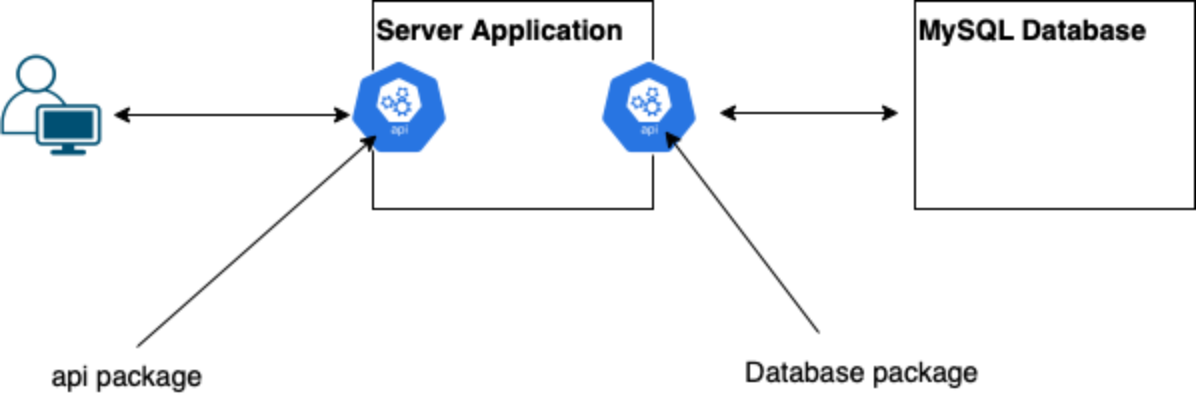
\includegraphics[width=1\textwidth]{res/Kommunikation.png}
Die Kommunikation zwischen Client und Server erfolgt über das \nameref{API}, bei der die Klasse FrontendAPI 
als RESTful API über JSON mit dem Client kommuniziert und das Database Package die Kommunikation 
zwischen der Datenbank und der Server Application regelt. Beide Schnittstellen sind zugleich Fassaden, die die Kommunikation
zwischen den einzelnen Subsystemen regeln.
Hier ist also eine horizontale Schichtenarchitektur vorhanden.

%Frontend API
\subsubsection{Frontend API}
Hinweis: Json Objekte werden in Python nativ als String interpretiert. Das ist dementsprechend im Entwurf aber durch die 
Benennung der Parameter klar, da json Objekte immer mit json\texttt{\_}details o.Ä. beschrieben werden. \\ \\
Mithilfe von Flask läuft auf dem Hostserver eine RESTful API, von der ein Status Code geholt werden kann, der über den Erfolg 
bzw. über den Art des geworfenen Fehlers Auskunft gibt.\\ 
Da wir uns hier mit Fehlern der MatFlow Anwendung auseinandersetzen, sind alle Fehler im 6xx Format.
Folgende spezifische Fehlerarten gibt es, d.h. diese Status Codes erweitern die standardisierten Codes wie etwa 404:
\begin{itemize}
    \item 601: UserExistsException
    \item 602: DoubleTemplateNameException
    \item 603: InvalidDagFileException
    \item 604: DoubleWorkflowInstanceNameException
    \item 605: EmptyConfigFolderException
    \item 606: WorkflowInstanceRunningException
    \item 607: successful Operation
\end{itemize}

%Lukas zum Database package
\subsubsection{Database package}
Die Kommunikation zwischen BackEnd und MySQL-Server läuft allein durch die Klasse DatabaseTable des Pakets \nameref{database}. 
Der Verbindungsaufbau ist mit der Pythonbibliothek MySQLdb vorgesehen.


\subsection{Server $\leftrightarrow$ Airflow API}
Der Server kommuniziert mit Airflow über die Airflow API, um die Benutzerrollen Reviewer, Developer und Administrator zu erstellen.
Außerdem wird die Airflow API dazu benötigt, Benutzer zu registrieren und zu bearbeiten.
Des Weiteren wird die Airflow API dazu benutzt um herauszufinden ob ein bestimmter Workflow gerade ausgeführt wird.

\newpage
\subsection{Entwurfsmuster}

\subsubsection{MatFlow}
MatFlow, wie schon im Kommunikationskapitel gesehen, ist eine Schichtenarchitektur, die über Fassaden miteinander verbunden ist
(\nameref{API} und Database package). Im größeren Bild ist die gesamte Software aber eine Rahmenarchitektur, da MatFlow
durch Plugins Apache Airflow erweitert.

\subsubsection{\nameref{API}}
Hier ist die Klasse FrontendAPI die eigentliche Fassade. Der Grund dafür ist womögliche Abhängigkeiten zwischen
der Client Applikation und der Serverapplikation zu entkoppeln. Sie wurde als Singleton implementiert, da die API
nur auf einem Port auf dem Server laufen soll und global ansprechbar sein soll. Mehrere essentiell gleiche APIs auf
verschiedenen Ports wären uneindeutig.


\newpage
\section{Komponentenbeschreibung}

\subsection{Client}
Das Frontend besitzt das Design-Muster View-Model-Controler als übergeordnetes Muster. Im Packet \glqq View\grqq{} befinden sich die mit HTML und CSS designten Webseiten. Das Packet \glqq Model\grqq{} dient als Bindeglied zwischen dem \glqq View\grqq{}-Packet und dem \glqq Controller\grqq{}-Paket. Es beinhaltet die Daten die in den Aufbau einer Webseite eingebunden werden und fragt diese an und lässt sie ändern im Packet \glqq Controller\grqq{}. Einen austausch zwischen dem Frontend und dem Backendserver erfolgt im Packet \glqq Controller\grqq{}. Dies beinhaltet die Daten-, Lösch und Änderungsanfragen.

\begin{figure}[H]
\centerline{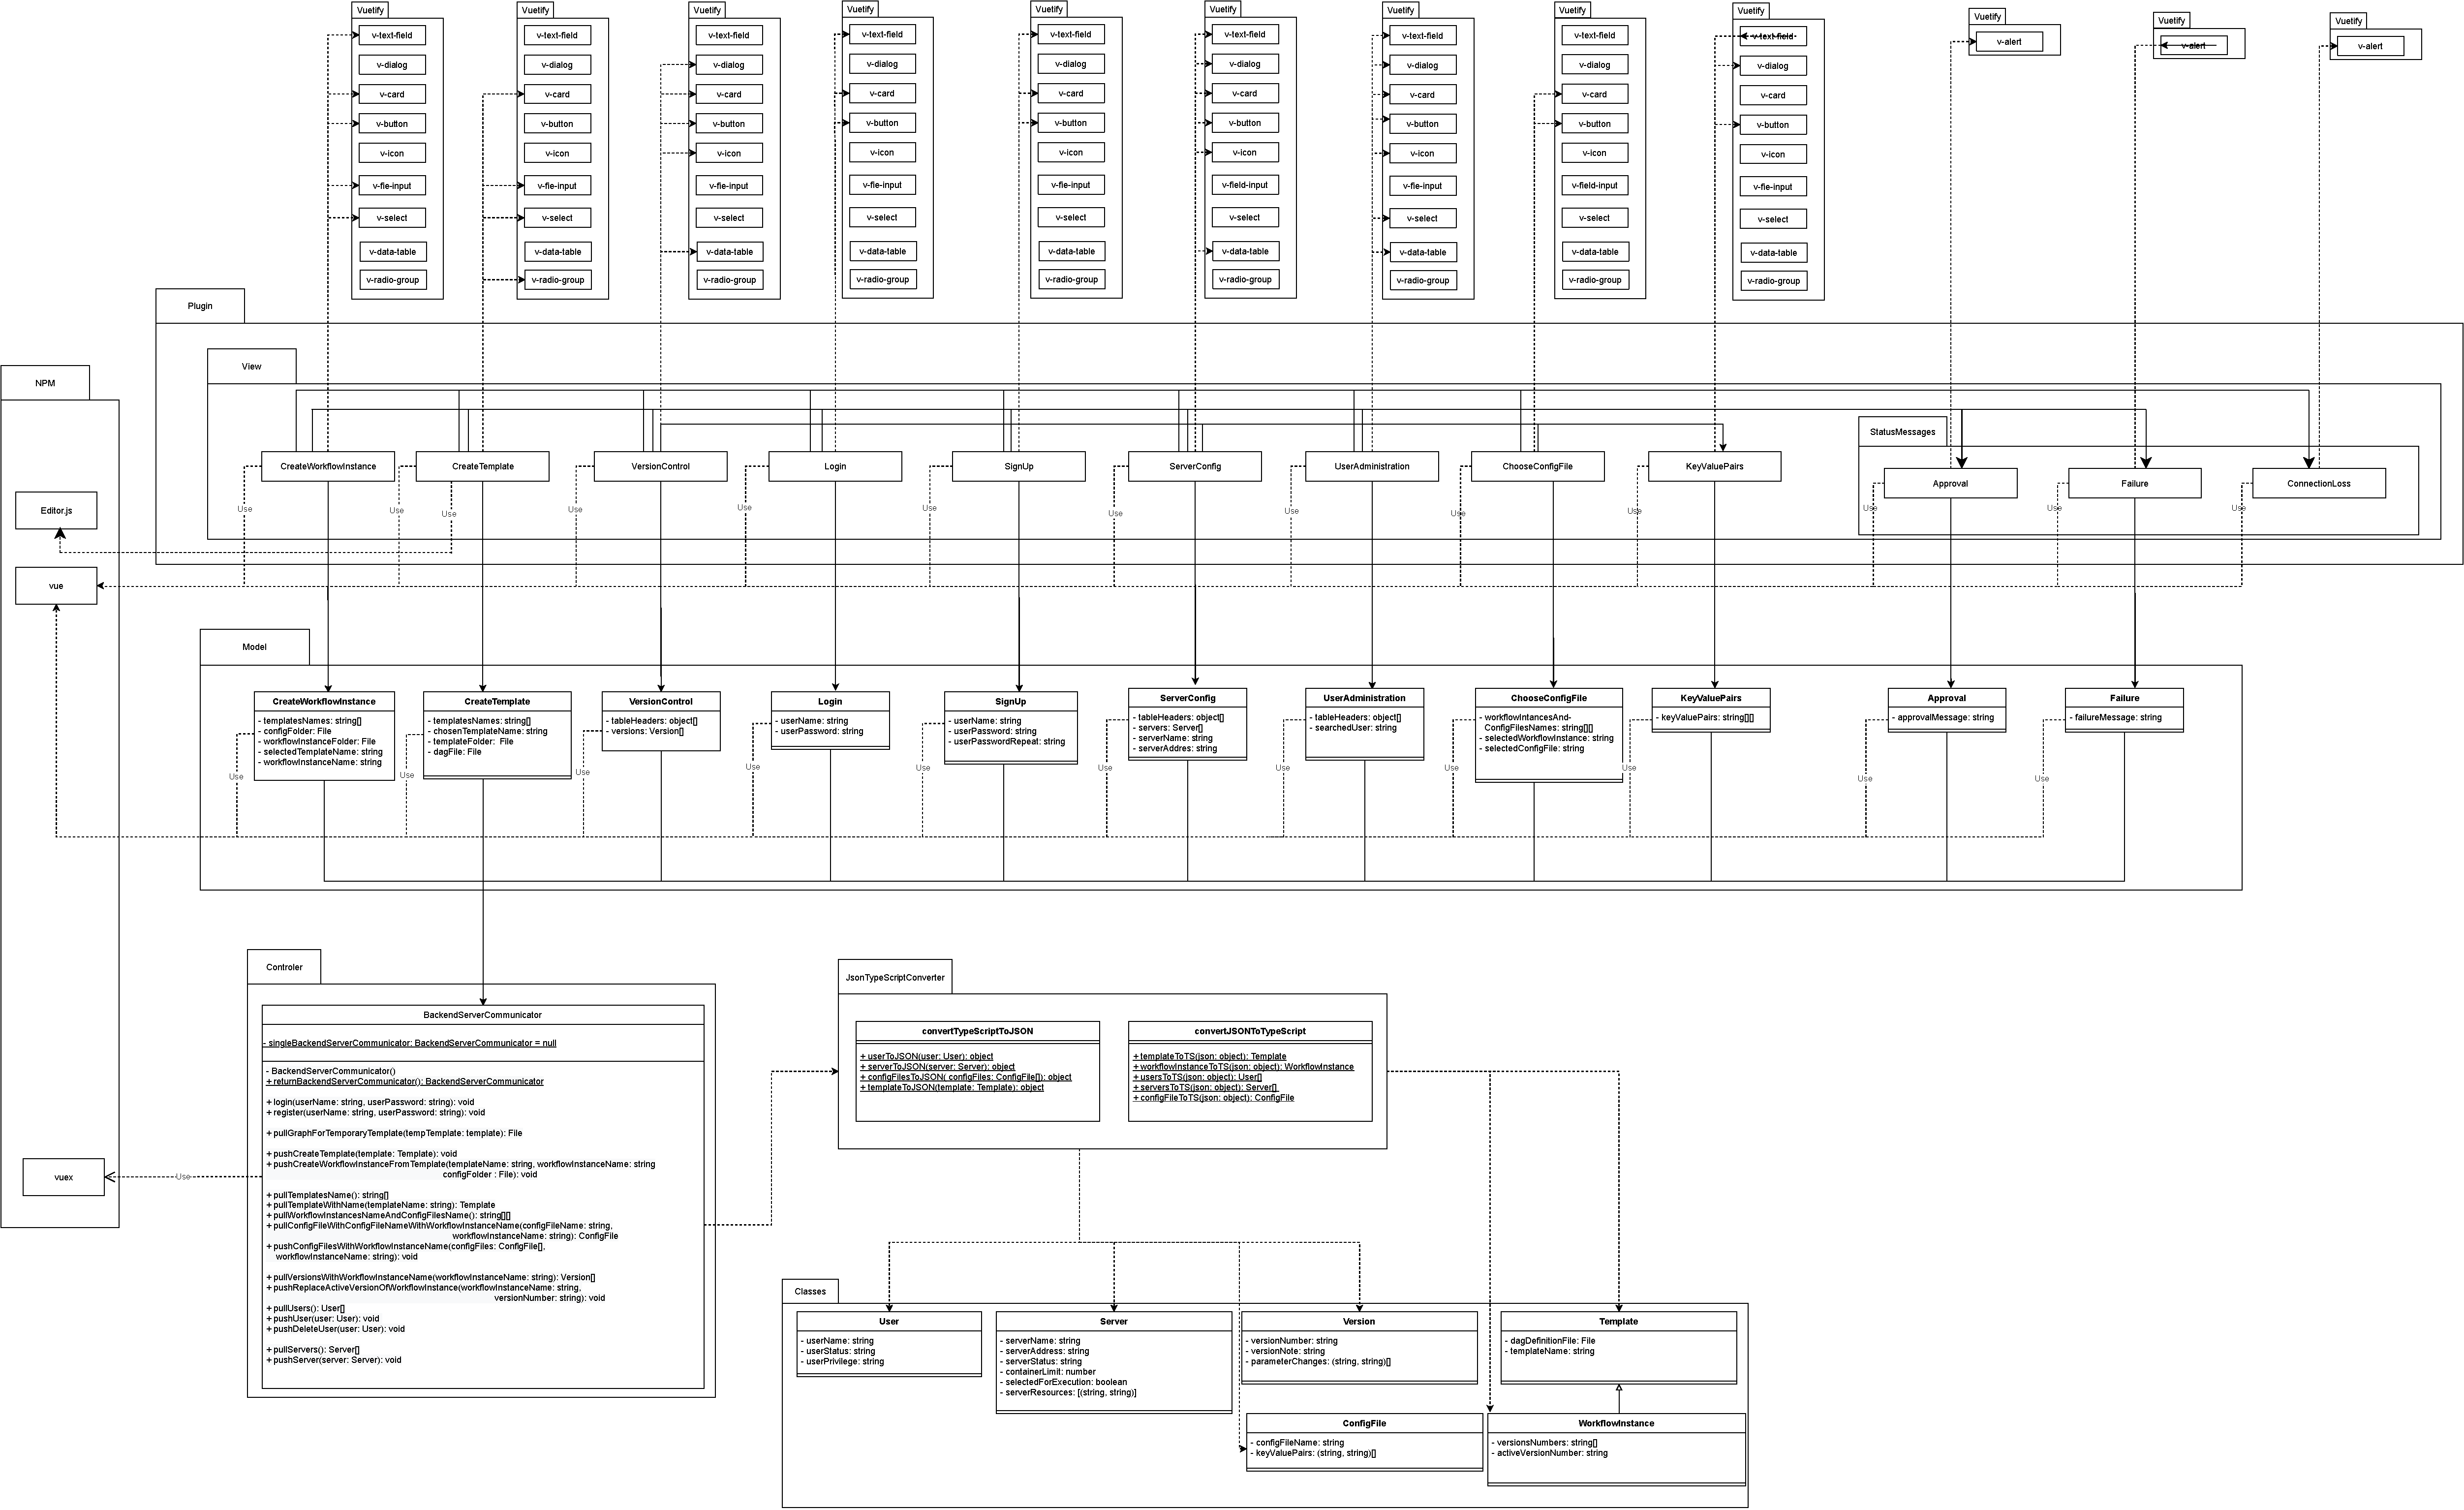
\includegraphics[scale=0.2]{res/FrontendUML.drawio.pdf}}
\caption{Klassendiagramm zum Frontend}
\end{figure}

\newpage

\subsection{Server}

\subsubsection{Überblick}
\begin{figure}[H]
    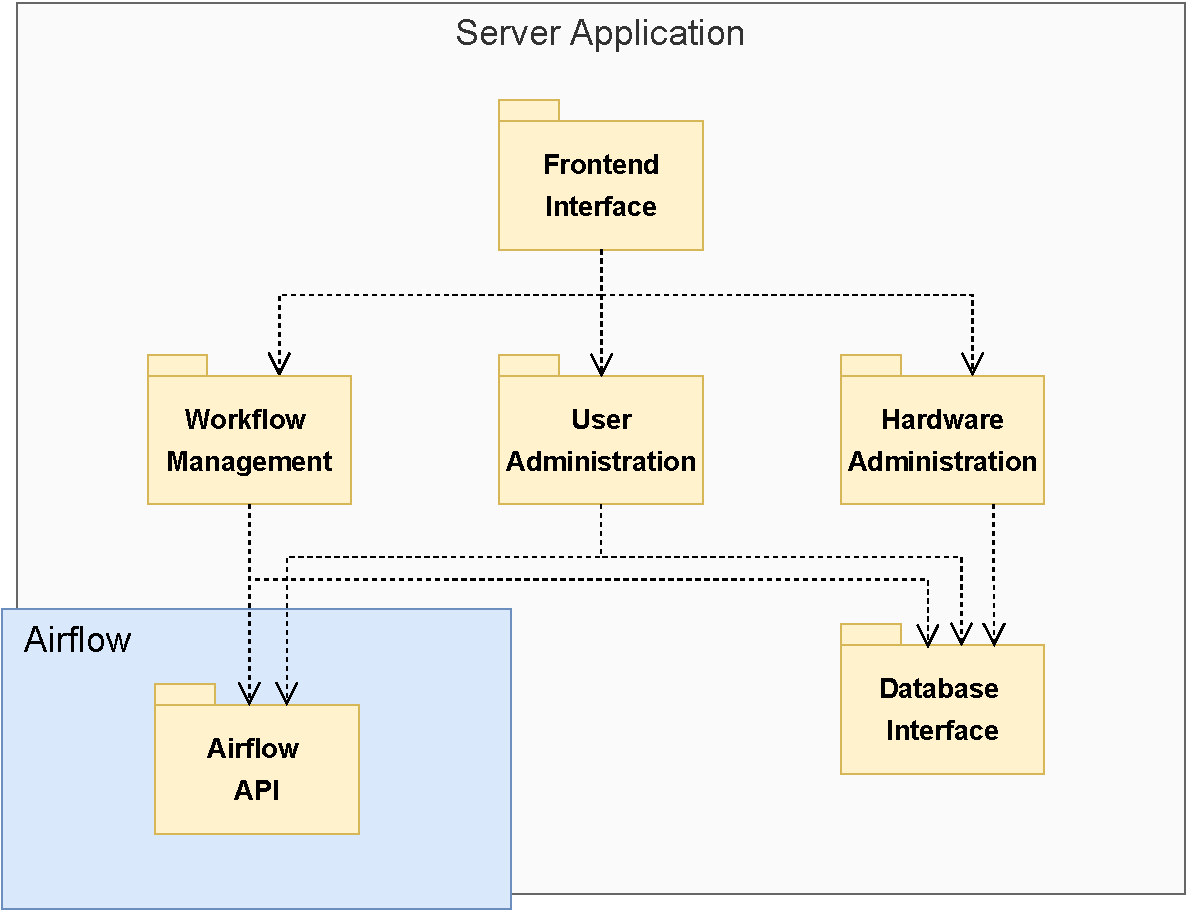
\includegraphics[width=1\textwidth]{res/Moduluebersicht.pdf}
    \caption{Übersicht über den Entwurf der Server Anwendung}
\end{figure}
Die Server Anwendung ist in ihren Grundzügen in einer Schichtenarchitektur aufgebaut. 
Die zentrale Anlaufstelle für Anfragen des Clients stellt das API Package dar.
Dieses hat Abhängigkeiten zu den Workflow, User Administration und Hardware Administration Packages, welche wiederum auf die Datenbank-Schnittstelle und die Airflow API zugreifen.


\subsubsection{\nameref{API}}
\begin{figure}[H]
    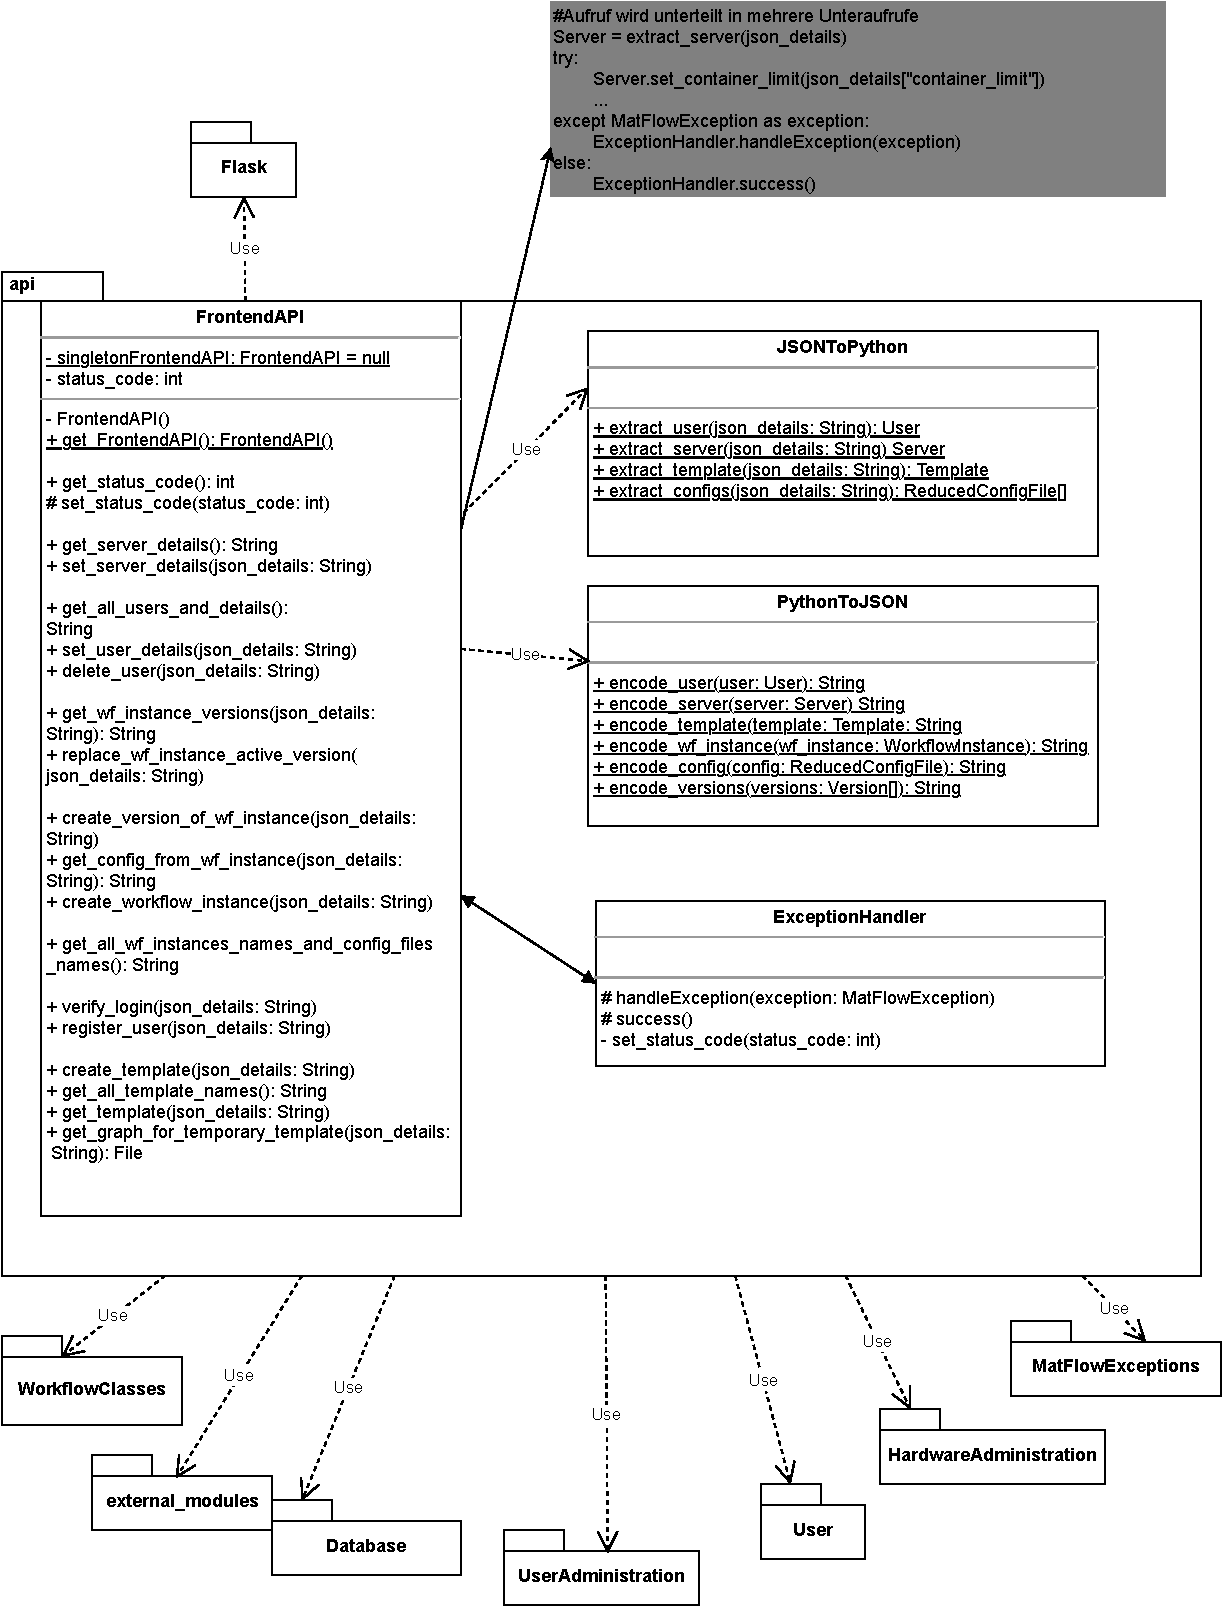
\includegraphics[width=1\textwidth]{res/api.drawio.pdf}
    \caption{API Package}
\end{figure}
Dieses Package ist zuständig für die Kommunikation zwischen der Client Applikation und der Serverapplikation (siehe Kapitel 
Kommunikation). Anfragen an die Klasse FrontendAPI werden an die dementsprechenden packages weitergeleitet, wo diese konkret 
ausgeführt werden. Diese Klasse fängt alle Exceptions und leitet sie an die Klasse ExceptionHandler weiter.
In der ExceptionHandler Klasse wird dann der Status Code der FrontendAPI Klasse geändert, der für den Client aussagekräftig
darüber ist welcher Fehler geworfen wurde.


\subsubsection{Workflow package}
\begin{figure}[H]
    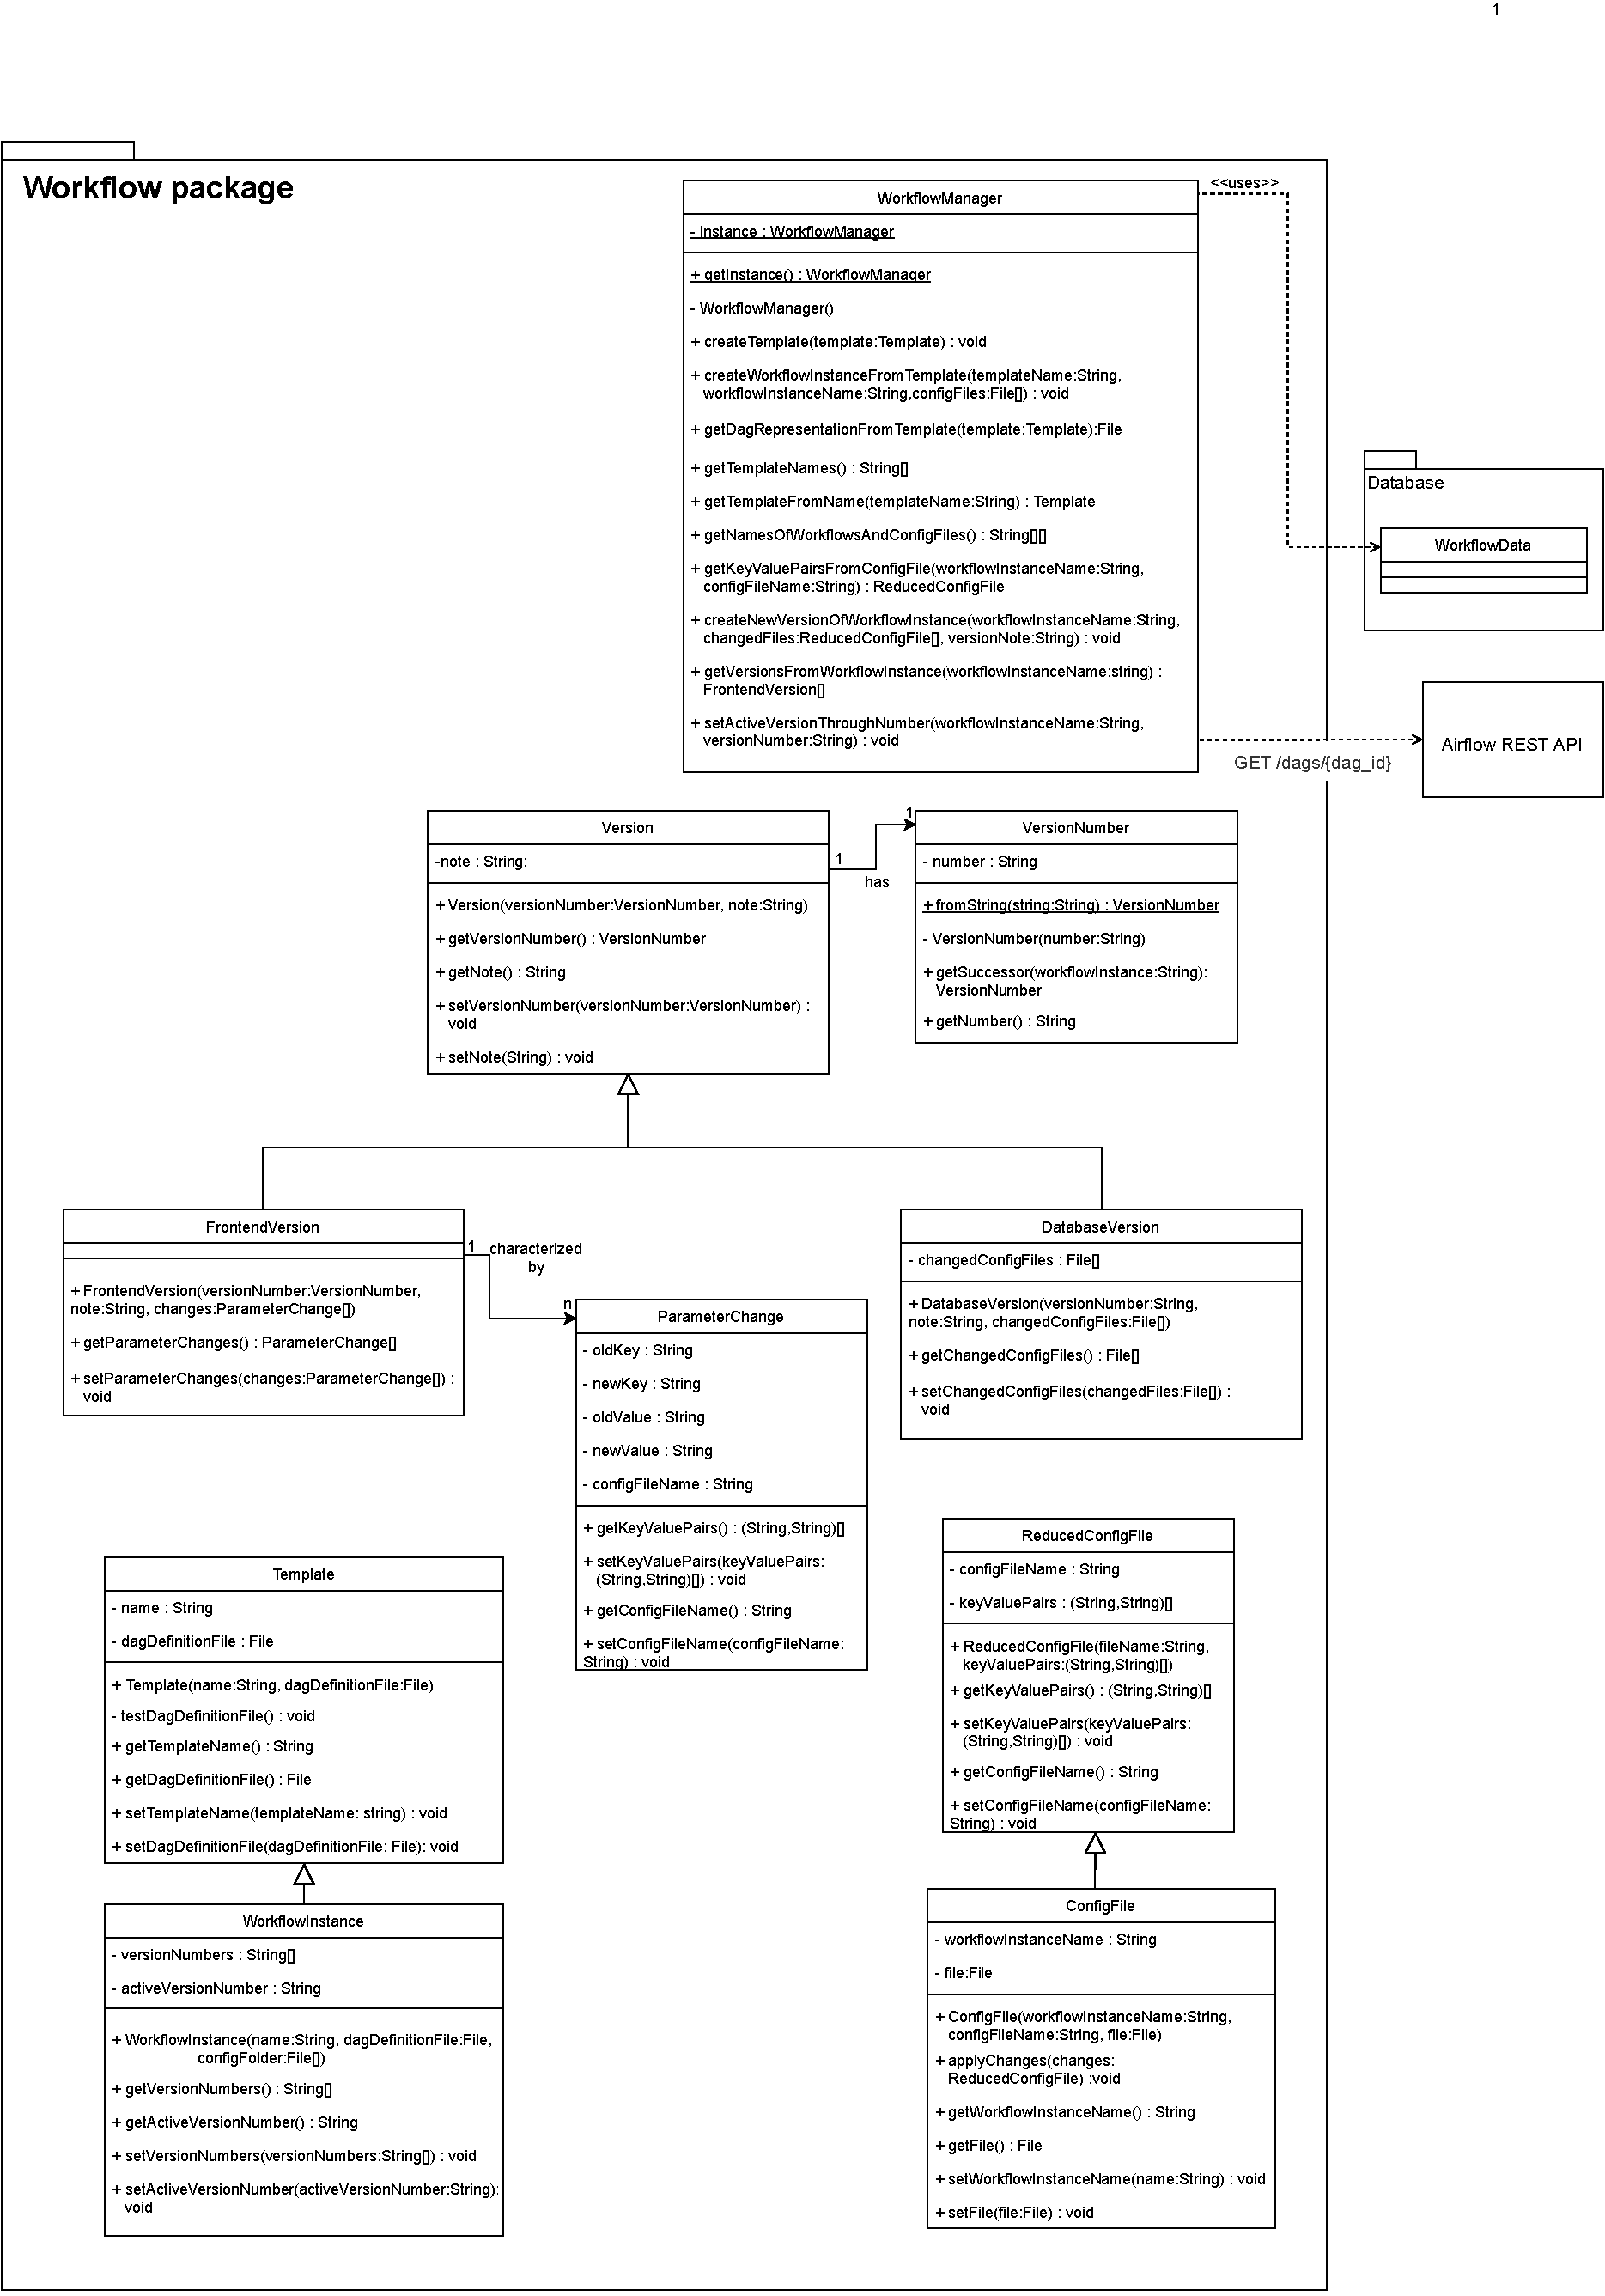
\includegraphics[width=1\textwidth]{res/Klassen/wfPackage.pdf}
    \caption{Klassendiagramm des Workflow packages}
\end{figure}
Das Workflow Package ist für die Erstellung und Verwaltung von Workflow-Templates, -Instanzen und -Versionen zuständig.
Es stellt ein Bindeglied in der Kommunikationskette zwischen Client, Airflow und der Datenban dar.
Alle Anfragen die vom Client gestellt und der API weitergeleitet werden kommen zentral im Singleton-Objekt der Klasse WorkflowManager an.
Dieses erstellt dann andere Objekte und stellt seinerseits Anfragen an die Airflow API und die Datenbank-Schnittstelle.

\subsubsection{User Administration}
\begin{figure}[H]
    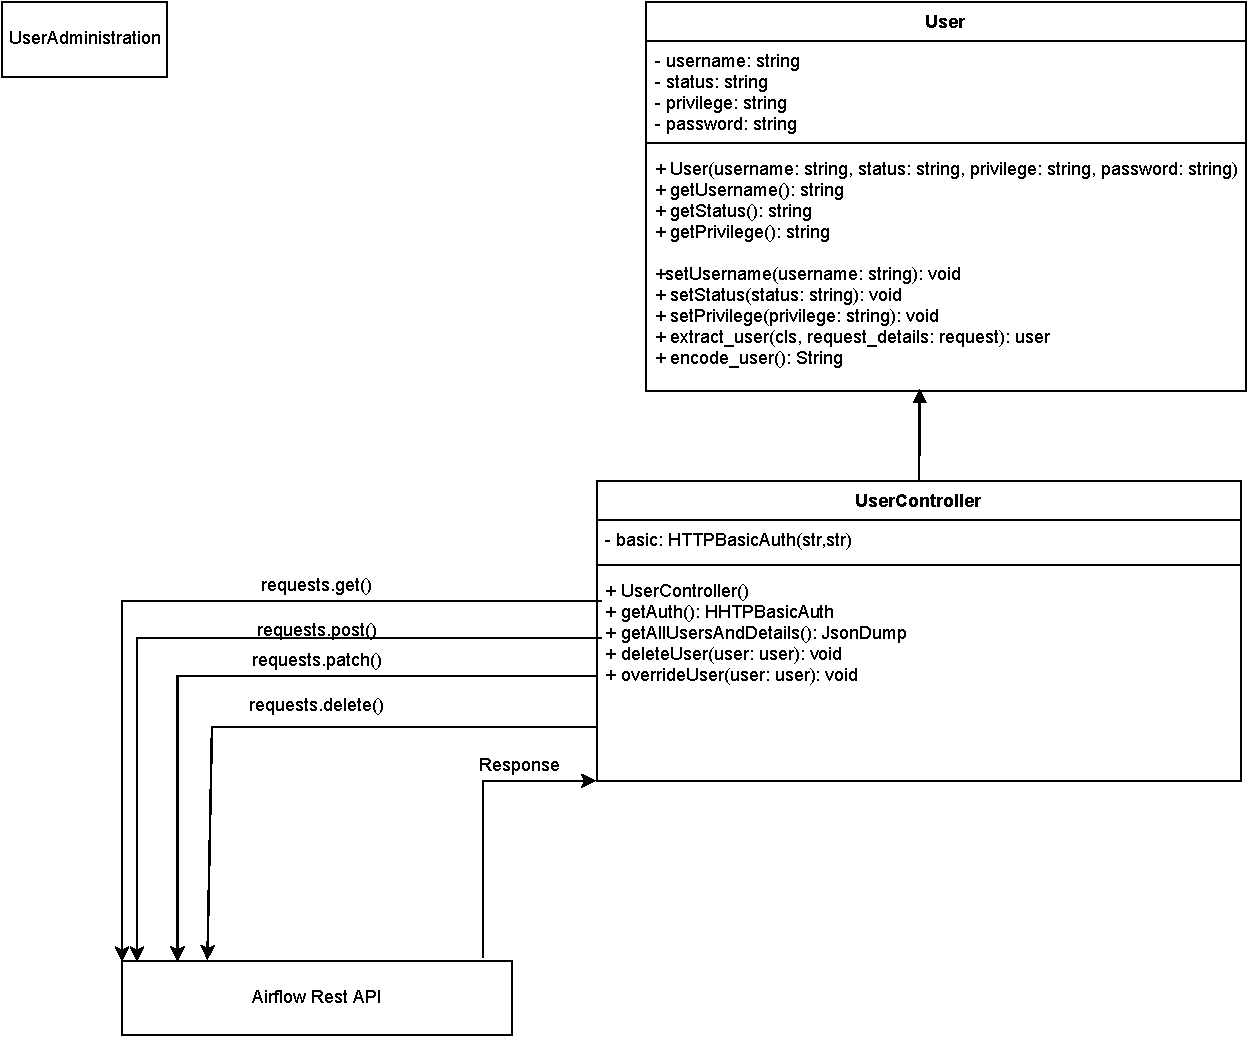
\includegraphics[width=1\textwidth]{res/UserAdministration.pdf}
    \caption{TODO Nils}
\end{figure}
TODO Nils

\subsubsection{Hardware Administration}
\begin{figure}[H]
    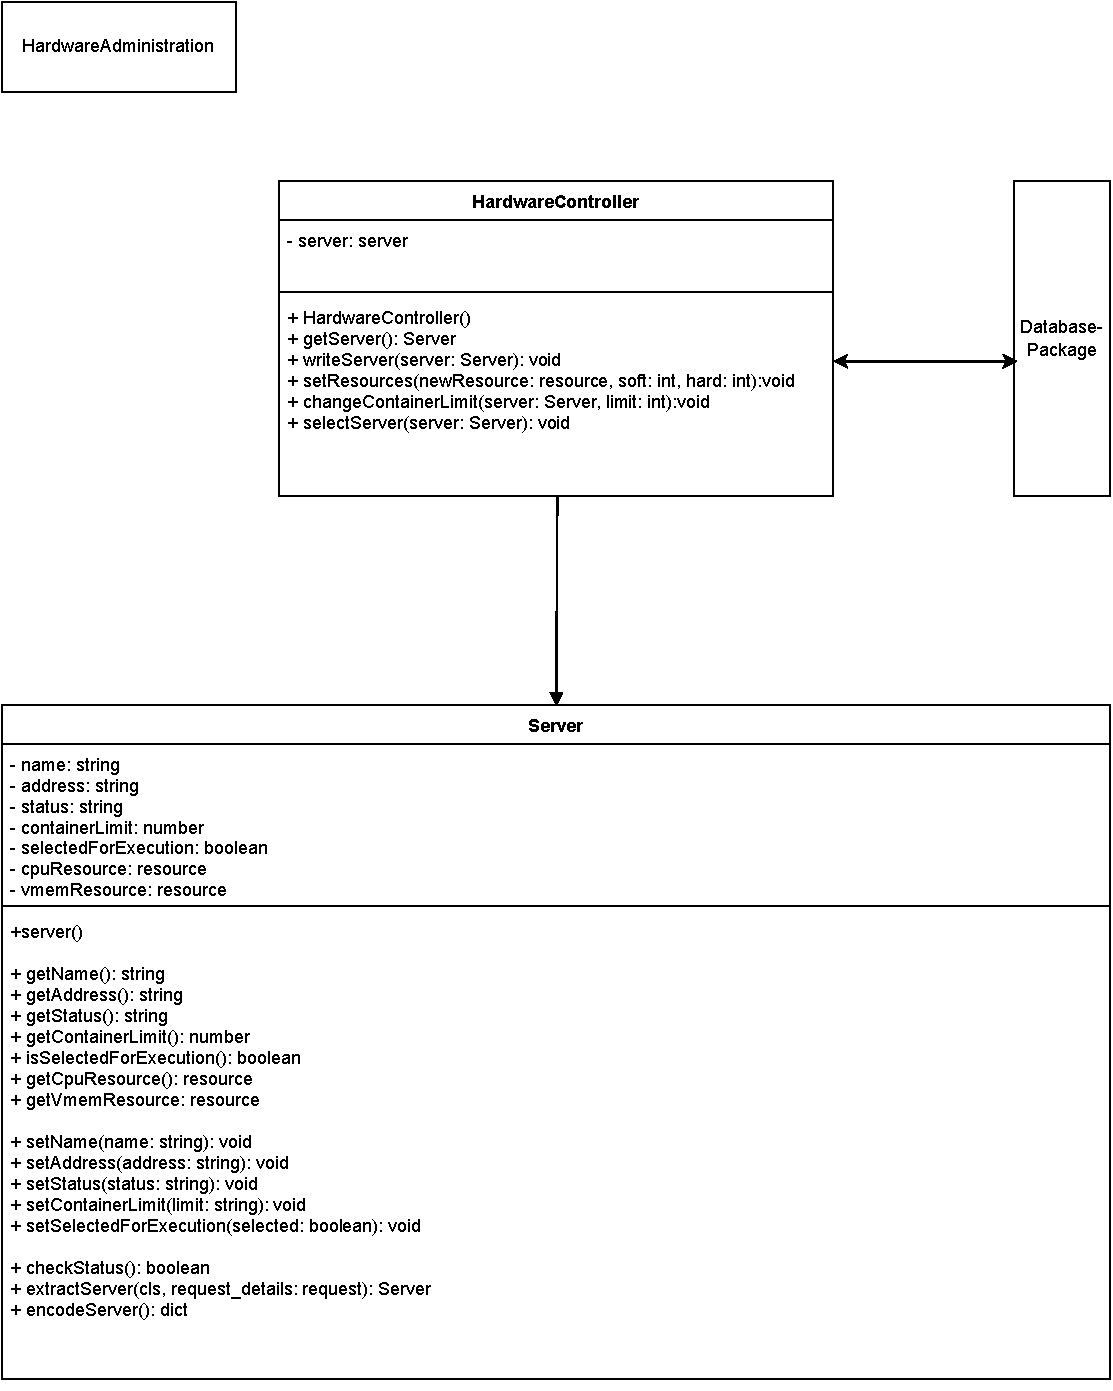
\includegraphics[width=1\textwidth]{res/HardwareAdministration.pdf}
    \caption{TODO Nils}
\end{figure}
TODO Nils

\subsubsection{\nameref{database}}
Entwirft für einen Aufruf einer Funktion einer Klasse in diesem Package den entsprechenden SQL Ausdruck und ruft diesen auf der Datenbank auf.
Bei fehlerhaften Aufrufen, wie zum Beispiel der Abfrage eines Workflows der nicht existiert, wird eine entsprechende MathFlowException an den Aufrufer zurückgeworfen.
\begin{figure}[H]
	\centering
	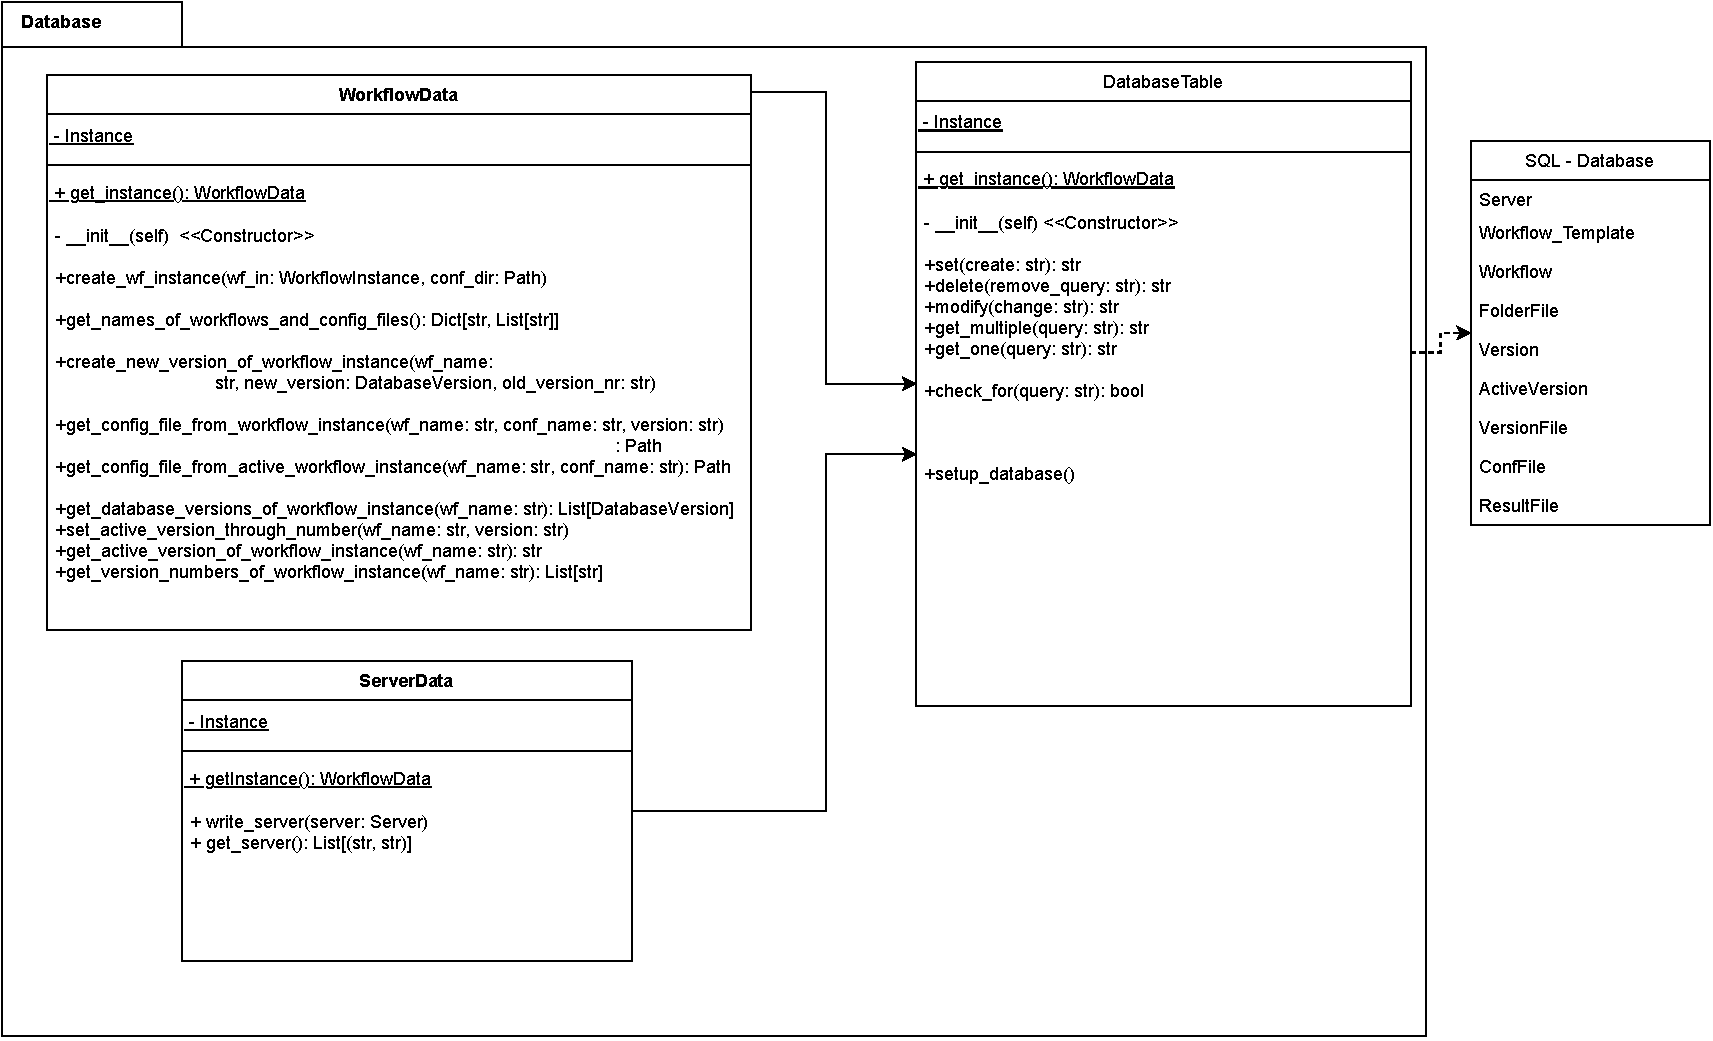
\includegraphics[width=1\textwidth]{res/Database_Package.pdf} 
	\caption{Klassendiagramm von Database}
	\label{fig:database_package}
\end{figure}


\subsubsection{TGDSOperator}
\begin{figure}[H]
    \centering
    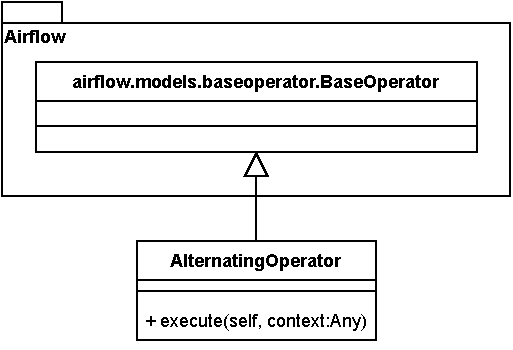
\includegraphics[width=0.65\textwidth]{res/Klassen/tgdsOp.pdf}
    \caption{Klassendiagramm des TGDS-Operators}
\end{figure}
Die Aufgabe dieses Packages ist es Airflow um einen weiteren Operator, den AlternatingOperator, zu erweitern.
Der Operator kann dann verwendet werden um zwei Tasks im Wechsel auszuführen. 
Dies ist bei der Implementierung eines bestimmten Theory-Guided-Data-Science-Modells von Nutzen. 


\subsubsection{MatFlowExceptions}
\begin{figure}[H]
    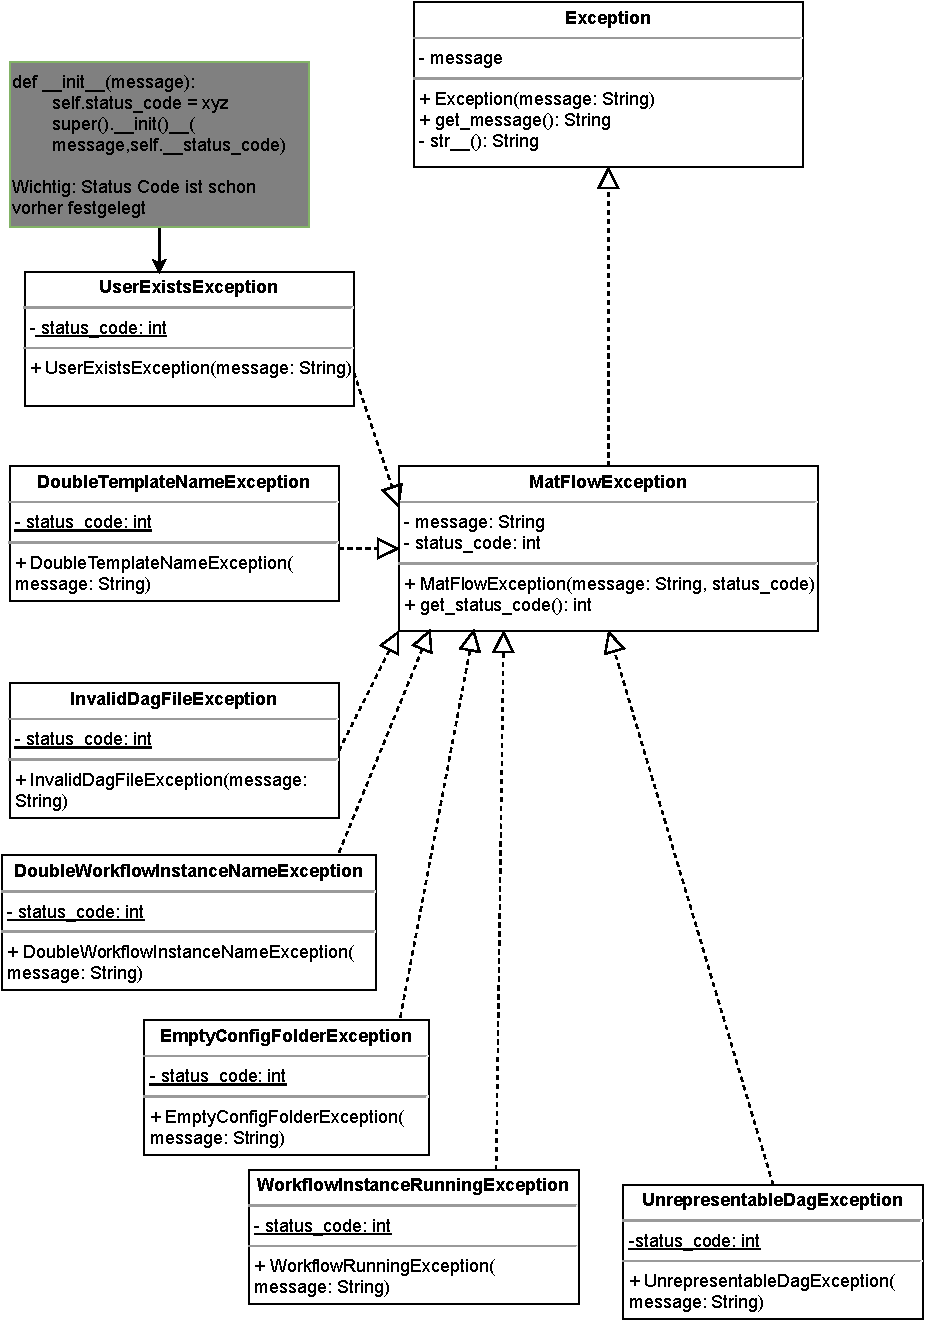
\includegraphics[width=1\textwidth]{res/Klassen/MatFlowExceptions.drawio.pdf}
    \caption{MatFlowExceptions}
\end{figure}
Dieses Package beinhaltet alle MatFlowExceptions. Diese werden geworfen, wenn es einen MatFlow spezifischen Fehler, ausgelöst 
durch den Nutzer, in der Anwendung gibt.


\newpage

\newpage
\section{Paketbeschreibung}
\subsection{Client Application}
\subsubsection{Model}
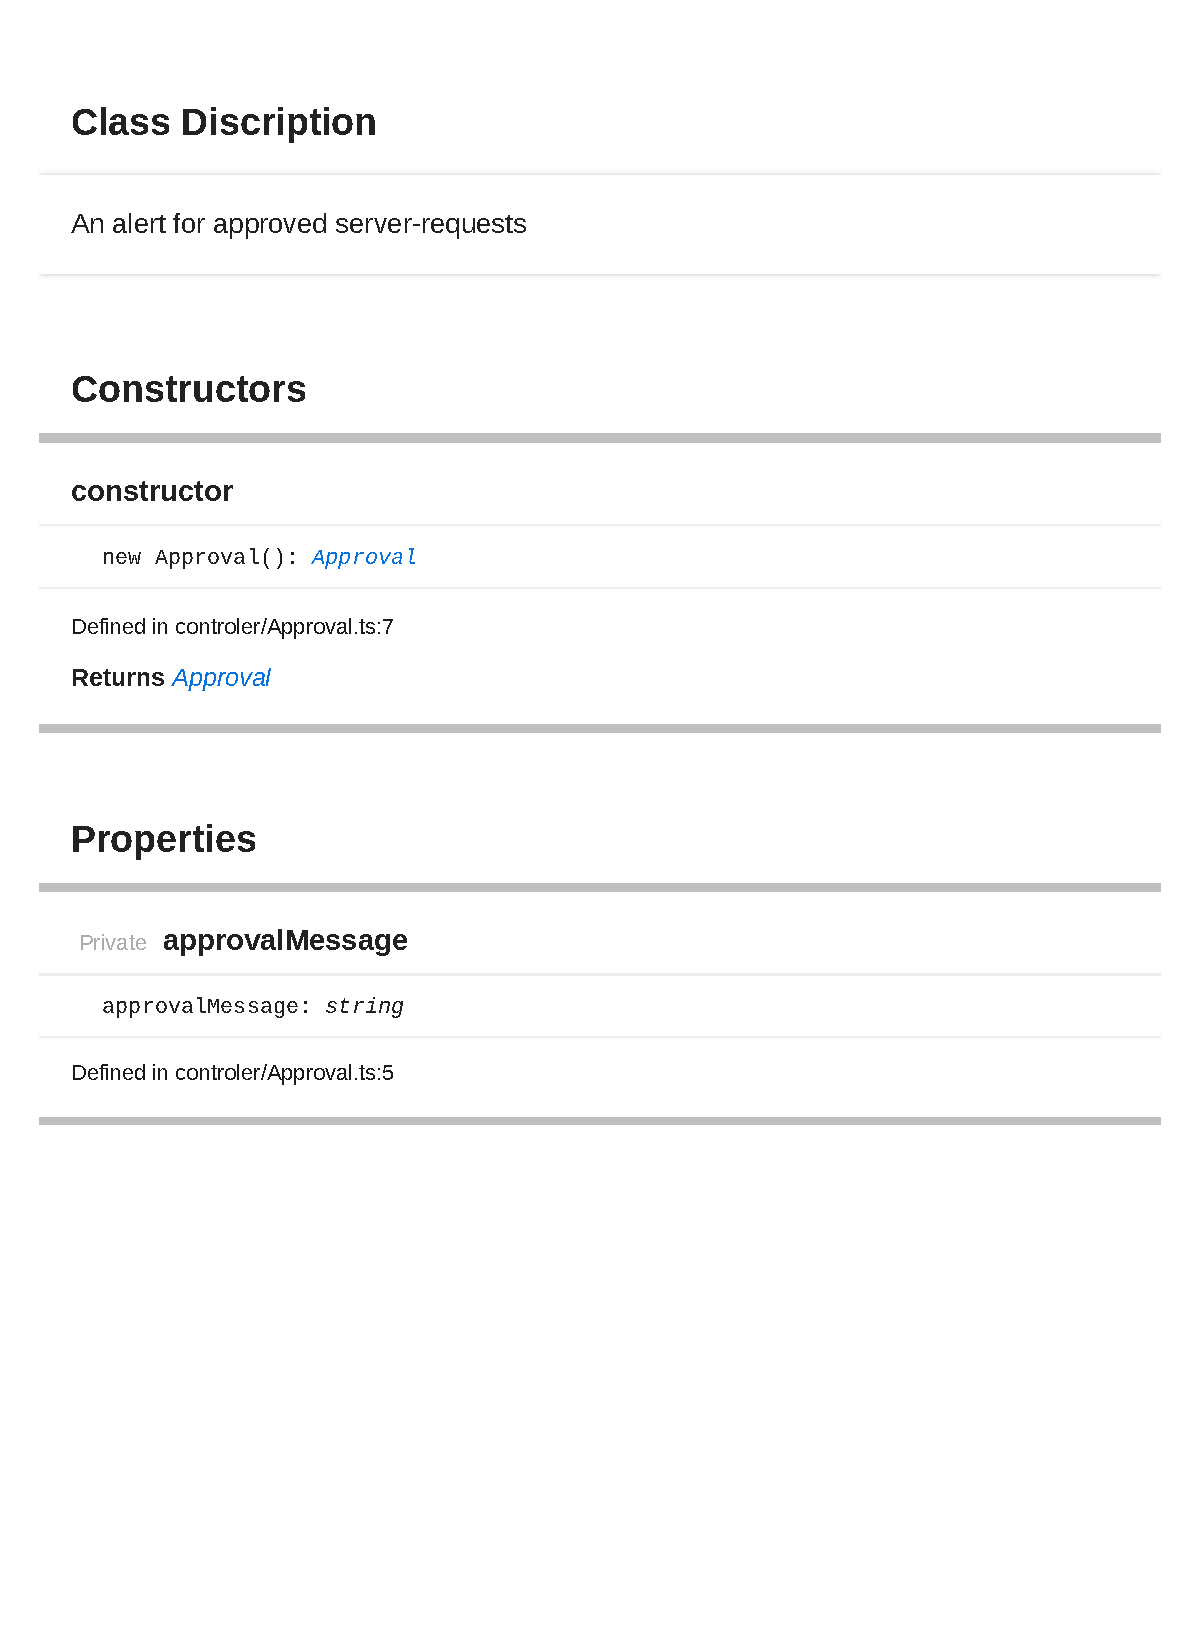
\includepdf[pages=1,  scale=0.8,pagecommand=\class{Approval}]{FrontendDocsAsPDF/Model/Approval.pdf}

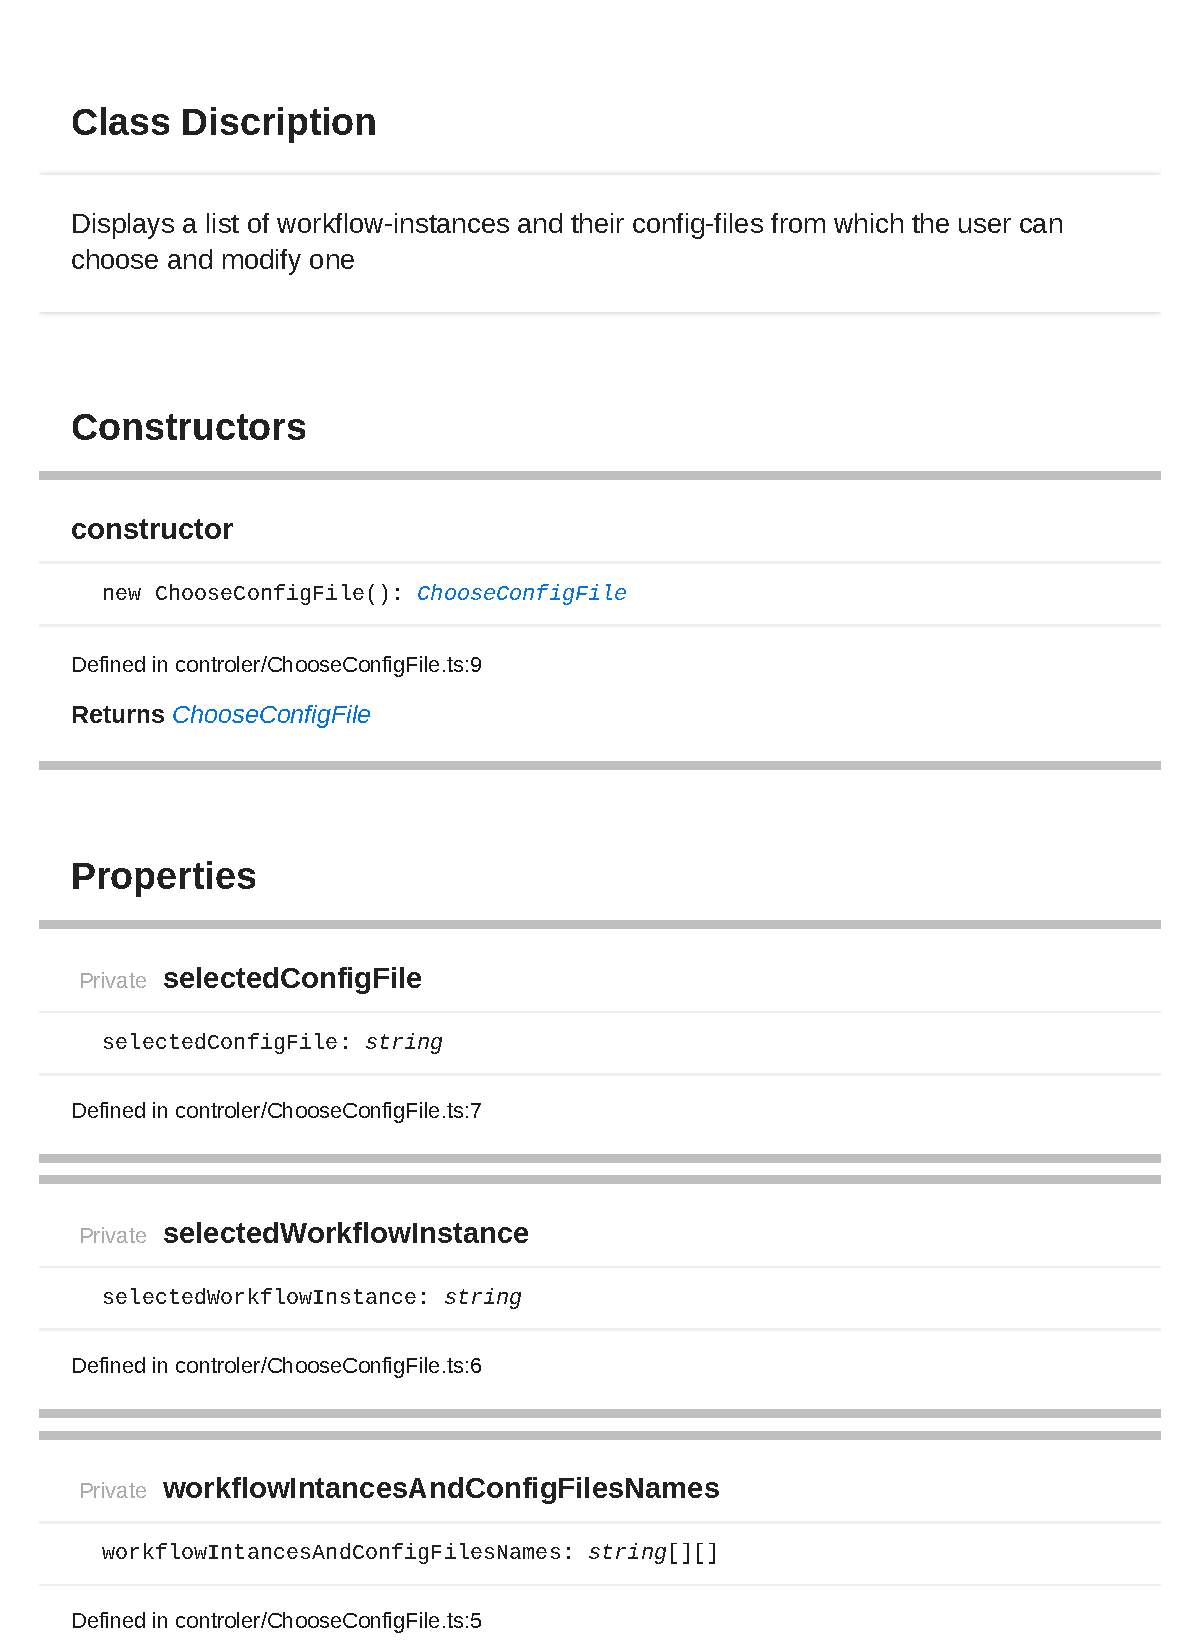
\includepdf[pages=1,  scale=0.8,pagecommand=\class{ChooseConfigFile}]{FrontendDocsAsPDF/Model/ChooseConfigFile.pdf}

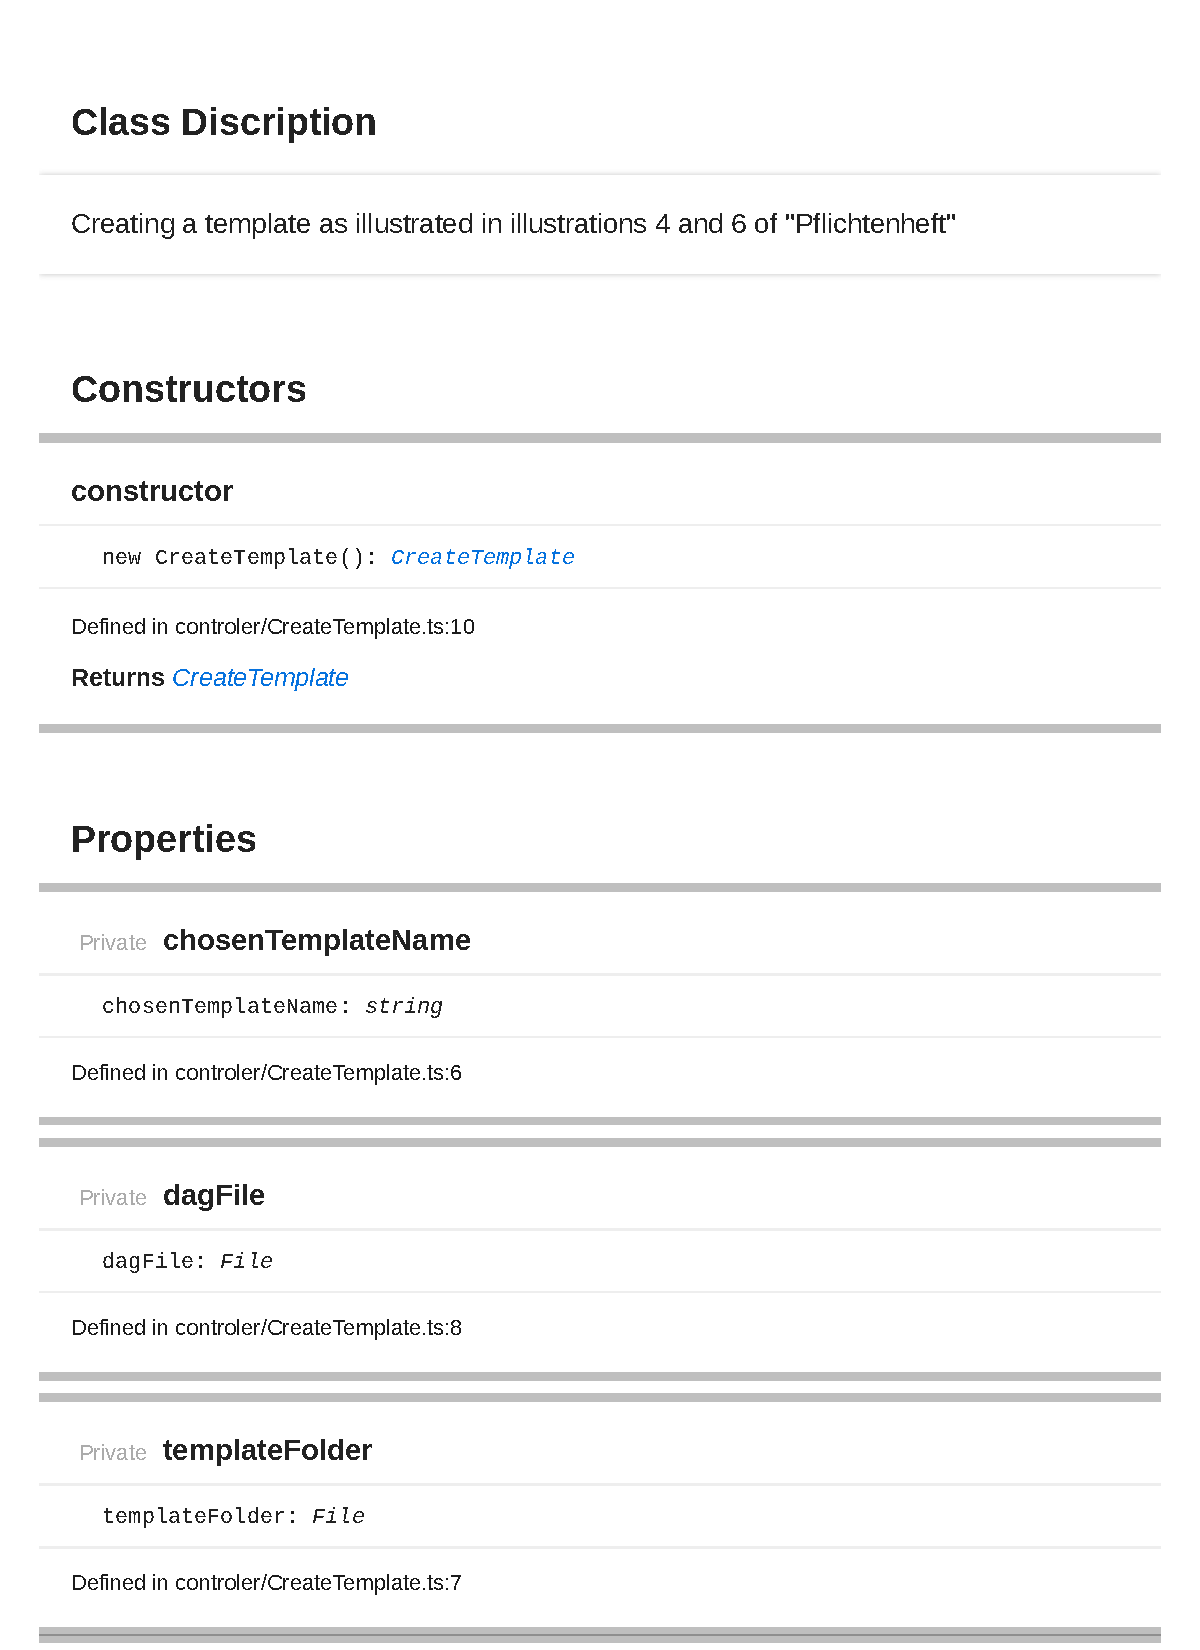
\includepdf[pages=1,  scale=0.8,pagecommand=\class{CreateTemplate}]{FrontendDocsAsPDF/Model/CreateTemplate.pdf}
\includepdf[pages=2-,  scale=0.8]{FrontendDocsAsPDF/Model/CreateTemplate.pdf}

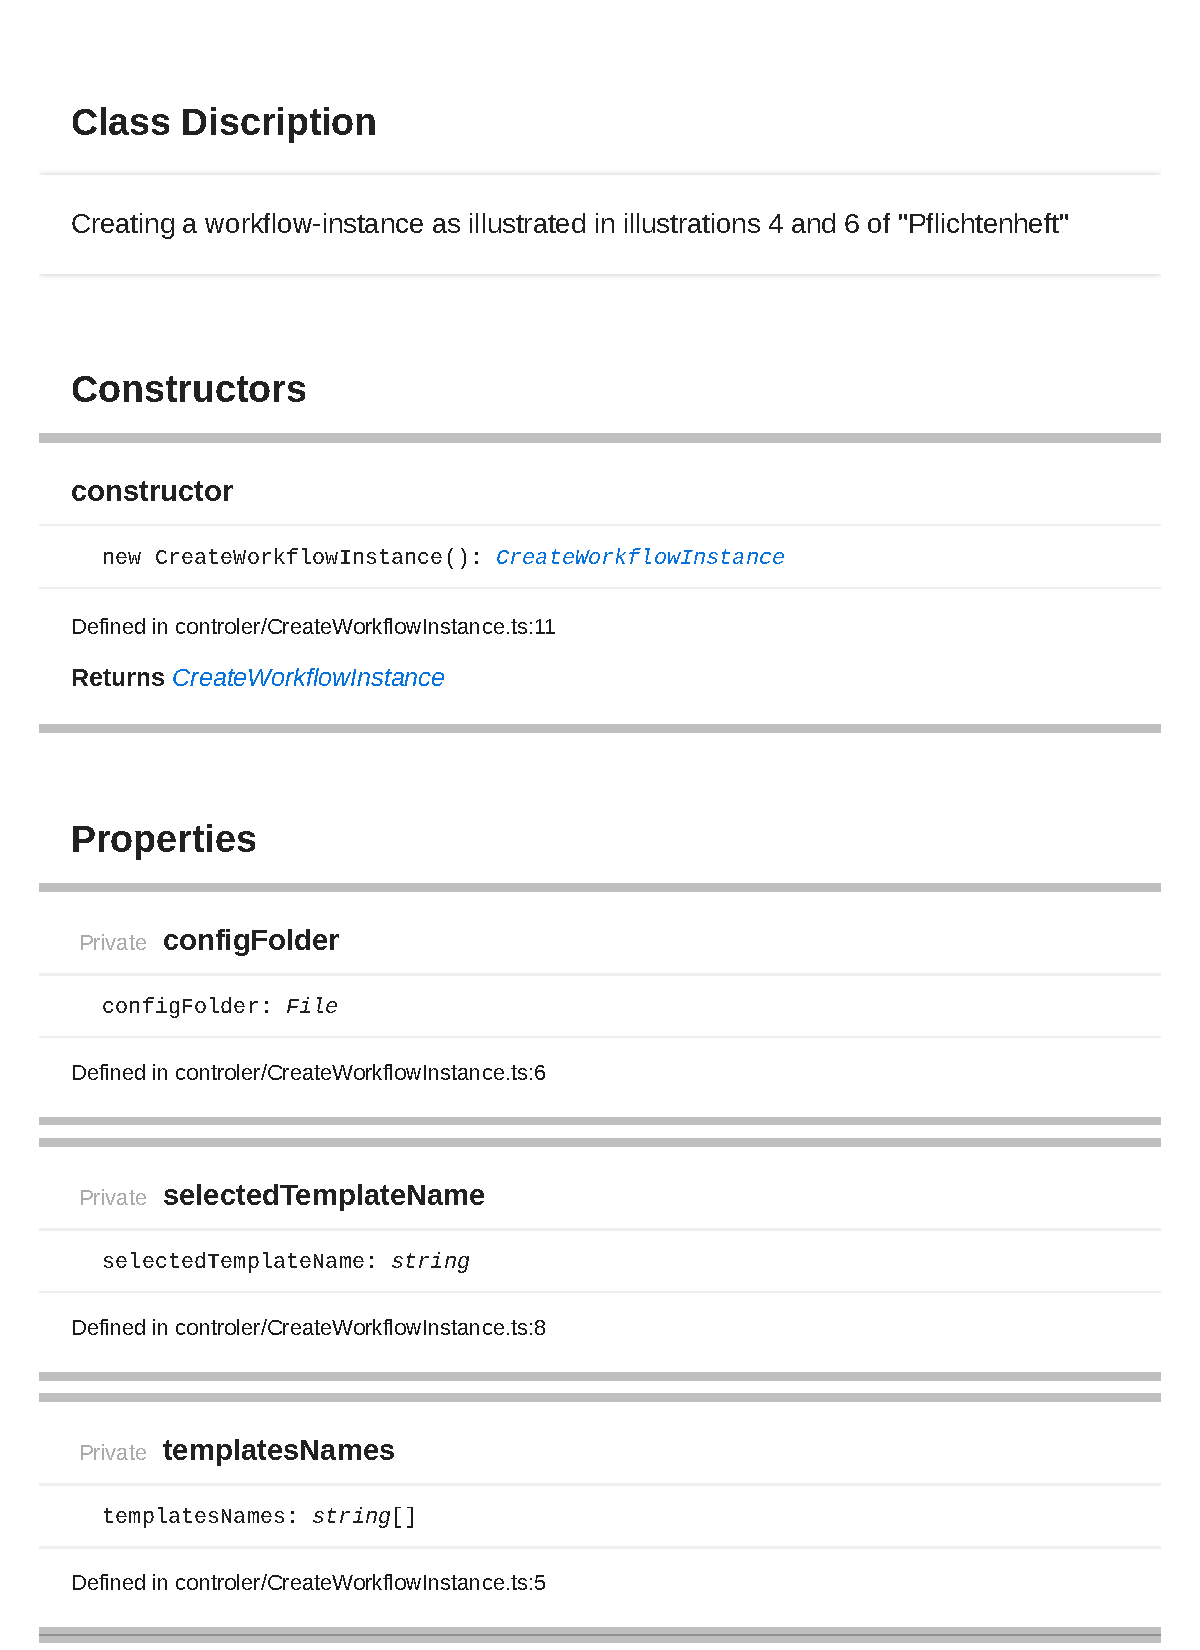
\includepdf[pages=1,  scale=0.8,pagecommand=\class{CreateWorkflowInstance}]{FrontendDocsAsPDF/Model/CreateWorkflowInstance.pdf}
\includepdf[pages=2-,  scale=0.8]{FrontendDocsAsPDF/Model/CreateWorkflowInstance.pdf}

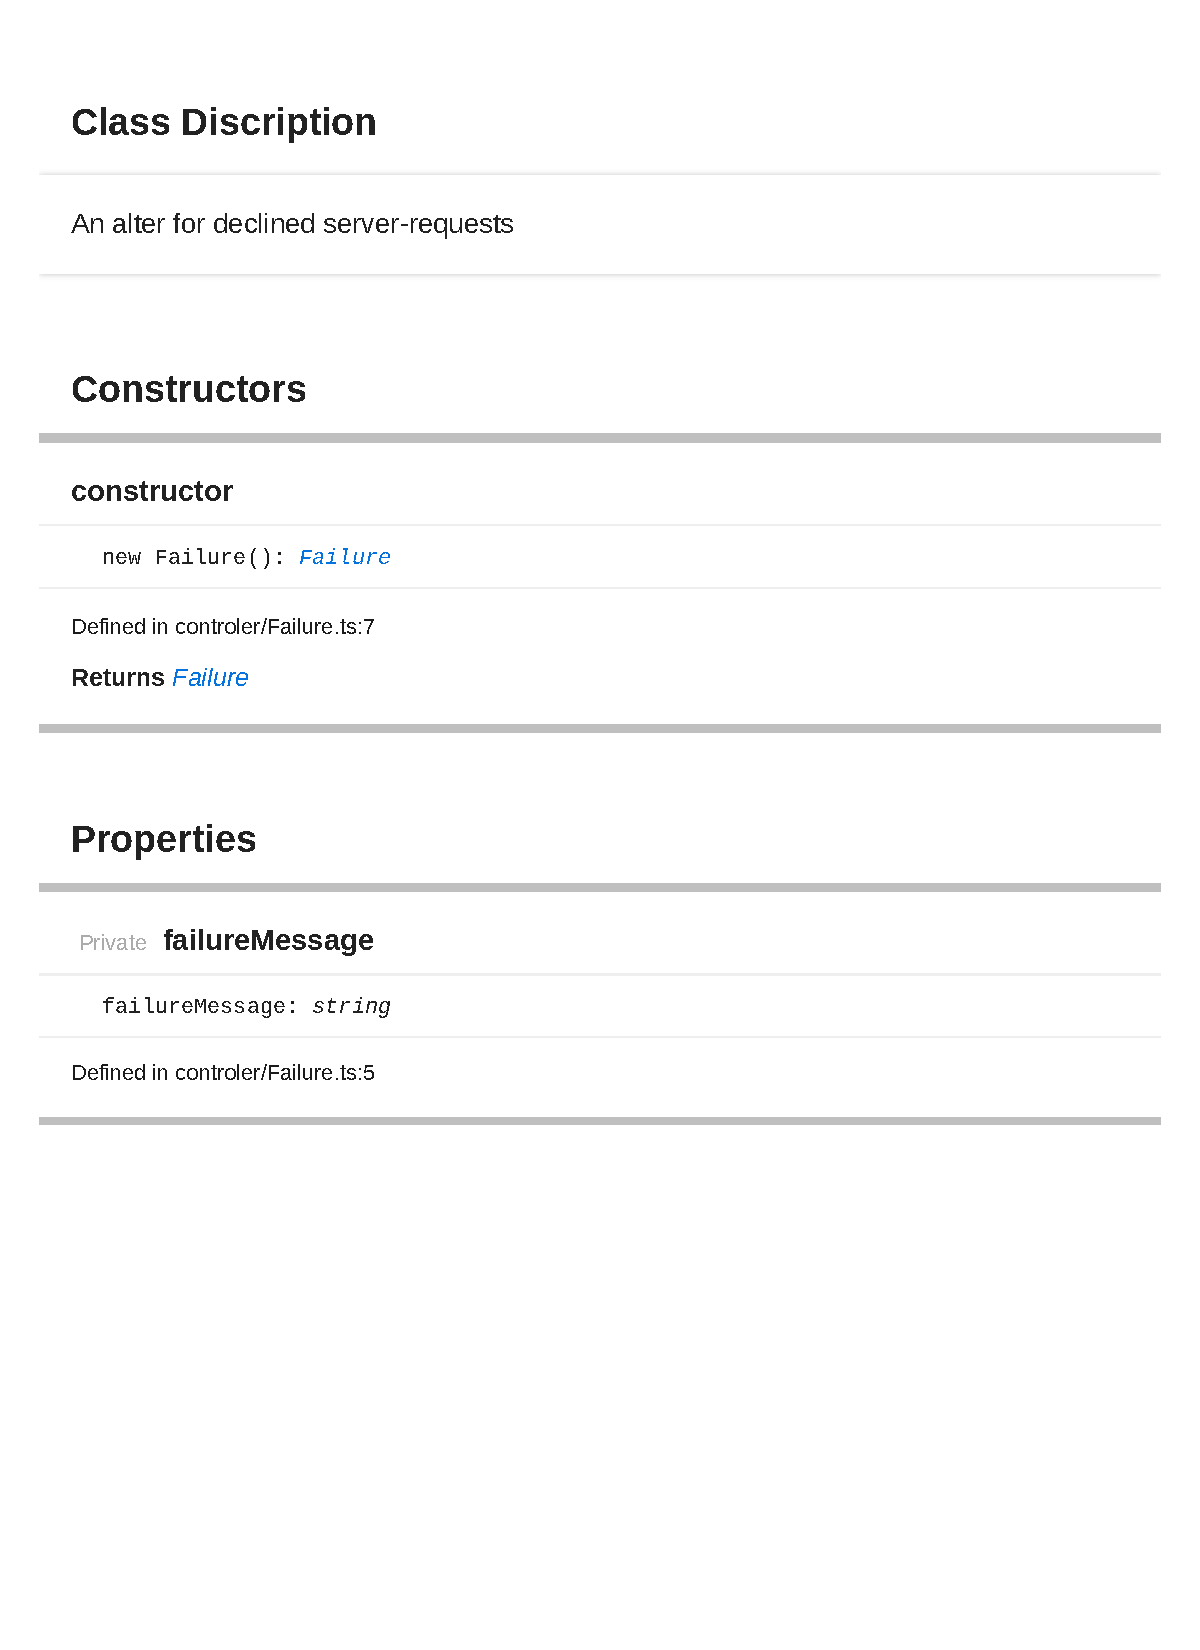
\includepdf[pages=1,  scale=0.8,pagecommand=\class{Failure}]{FrontendDocsAsPDF/Model/Failure.pdf}

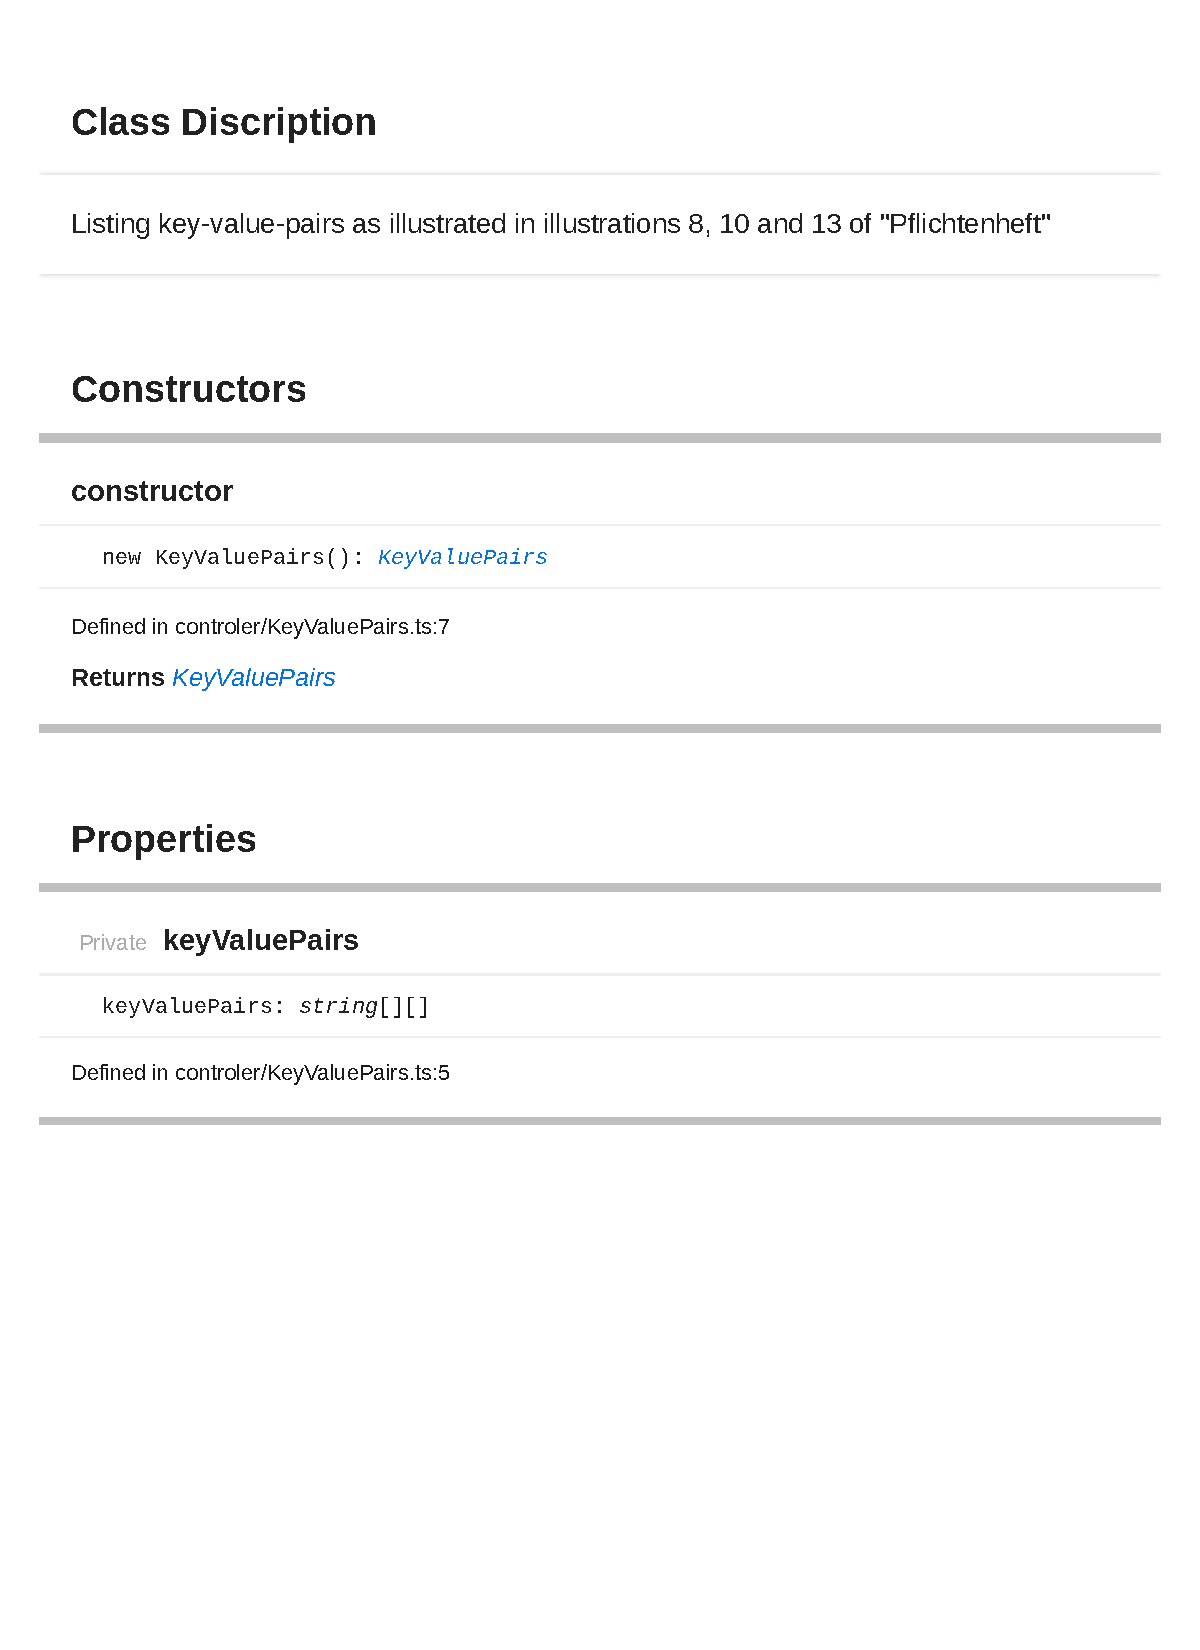
\includepdf[pages=1,  scale=0.8,pagecommand=\class{KeyValuePairs}]{FrontendDocsAsPDF/Model/KeyValuePairs.pdf}

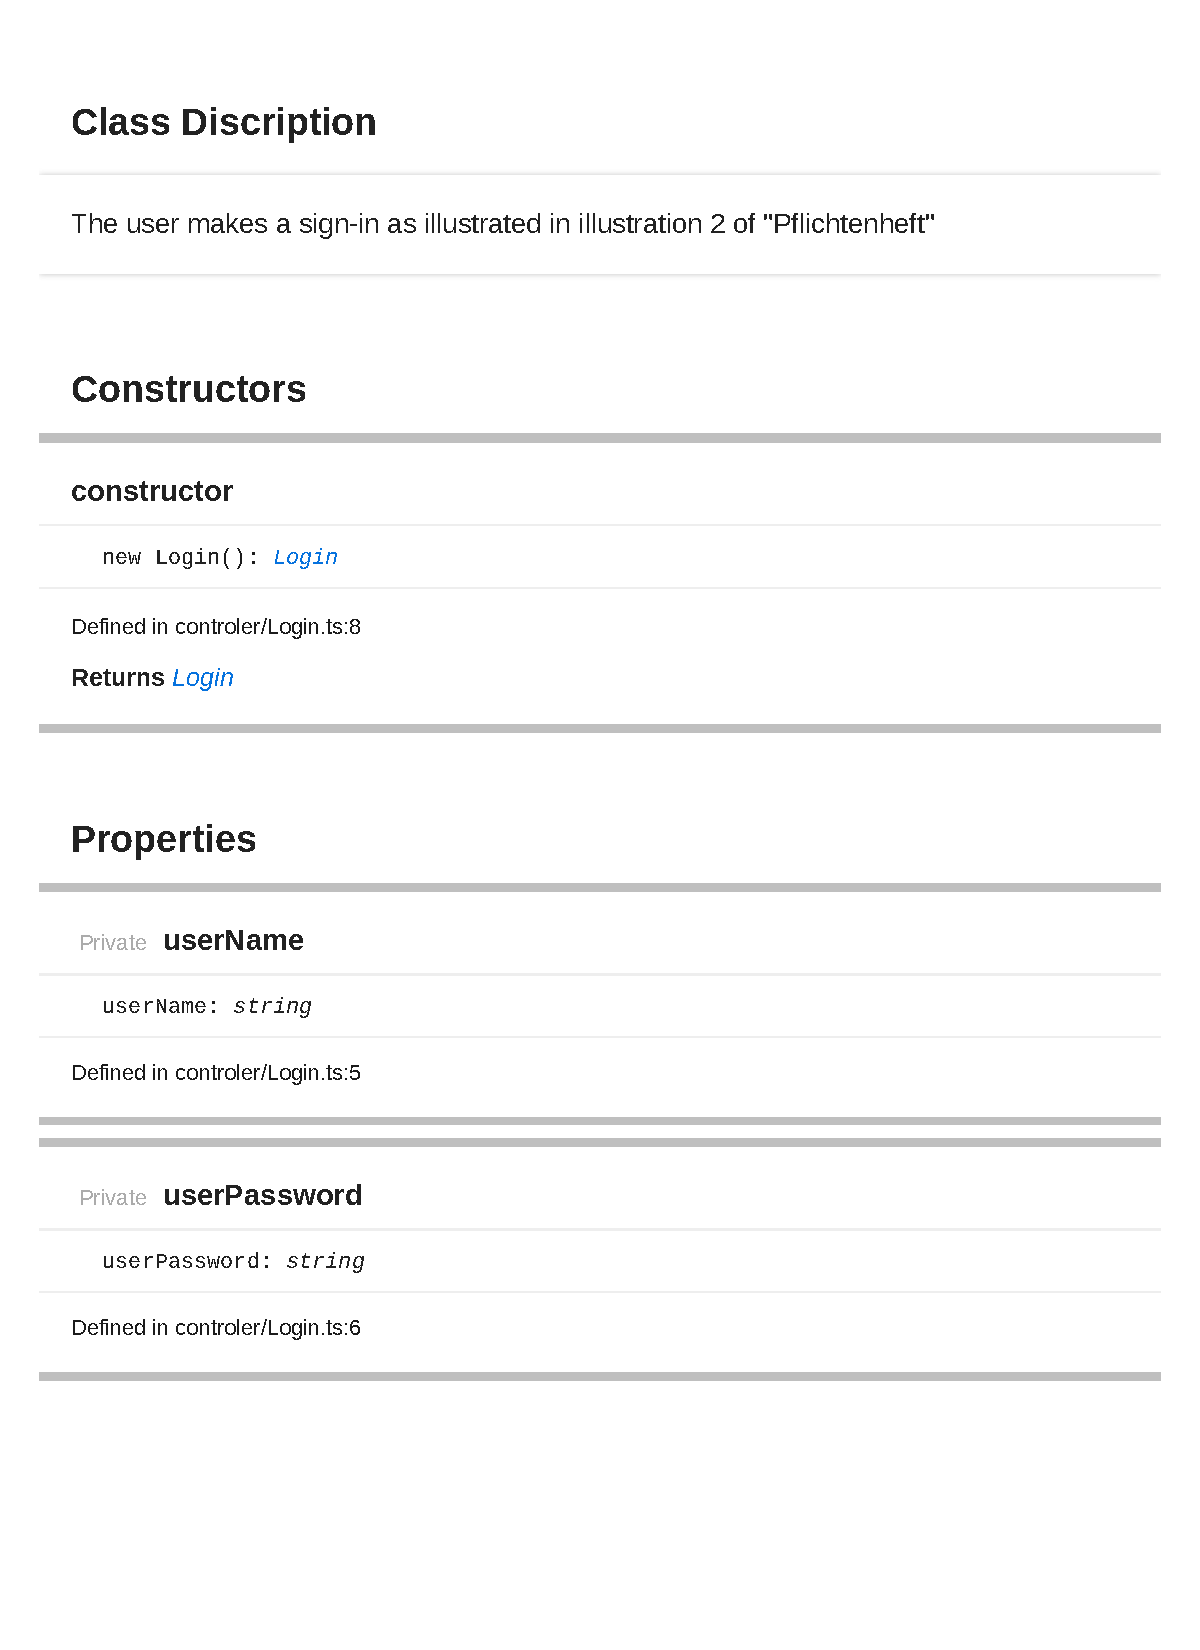
\includepdf[pages=1,  scale=0.8,pagecommand=\class{Login}]{FrontendDocsAsPDF/Model/Login.pdf}

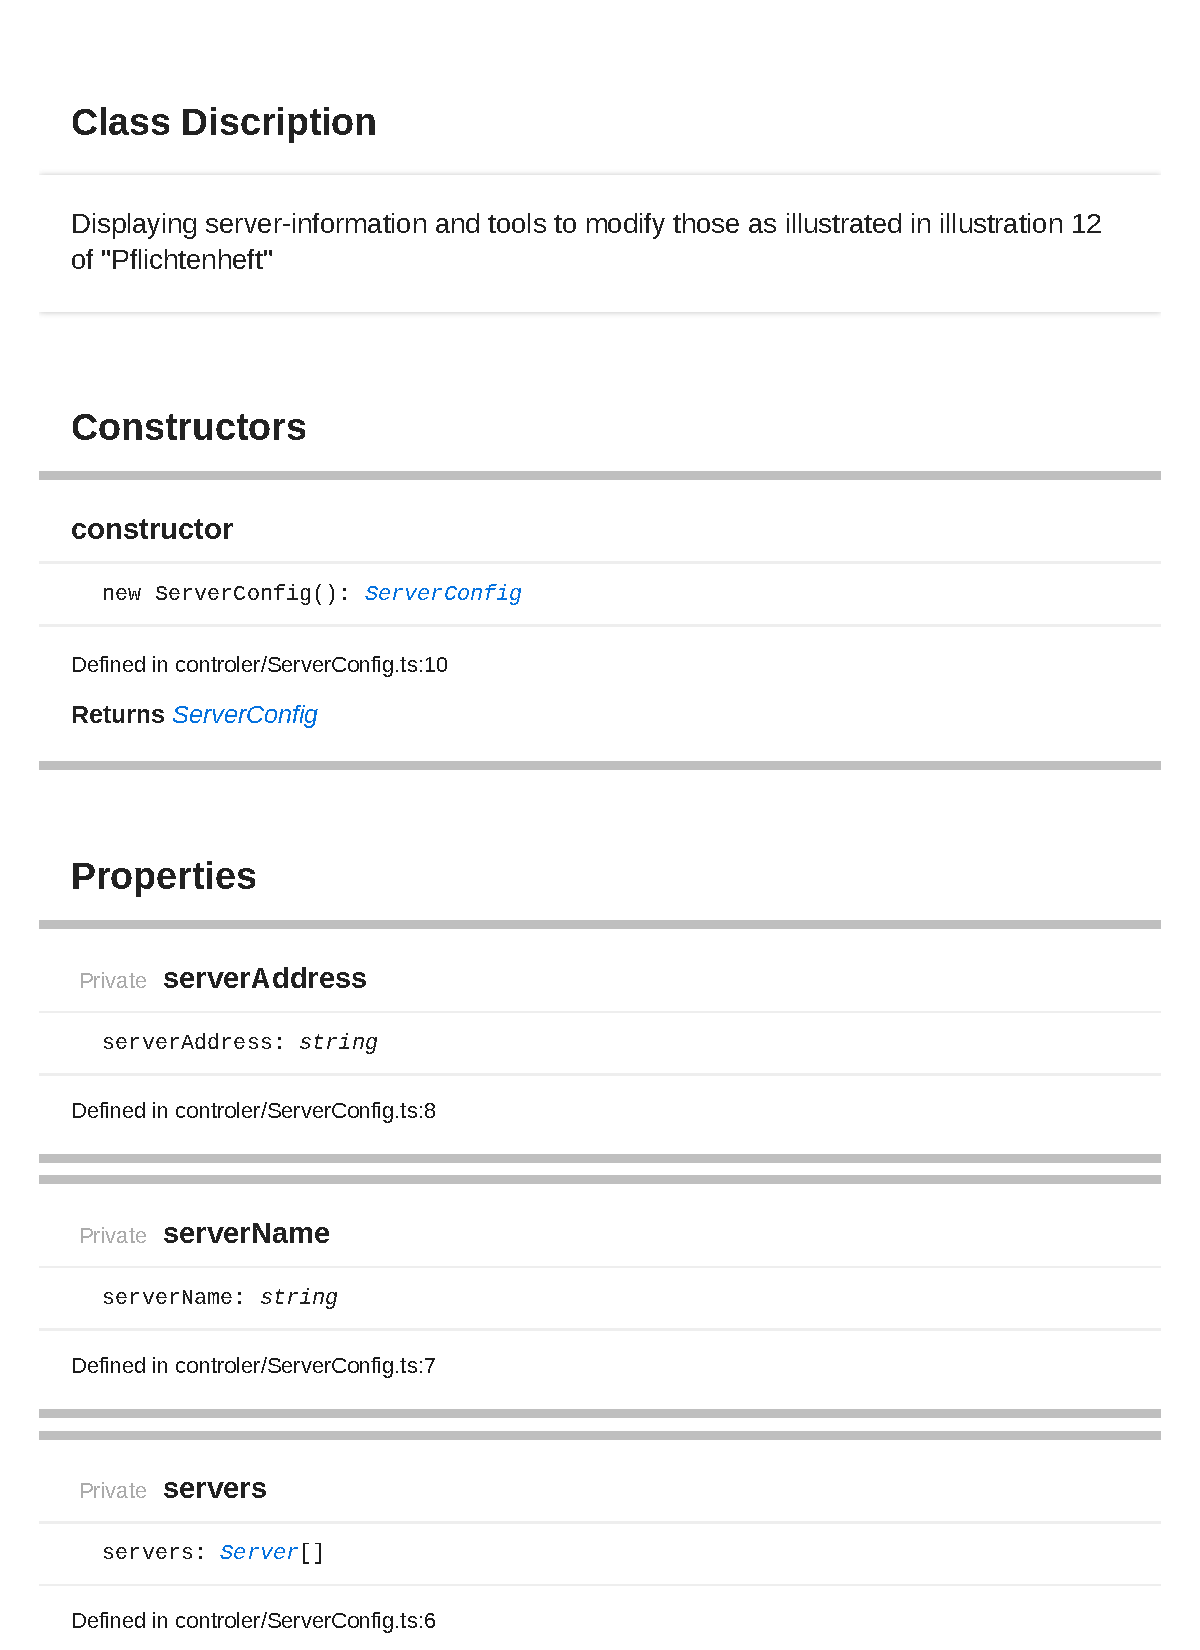
\includepdf[pages=1,  scale=0.8,pagecommand=\class{ServerConfig}]{FrontendDocsAsPDF/Model/ServerConfig.pdf}
\includepdf[pages=2-,  scale=0.8]{FrontendDocsAsPDF/Model/ServerConfig.pdf}

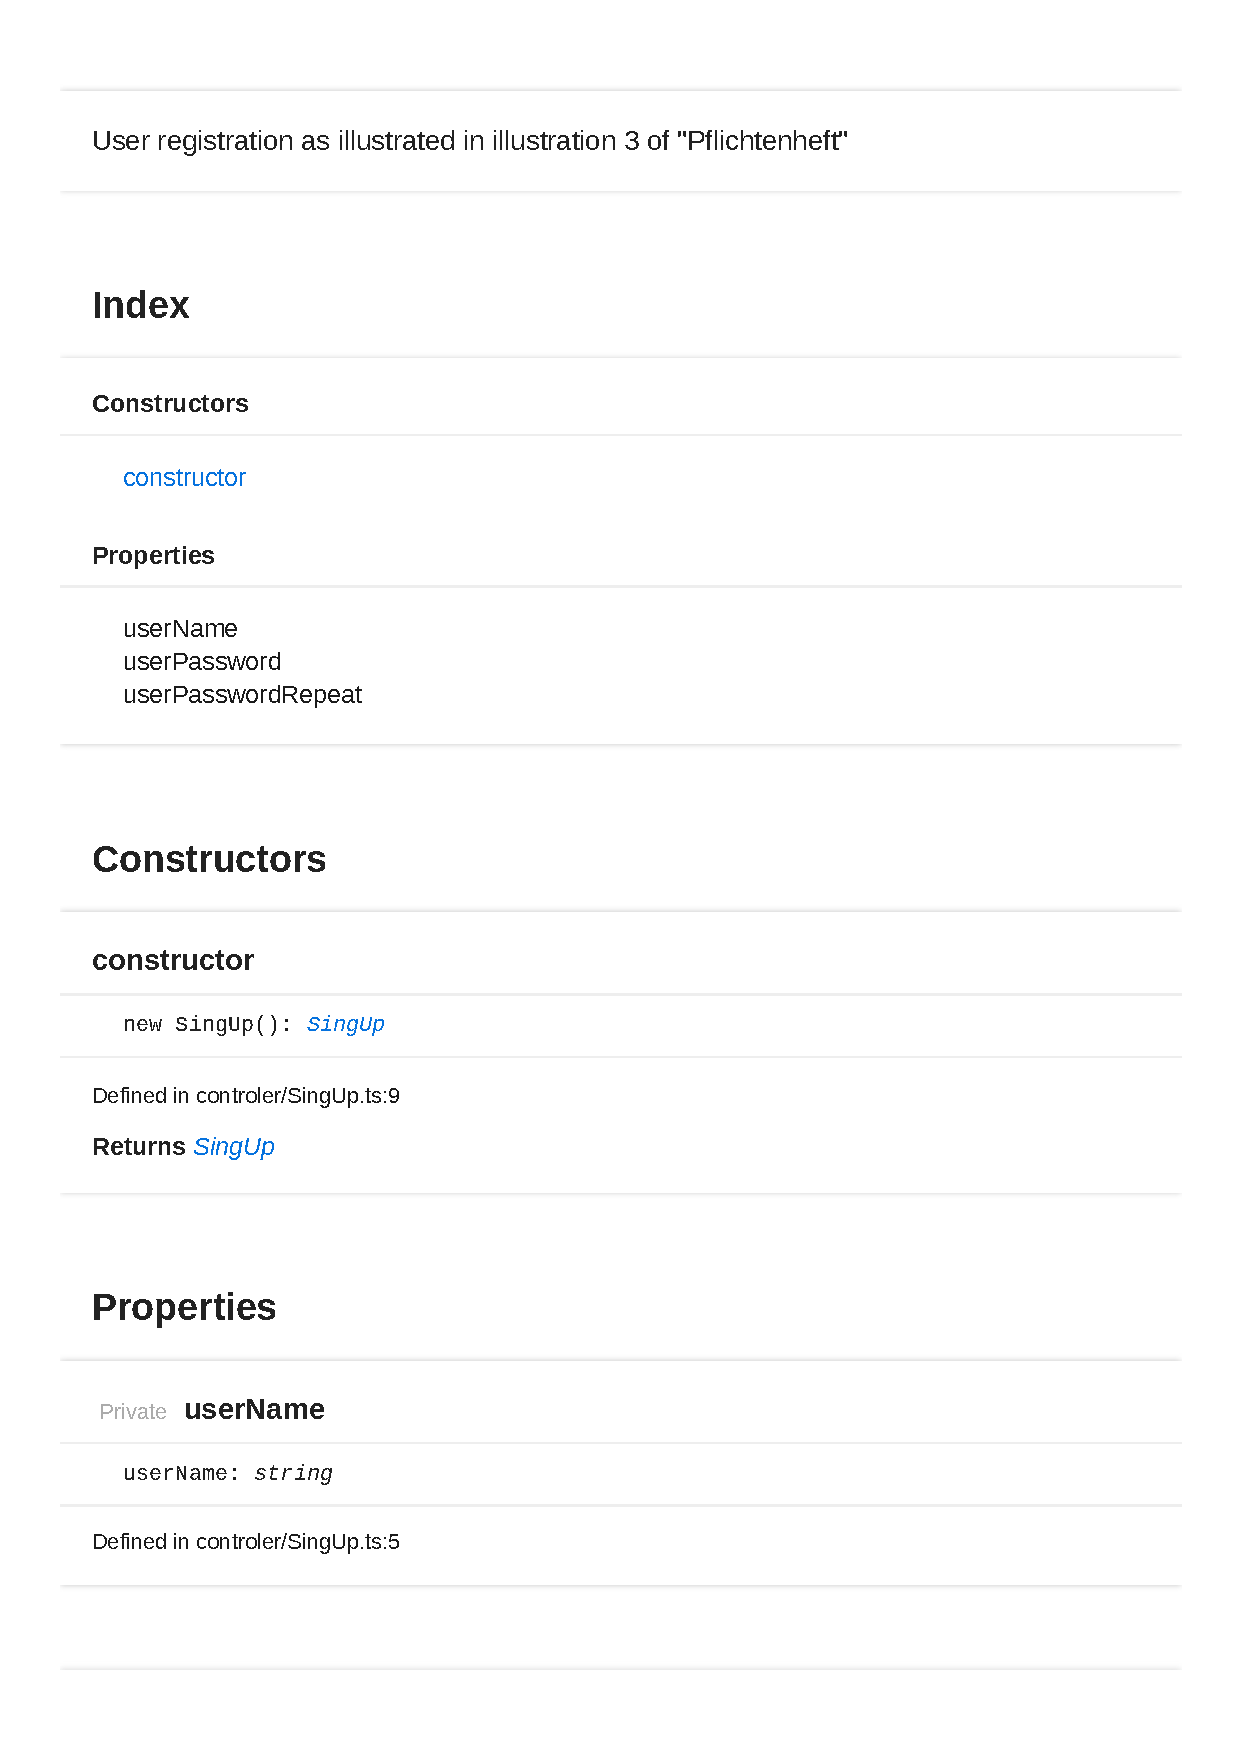
\includepdf[pages=1,  scale=0.8,pagecommand=\class{SignUp}]{FrontendDocsAsPDF/Model/SignUp.pdf}
\includepdf[pages=2-,  scale=0.8]{FrontendDocsAsPDF/Model/SignUp.pdf}

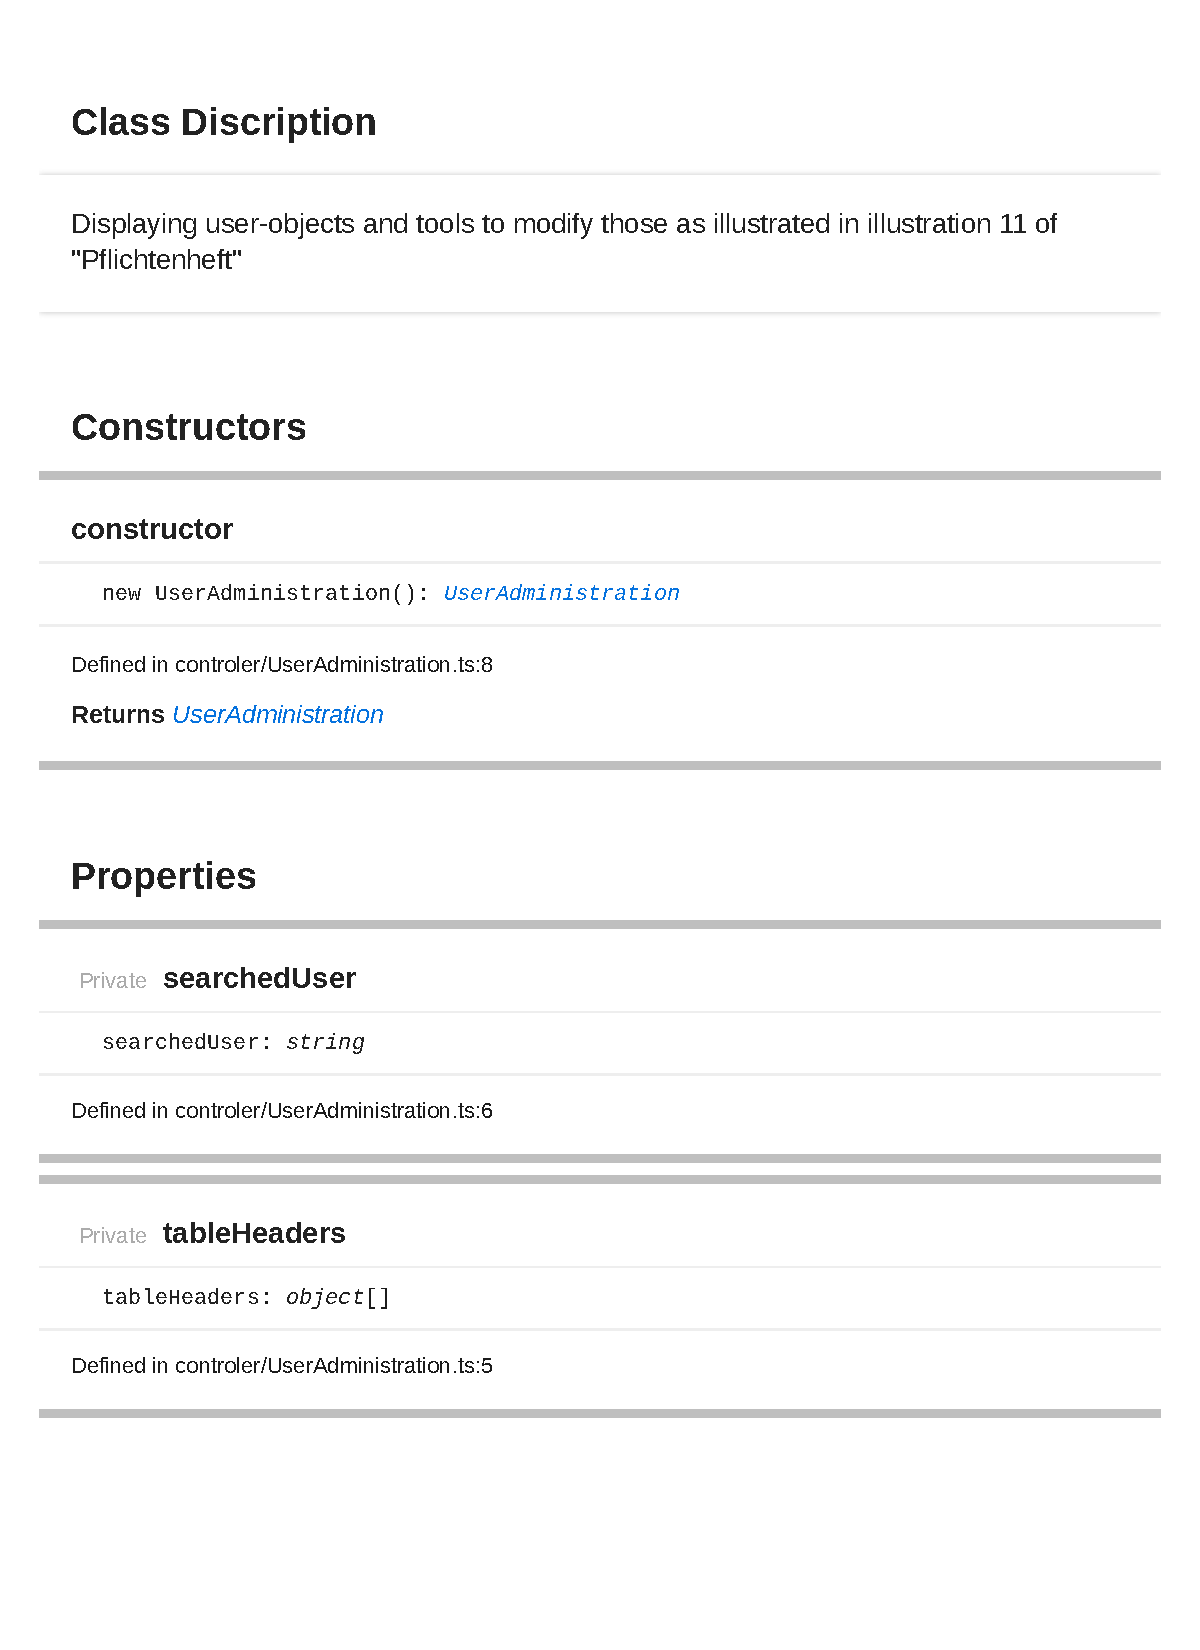
\includepdf[pages=1,  scale=0.8,pagecommand=\class{UserAdministration}]{FrontendDocsAsPDF/Model/UserAdministration.pdf}

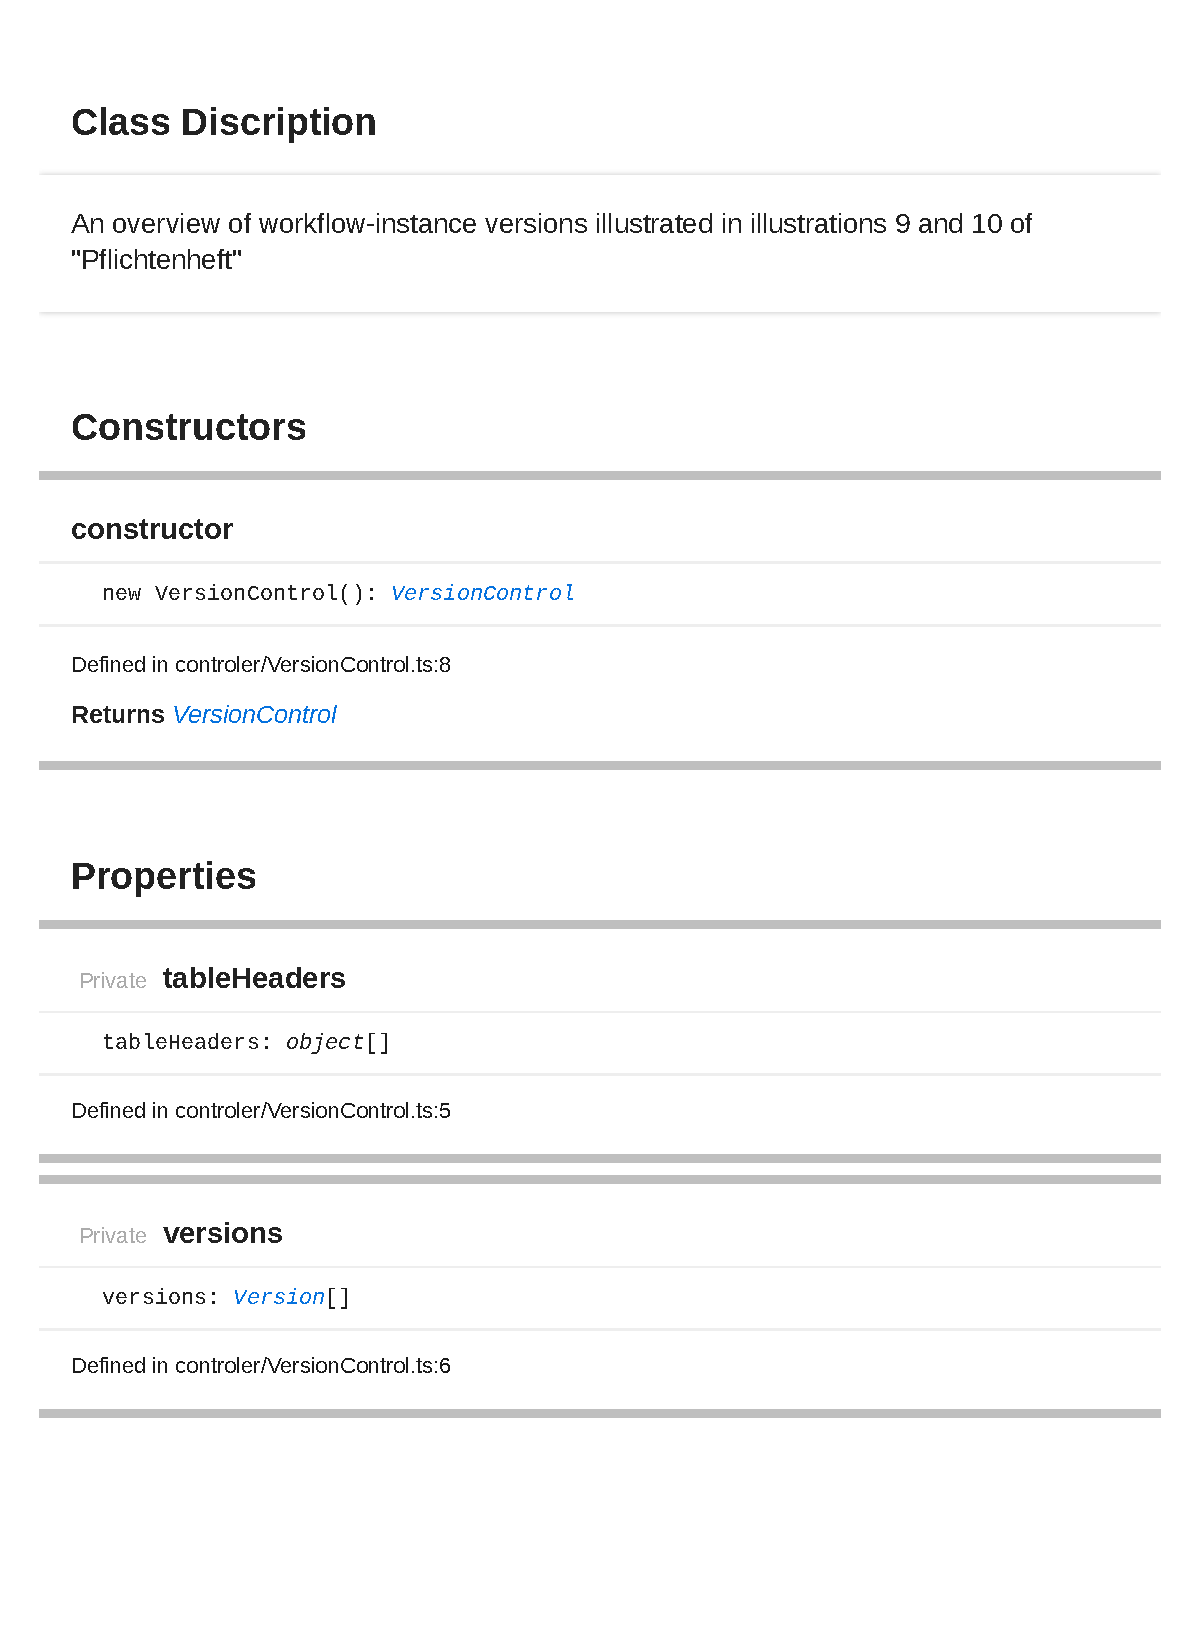
\includepdf[pages=1,  scale=0.8,pagecommand=\class{VersionControl}]{FrontendDocsAsPDF/Model/VersionControl.pdf}

\subsection{Controller}
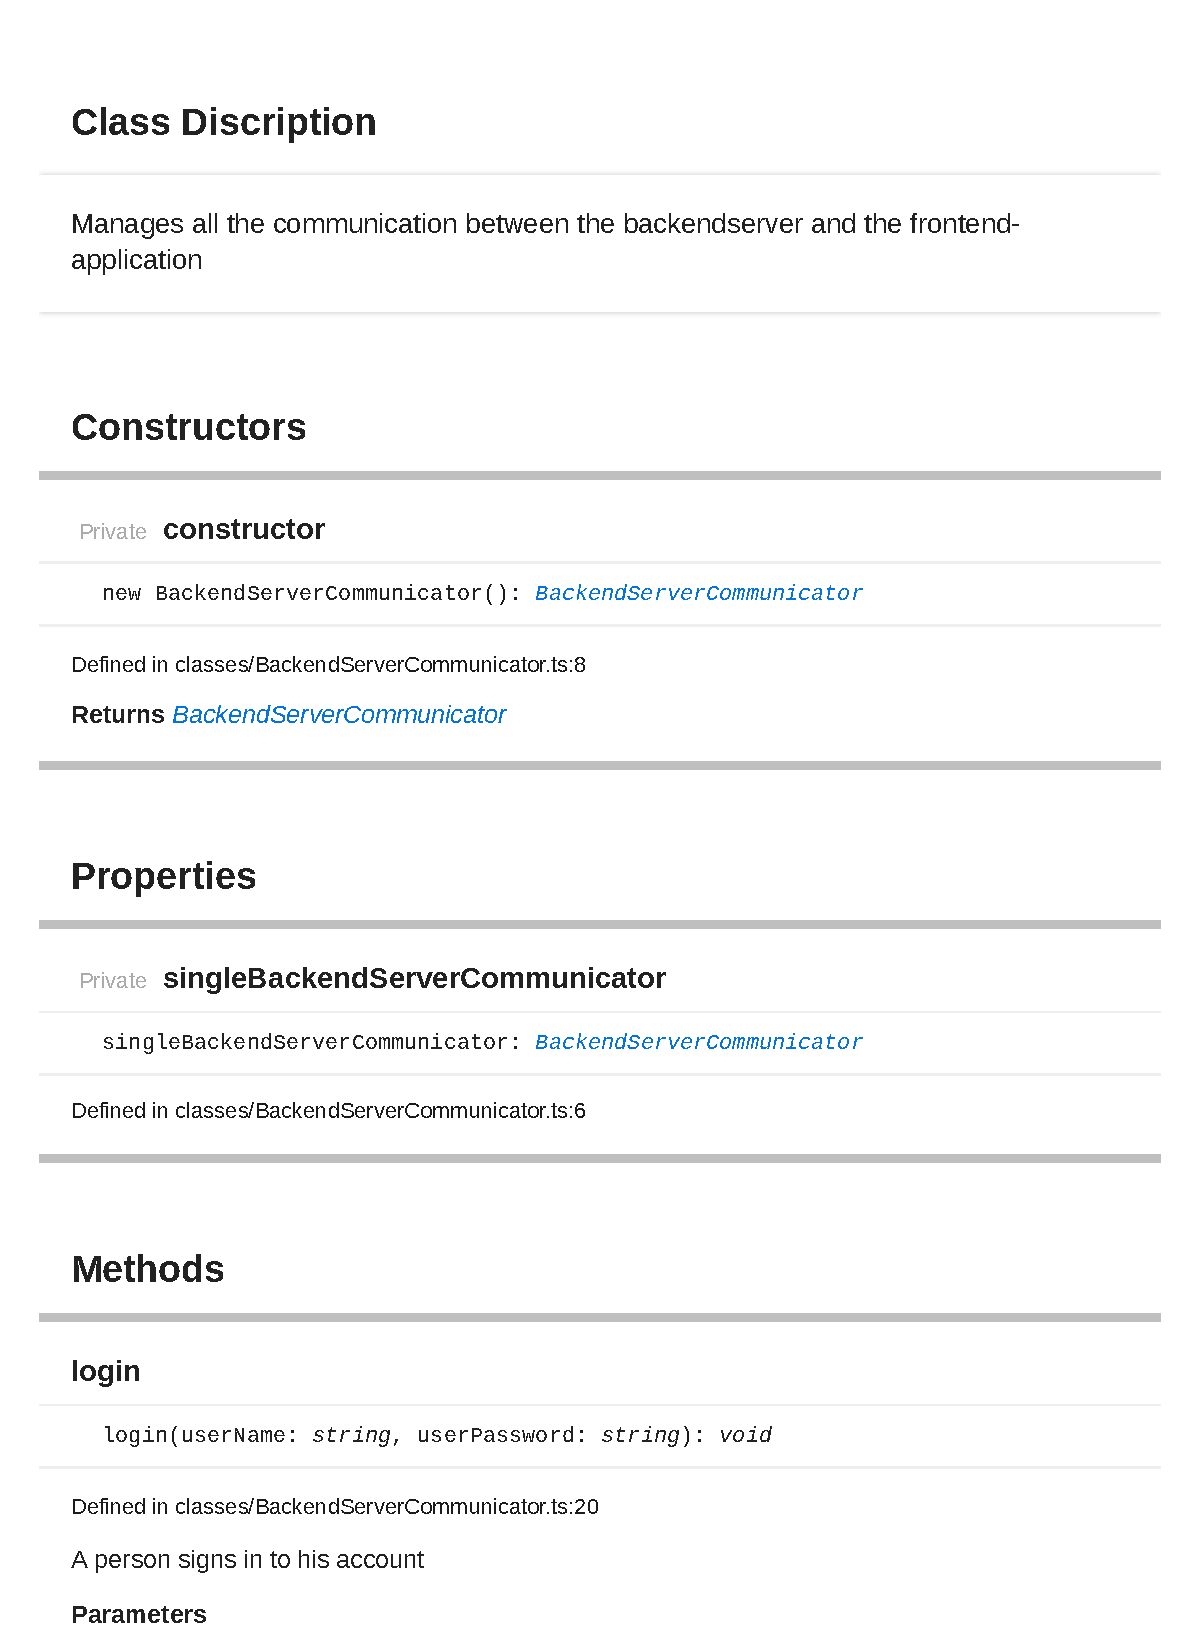
\includepdf[pages=1,  scale=0.8,pagecommand=\class{BackendServerCommunicator}]{FrontendDocsAsPDF/Controller/BackendServerCommunicator.pdf}
\includepdf[pages=2-,  scale=0.8]{FrontendDocsAsPDF/Controller/BackendServerCommunicator.pdf}

\subsubsection{JsonTypeScriptConverter}
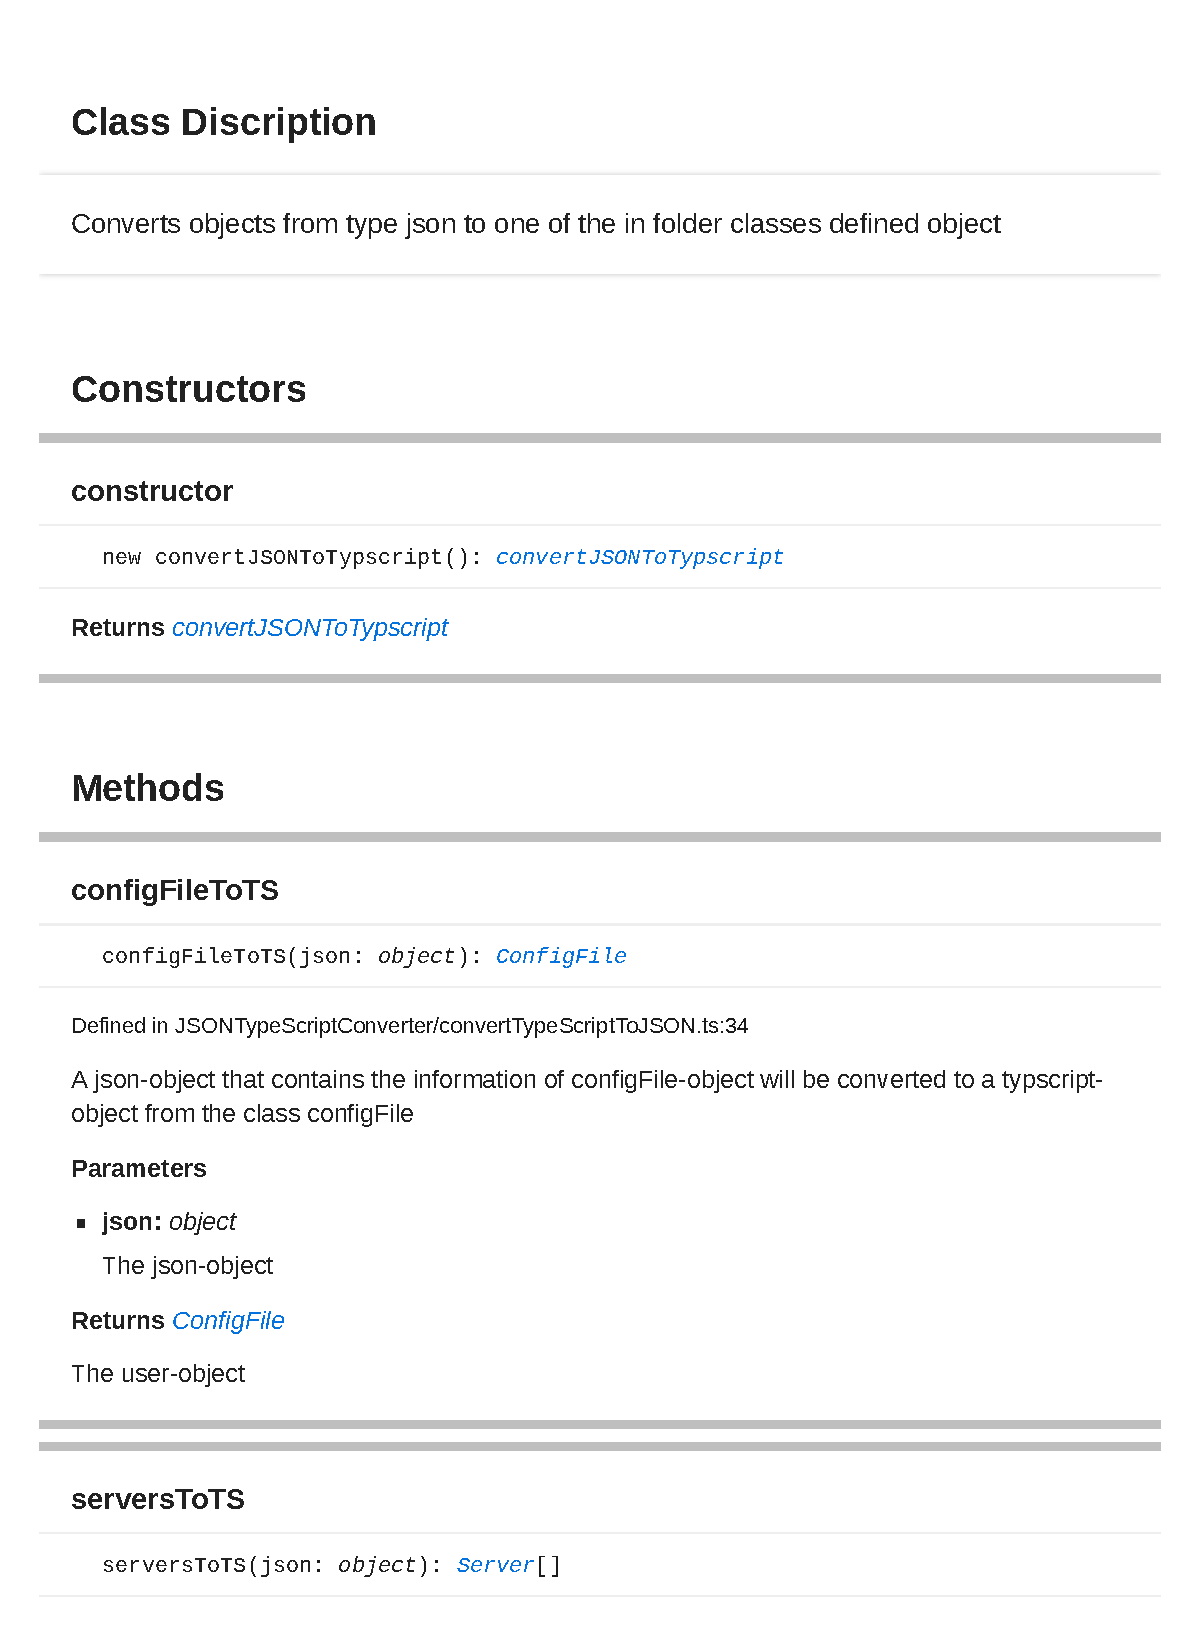
\includepdf[pages=1,  scale=0.8,pagecommand=\class{convertJSONToTypeScript}]{FrontendDocsAsPDF/JSONTypeScriptConverter/convertJSONToTypeScript.pdf}
\includepdf[pages=2-,  scale=0.8]{FrontendDocsAsPDF/JSONTypeScriptConverter/convertJSONToTypeScript.pdf}

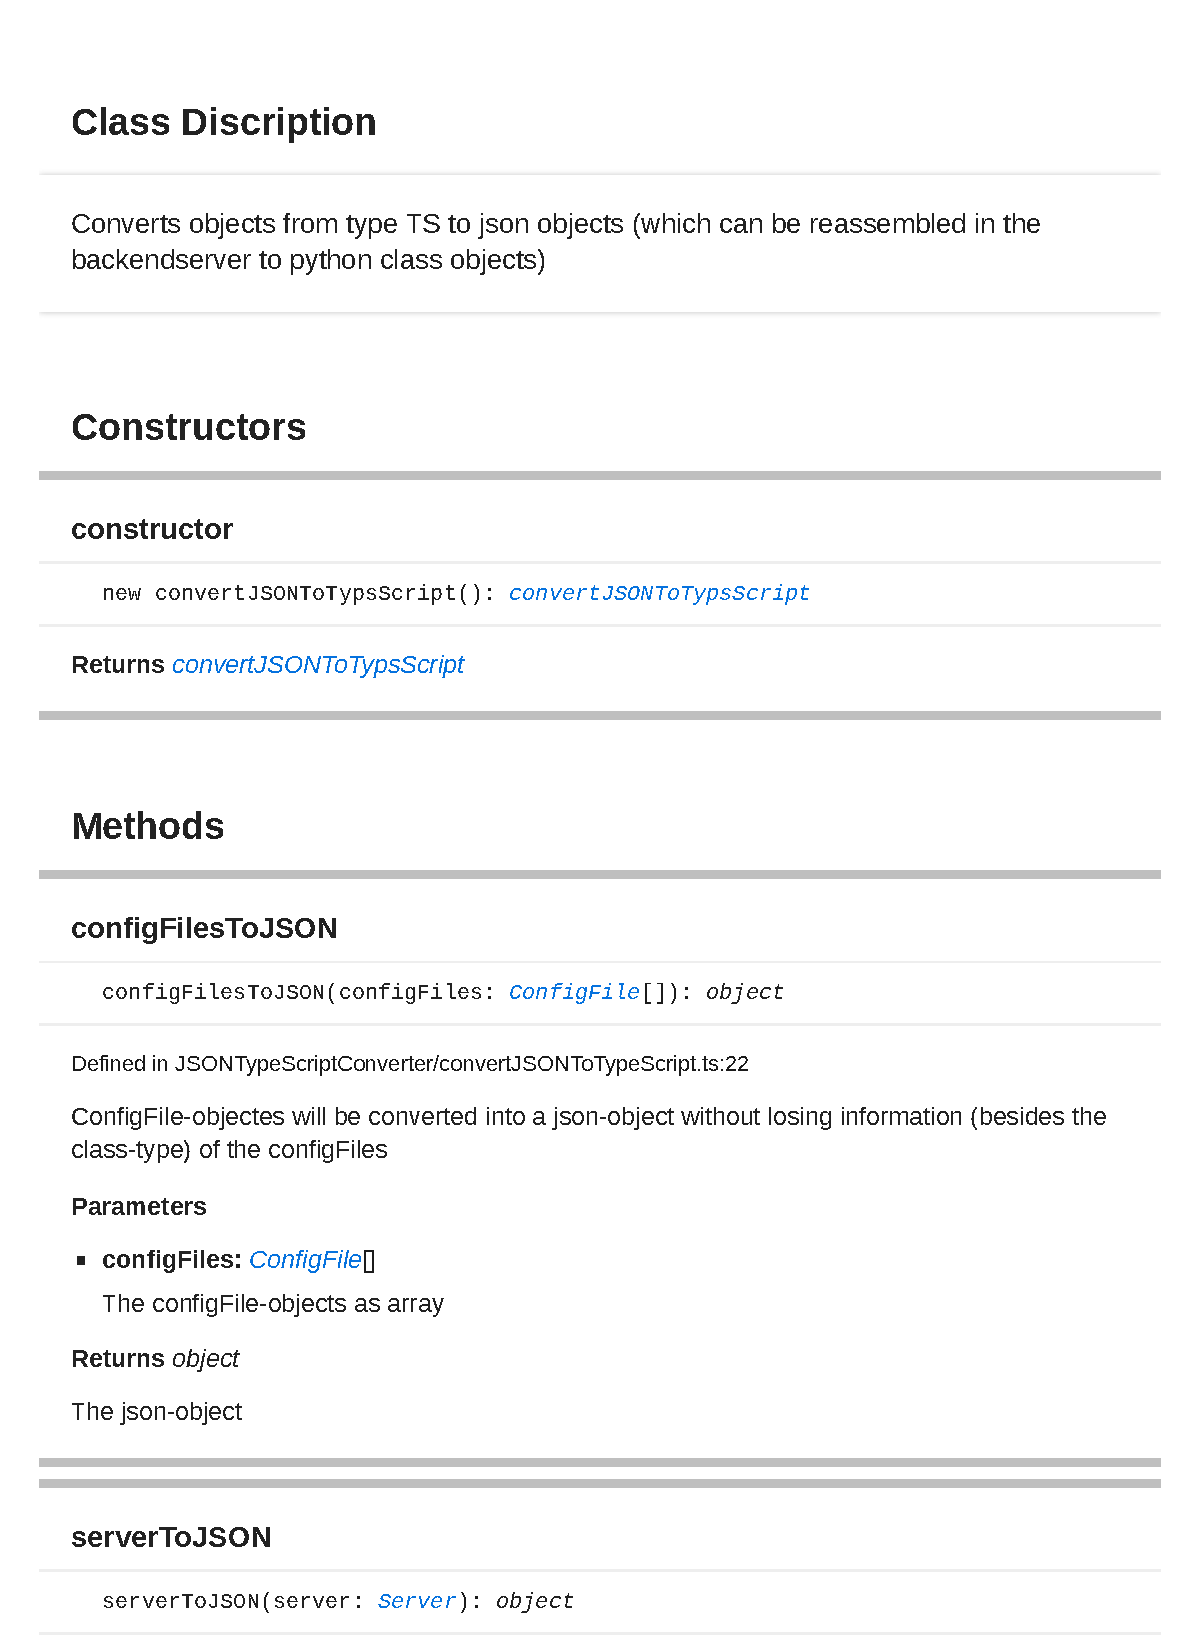
\includepdf[pages=1,  scale=0.8,pagecommand=\class{convertTypsScriptToJSON}]{FrontendDocsAsPDF/JSONTypeScriptConverter/convertTypsScriptToJSON.pdf}
\includepdf[pages=2-,  scale=0.8]{FrontendDocsAsPDF/JSONTypeScriptConverter/convertTypsScriptToJSON.pdf}

\subsubsection{Classes}
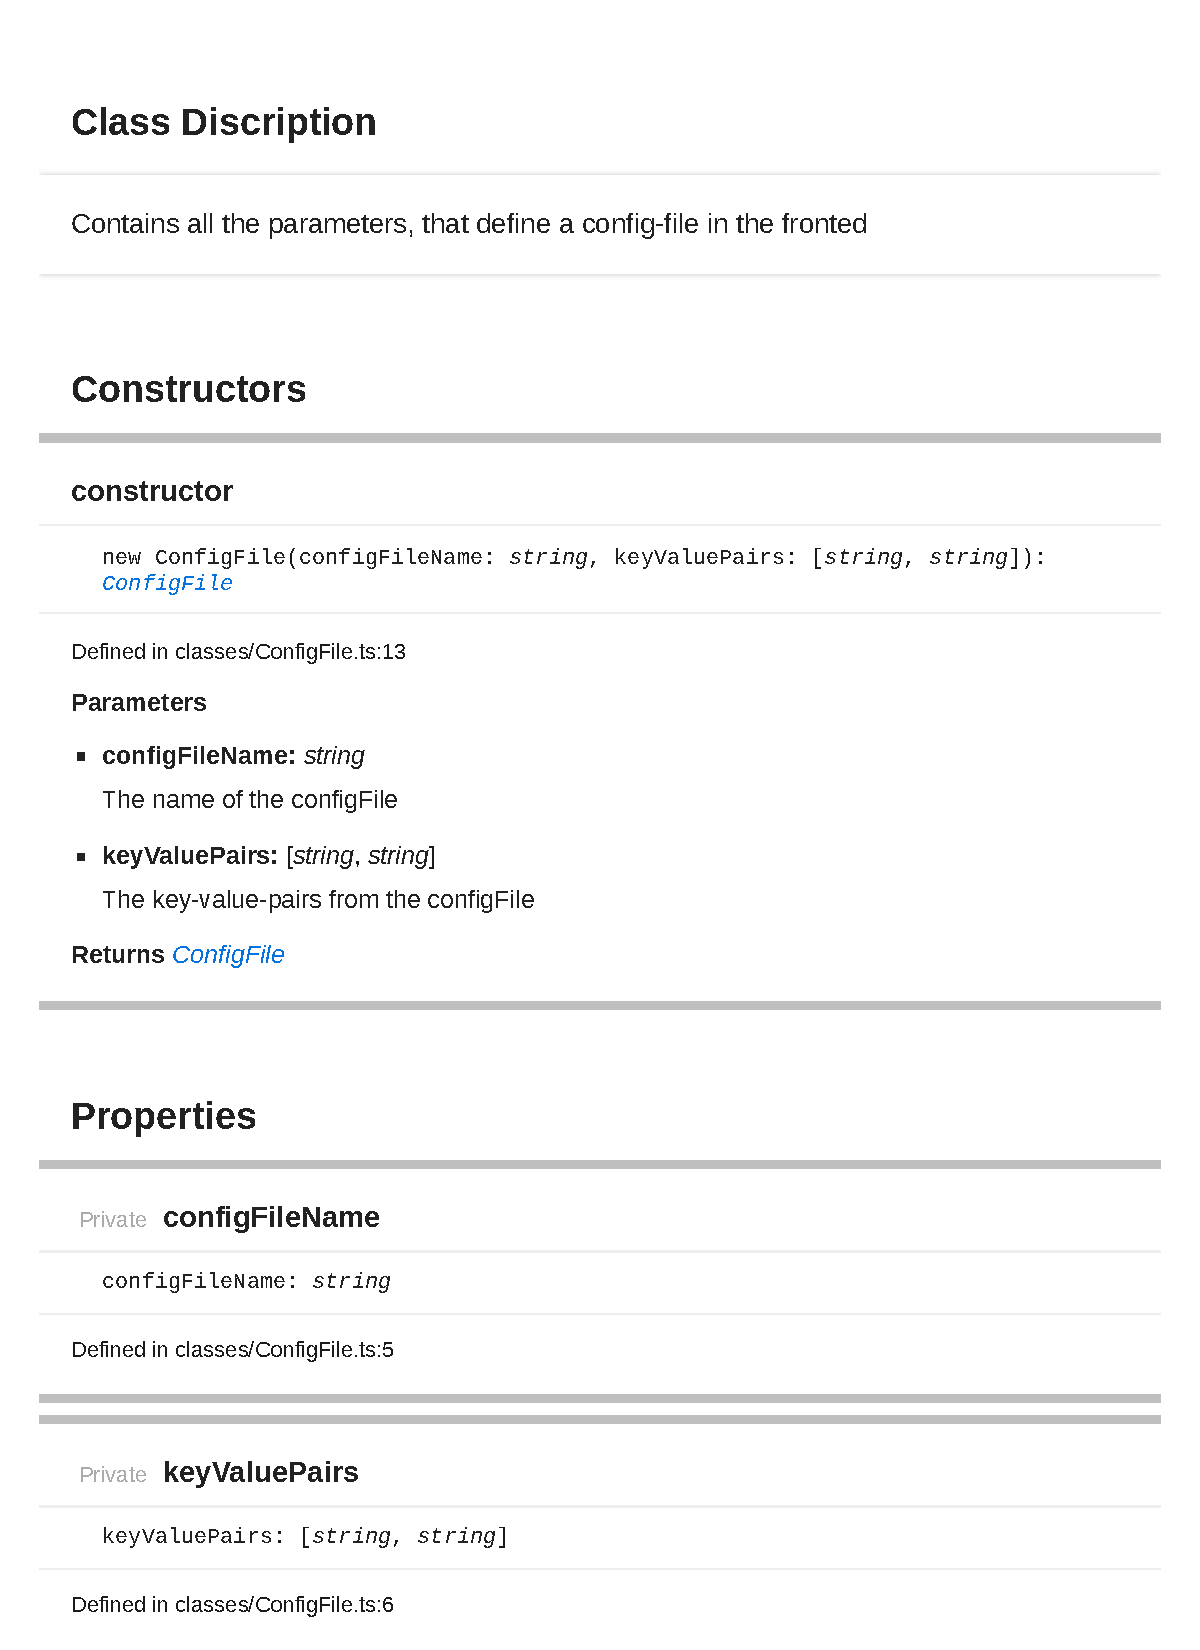
\includepdf[pages=1,  scale=0.8,pagecommand=\class{ConfigFile}]{FrontendDocsAsPDF/Classes/ConfigFile.pdf}

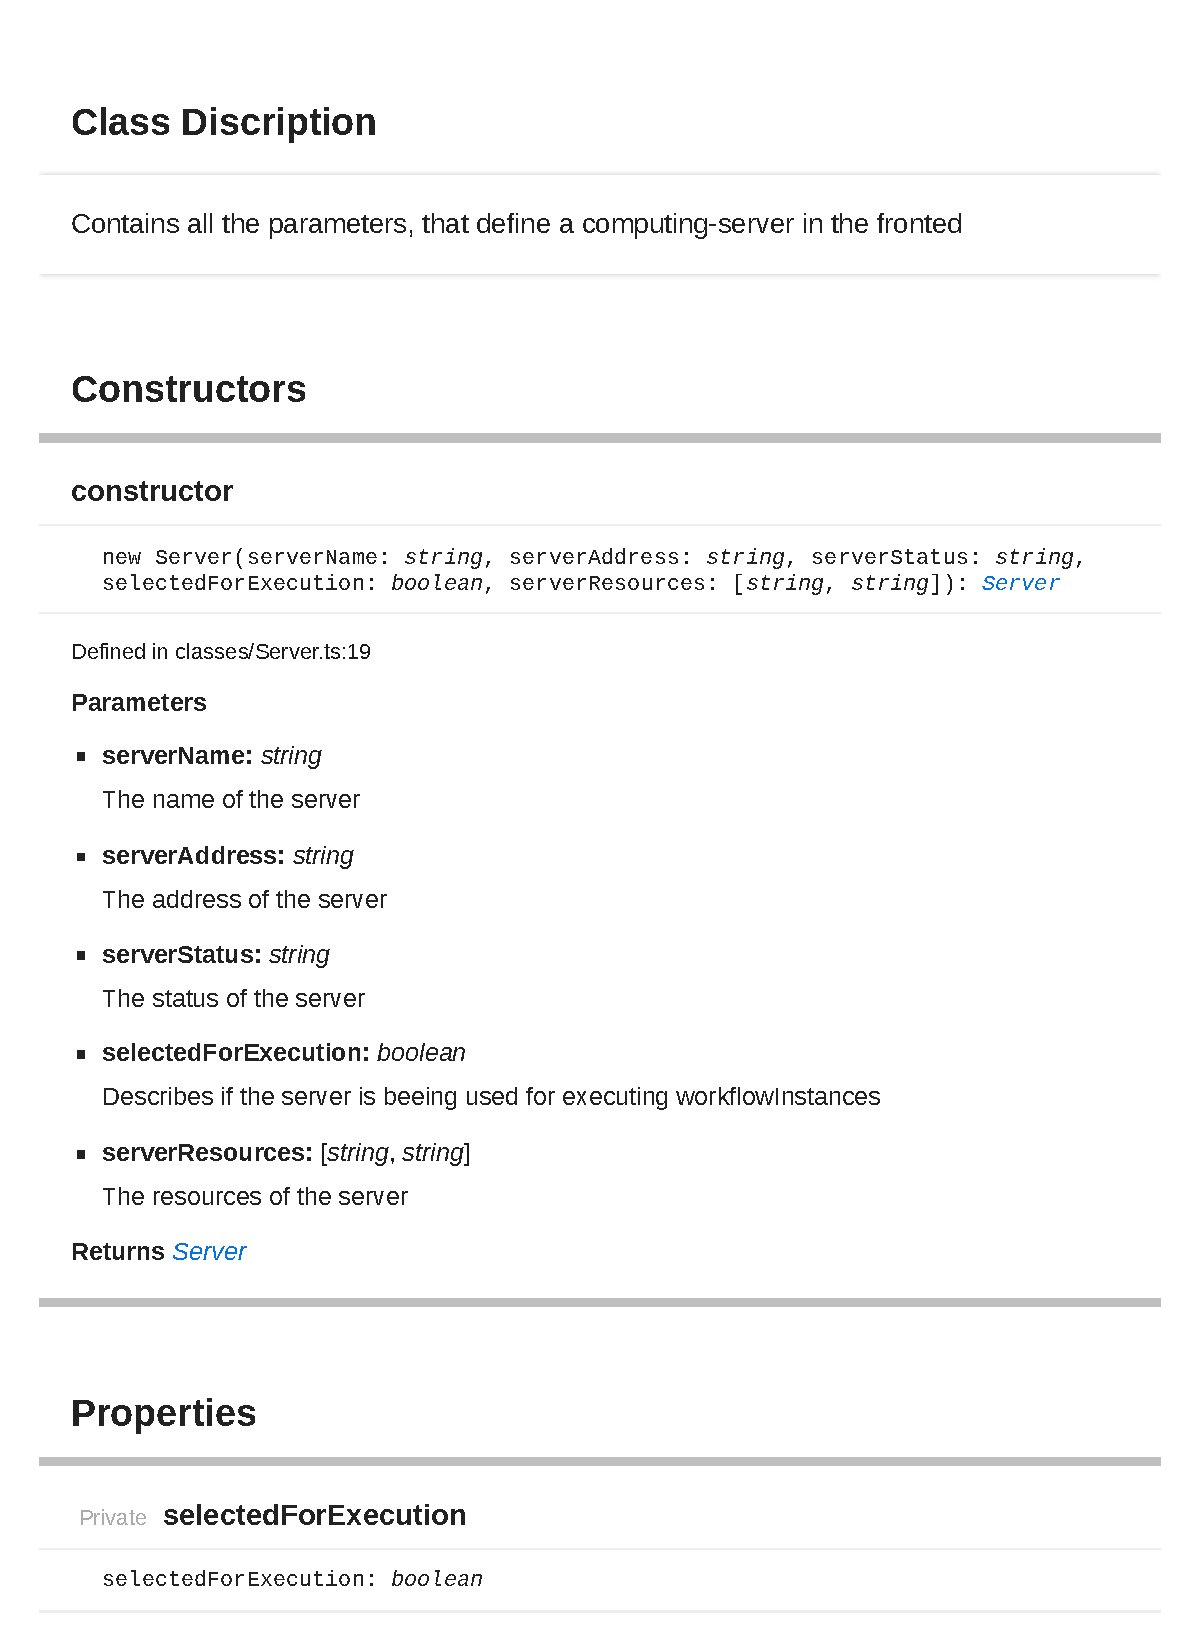
\includepdf[pages=1,  scale=0.8,pagecommand=\class{Server}]{FrontendDocsAsPDF/Classes/Server.pdf}
\includepdf[pages=2-,  scale=0.8]{FrontendDocsAsPDF/Classes/Server.pdf}

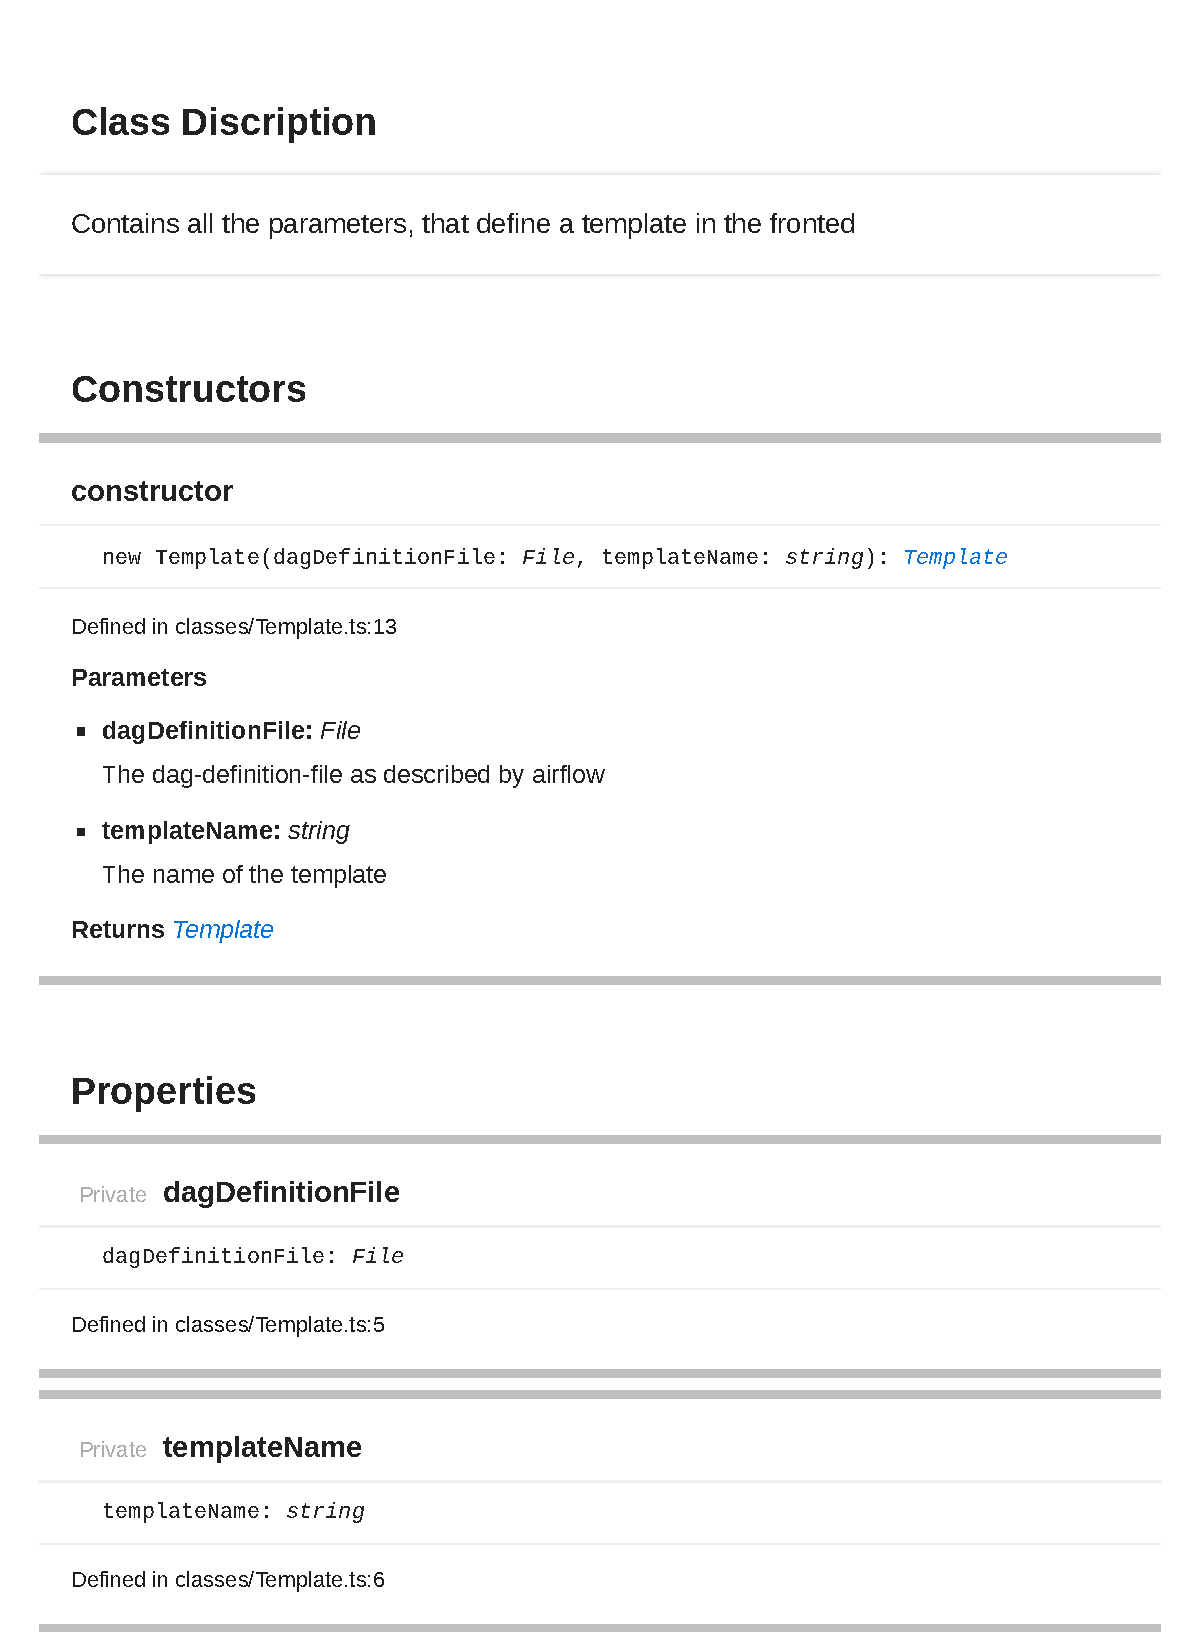
\includepdf[pages=1,  scale=0.8,pagecommand=\class{Template}]{FrontendDocsAsPDF/Classes/Template.pdf}

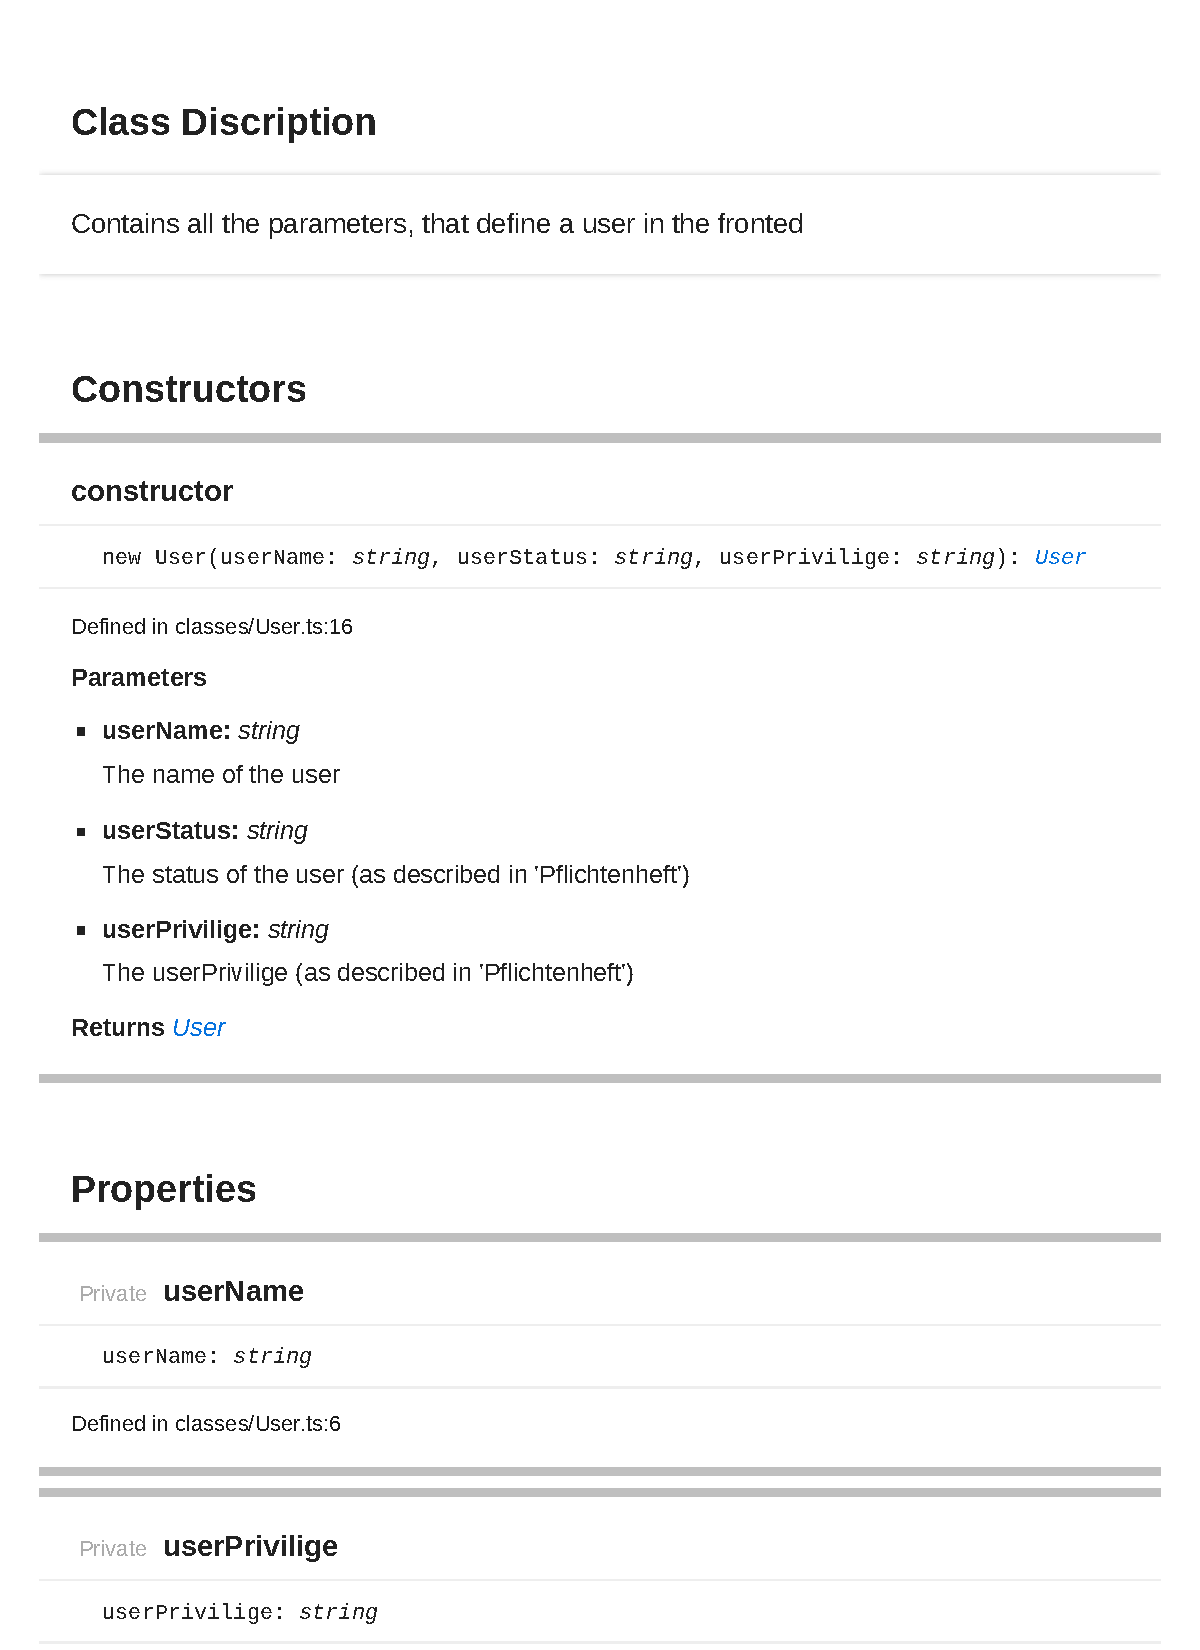
\includepdf[pages=1,  scale=0.8,pagecommand=\class{User}]{FrontendDocsAsPDF/Classes/User.pdf}
\includepdf[pages=2-,  scale=0.8]{FrontendDocsAsPDF/Classes/User.pdf}

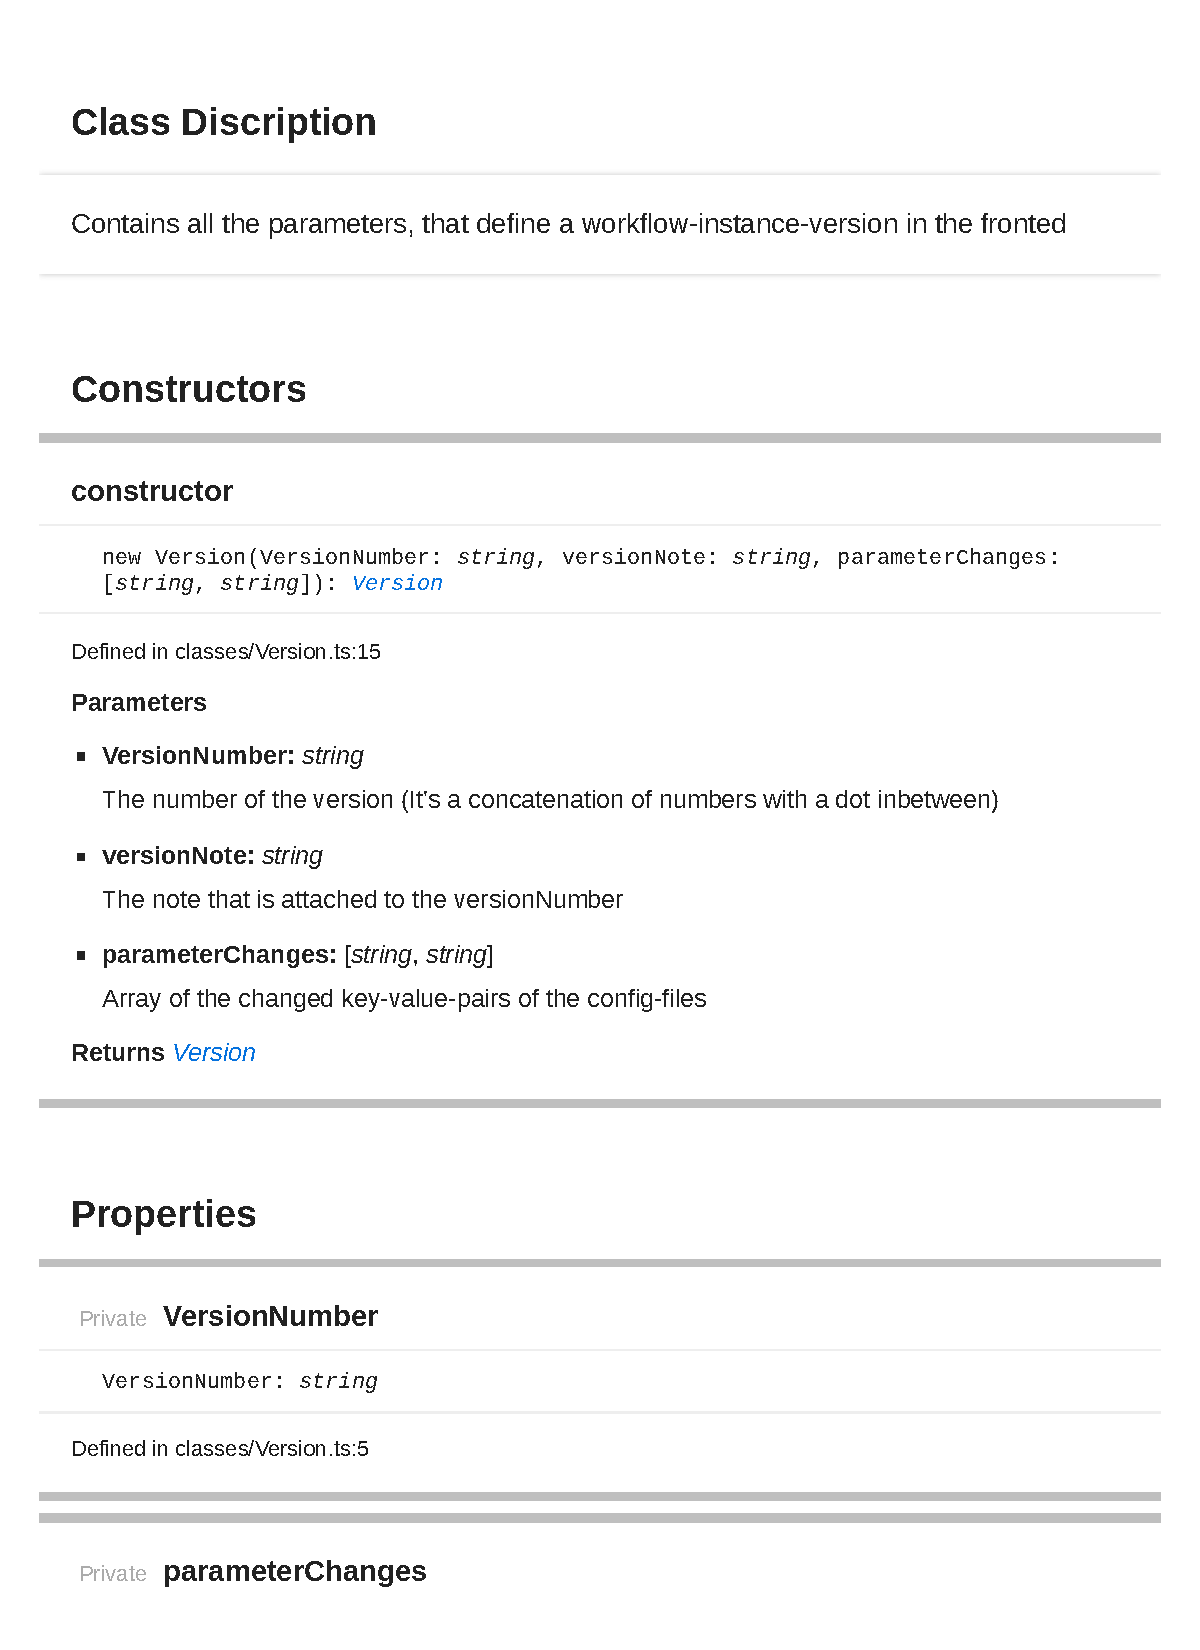
\includepdf[pages=1,  scale=0.8,pagecommand=\class{Version}]{FrontendDocsAsPDF/Classes/Version.pdf}
\includepdf[pages=2-,  scale=0.8]{FrontendDocsAsPDF/Classes/Version.pdf}

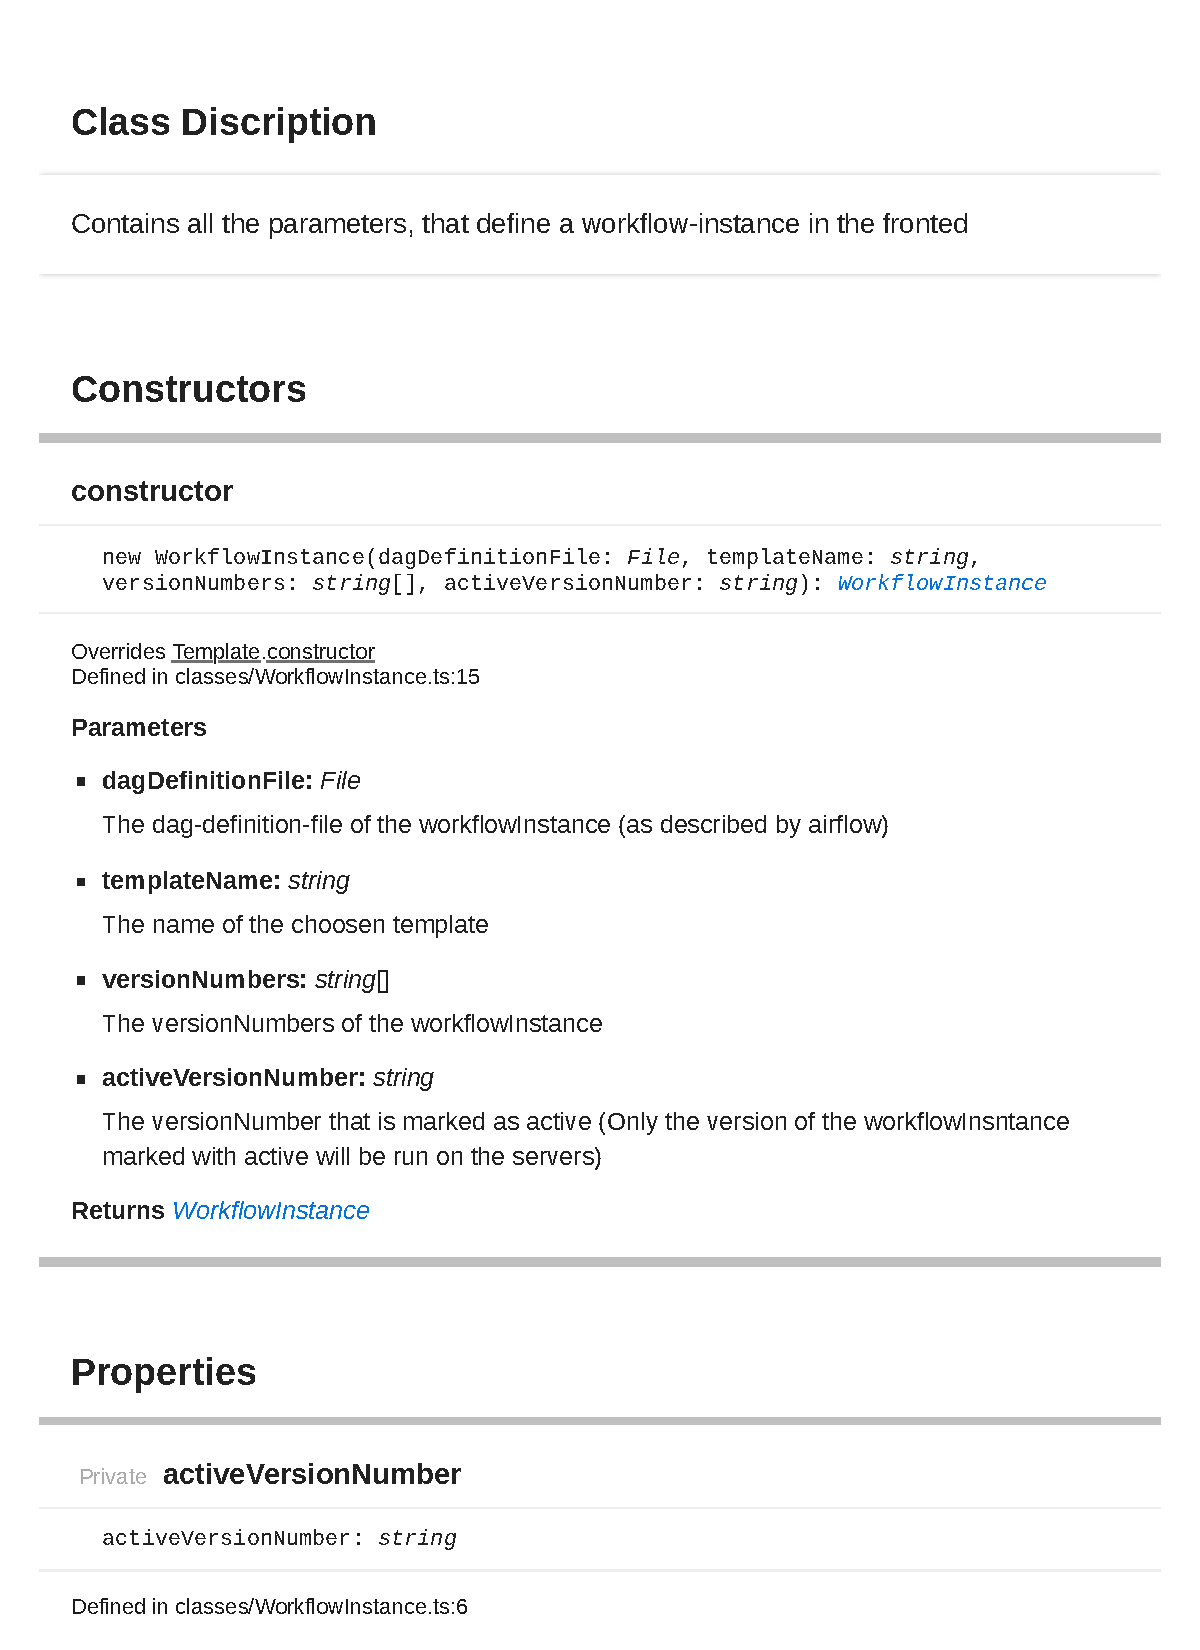
\includepdf[pages=1,  scale=0.8,pagecommand=\class{WorkflowInstance}]{FrontendDocsAsPDF/Classes/WorkflowInstance.pdf}
\includepdf[pages=2-,  scale=0.8]{FrontendDocsAsPDF/Classes/WorkflowInstance.pdf}

\subsection{Server Application}
\subsubsection{API Package}
\paragraph{Package: api} This package is the interface between the client's application and the server application. 
All requests are sent to this API(package) in JSON format.

\paragraph{Class: FrontendAPI}

This class is the main interface of the whole application.The decision to design FrontendAPI as
 \textbf{Singleton} pattern means that the API should be a globally accessible instance that runs on the server
on a certain port. The way this happens happens is an  implementation detail with which the framework
\textbf{Flask} helps, but the base idea must be respected in the software design decision. The client application
can get the api status code to obtain information regarding the execution of api calls (e.g. status code
changes when an exception has been thrown)

\subparagraph{static get\texttt{\_}FrontendAPI(): FrontendAPI} returns the FrontendAPI in singleton design fashion, meaning 
there is only one instance of FrontendAPI in circulation at all times.

\subparagraph{get\texttt{\_}status\texttt{\_}code(): int} return status code  

\subparagraph{set\texttt{\_}status\texttt{\_}code(status\texttt{\_}code: int)}
sets the status code, only performed by the \textbf{ExceptionHandler}
\begin{itemize}
        \item \textbf{status\texttt{\_}code}
        the status code showing the state of the latest API call
\end{itemize}

\subparagraph{get\texttt{\_}server\texttt{\_}details(): String}
gets all server details (container limit, cpu resources, gpu resources, servername, ip address, executing server (yes/no)) 
and returns them in a json format (json.dumps is interpreted as String in native python)

\subparagraph{set\texttt{\_}server\texttt{\_}details(json\texttt{\_}details: String)}
sets all server details (container limit, cpu resources, gpu resources, servername, ip address, executing server (yes/no)) in
 a json format (json objects are interpreted as String in native python). Only one bulk update as a whole
due to long delay with server communication from client's perspective
\begin{itemize}
        \item \textbf{server\texttt{\_}details}
        all server details in json format
\end{itemize}

\subparagraph{get\texttt{\_}all\texttt{\_}users\texttt{\_}and\texttt{\_}details(): String}
gets all users and their details (user names, privileges, statuses) in a json format
(json objects are interpreted as String in native python). Only one bulk update as a whole
due to long delay with server communication from client's perspective


\subparagraph{set\texttt{\_}all\texttt{\_}users\texttt{\_}and\texttt{\_}details(json\texttt{\_}details: String)}
sets all user details (user name, privilege, statuse) for a specific user in a json format
(json objects are interpreted as String in native python). Only one bulk update as a whole
due to long delay with server communication from client's perspective. If user does not already exist, one will be created.

\subparagraph{delete\texttt{\_}user(json\texttt{\_}details: String)}
deletes a user by username
\begin{itemize}
        \item \textbf{json\texttt{\_}details}
        json object which only contains the username key and value
\end{itemize}


%ab hier wf
\subparagraph{get\texttt{\_}wf\texttt{\_}instance\texttt{\_}version\texttt{\_}number
(json\texttt{\_}details: String): String}
returns a json object containing workflow instance's version number key and value
\begin{itemize}
        \item \textbf{json\texttt{\_}details}
        json object which only contains the workflow instance name and version number key and value
\end{itemize}

\subparagraph{replace\texttt{\_}wf\texttt{\_}instance\texttt{\_}version\texttt{\_}number
(json\texttt{\_}details: String)}
replaces the (active) workflow instance's version number 
\begin{itemize}
        \item \textbf{json\texttt{\_}details}
        json object which only contains the workflow instance name key and value and version number key and value
\end{itemize}


\subparagraph{set\texttt{\_}config\texttt{\_}file(json\texttt{\_}details)}
changes multiple config files based on input/ key value pair changes in client's applications during workflow instance 
configuration
\begin{itemize}
        \item \textbf{json\texttt{\_}details}
        json object which contains the changed config files and respectively their changed values, contains workflow
        instance key and value
\end{itemize}

\subparagraph{get\texttt{\_}config\texttt{\_}from\texttt{\_}wf\texttt{\_}instance(json\texttt{\_}details): String}
gets all config file names related to specific workflow instance (version)
\begin{itemize}
        \item \textbf{json\texttt{\_}details}
        json object which contains the wanted workflow instance name and its respective version
\end{itemize}


\subparagraph{get\texttt{\_}all\texttt{\_}wf\texttt{\_}instances\texttt{\_}and\texttt{\_}config\texttt{\_}files
(json\texttt{\_}details: String)}
gets all  config file \textbf{names} (method is used when no config file has been referenced to workflow instance)

\subparagraph{verify\texttt{\_}lgin(json\texttt{\_}details:String)}
verifies username with associated password
\begin{itemize}
        \item \textbf{json\texttt{\_}details}
        contains username and password
\end{itemize}

\subparagraph{register(json\texttt{\_}details:String)}
registers a new user
\begin{itemize}
        \item \textbf{json\texttt{\_}details}
        contains username, password and repeated password
\end{itemize}

%neue Klasse
\paragraph{Class : JSONToPython}
This class converts all json data into the wanted object by extracting certain keys and values and instantiating
a new (temporary) object which executes the wanted methods (e.g. extract server and then execute set new container limit).
Instantiated objects will be deleted by the garbage collection after they are finished writing back / getting data
from the database.

\subparagraph{static extract\texttt{\_}user(json\texttt{\_}details:String): User}
extracts json details and builds a new User based off of these json details
\begin{itemize}
        \item \textbf{json\texttt{\_}details}
        contains username, privilege and status
\end{itemize}

\subparagraph{static extract\texttt{\_}server(json\texttt{\_}details:String): Server}
extracts json details and builds a new Server based off of these json details
\begin{itemize}
        \item \textbf{json\texttt{\_}details}
        contains servername, container limit, cpu and gpu resources, executing server (yes/no) and ip address
\end{itemize}

\subparagraph{static extract\texttt{\_}template(json\texttt{\_}details:String): Template}
extracts json details and builds a new Template based off of these json details
\begin{itemize}
        \item \textbf{json\texttt{\_}details}
        contains dag definition file name and template name
\end{itemize}

%Unklar wie config files verschickt werden
\subparagraph{static extract\texttt{\_}configs(json\texttt{\_}details:String): ConfigFile[]}
extracts json details and builds a new ConfigFile array based off of these json details
\begin{itemize}
        \item \textbf{json\texttt{\_}details}
        contains config files which in themselves contain config file name, workflow instance name,
        and key value pairs
\end{itemize}

%neue Klasse
\paragraph{Class : PythonToJSON}
This class converts all python objects into json data by extracting certain keys and values and dumping
them into a json object.

\subparagraph{static encode\texttt{\_}user(user: User): String}
extracts all user attributes and dumps them into json object
\begin{itemize}
        \item \textbf{user}
        user whose attributes are to be encoded
\end{itemize}

\subparagraph{static encode\texttt{\_}server(server: Server): String}
extracts all server attributes and dumps them into json object
\begin{itemize}
        \item \textbf{user}
        server whose attributes are to be encoded
\end{itemize}

\subparagraph{static encode\texttt{\_}template(template: Template): String}
extracts template attributes and dumps them into json object
\begin{itemize}
        \item \textbf{user}
        template whose attributes are to be encoded
\end{itemize}

\subparagraph{static encode\texttt{\_}wf\texttt{\_}instance(wf\texttt{\_}instance: WorkflowInstance): String}
extracts workflow instance attributes and dumps them into json object
\begin{itemize}
        \item \textbf{user}
        workflow instance whose attributes are to be encoded
\end{itemize}

\subparagraph{static encode\texttt{\_}config(config: ConfigFile): String}
extracts config file attributes and dumps them into json object
\begin{itemize}
        \item \textbf{user}
        config file whose attributes are to be encoded
\end{itemize}

%neue Klasse
\paragraph{Class: Exception Handler}
This class handles all MatFlowExceptions and those who inherit from MatFlowException. It is  
responsible for changing the API's status code.

\subparagraph{handle\texttt{\_}exception(exception: MatFlowException)}
sets the API's status code to the specific exception's status code by calling the private method
set\texttt{\_}status\texttt{\_}code.
\begin{itemize}
        \item \textbf{exception}
        specific MatFlowException that was thrown during request
\end{itemize}

\subparagraph{success()}
sets status code to success code


\subsubsection{Workflow Package}

\paragraph{Class: Version}
Kommentar zur Klasse TODO
\subparagraph{Constructor}

\subparagraph{Version(versionNumber:VersionNumber, note:String):Version}
%bei derart trivialen Konstruktoren/Methoden spare ich mir einen Funktionskommentar

\subparagraph{Parameters}
\begin{itemize}
	\item{versionNumber:}
	Number that identifies the new Version
	\item{note:}
	TODO
\end{itemize}


\subsubsection{User Administration}
This package defines the logic behind the creation and the management of Users, their registrations and their logins.


\classWithoutPage{Registration}

\begin{figure}[H]
\centerline{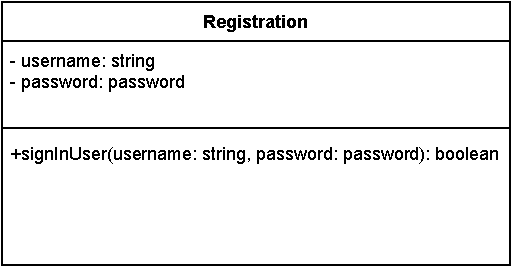
\includegraphics[scale=1]{res/Klassen/RegistrationClass.pdf}}
\caption{Registration class from class diagram}
\end{figure}

This class is used to sign up new Users for our application and also for airflow.


\begin{methodenv}{Methods}

\method{signUser(username: String, password: password): boolean}

Method uses username and password to sign up new user and returns a boolean to confirm the registration

\smallPara{Parameters}
\begin{itemize}
	\item{username:}
	The preferred username
	\item{password:}
	The preferred password
\end{itemize}

\smallPara{Exceptions}
\begin{itemize}
	\item{UserExistsException}
	Gets thrown if the user trys to register with an already used username
\end{itemize}
\end{methodenv}



\class{User}

\begin{figure}[H]
\centerline{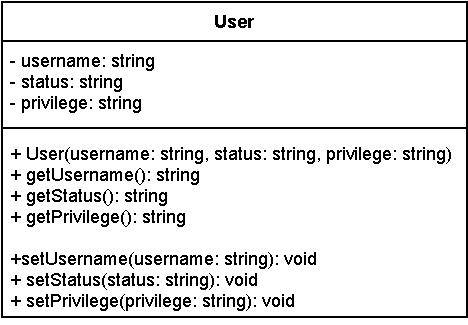
\includegraphics[scale=1]{res/Klassen/UserClass.pdf}}
\caption{User class from class diagram}
\end{figure}

This class is used to construct new Users.
\begin{methodenv}{Constructor}

\method{user(username: string, status: string, privilege: string)}

\smallPara{Parameters}

\begin{itemize}
	\item{username:}
	The users username
	\item{status:}
	The users status. Can be active, inactive or banned
	\item{privilege:}
	The users privilege. Can be Reviewer, Develloper or Admin
\end{itemize}
\end{methodenv}



\class{Login}

\begin{figure}[H]
\centerline{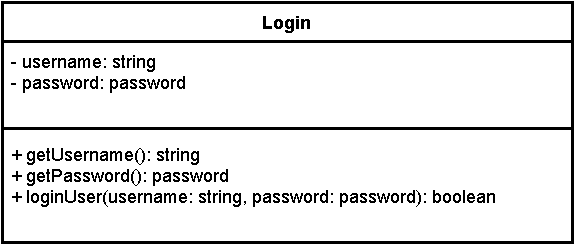
\includegraphics[scale=1]{res/Klassen/LoginClass.pdf}}
\caption{Login class from class diagram}
\end{figure}

This class is used to log in existing Users.

\begin{methodenv}{methods}

\method{loginUser(username: String, password: password): boolean}

Method uses username and password to log in user and returns a boolean to confirm the login.

\smallPara{Parameters}
\begin{itemize}
	\item{username:}
	The username to log in
	\item{password:}
	The password to log in
\end{itemize}
\end{methodenv}




\class{UserController}

\begin{figure}[H]
\centerline{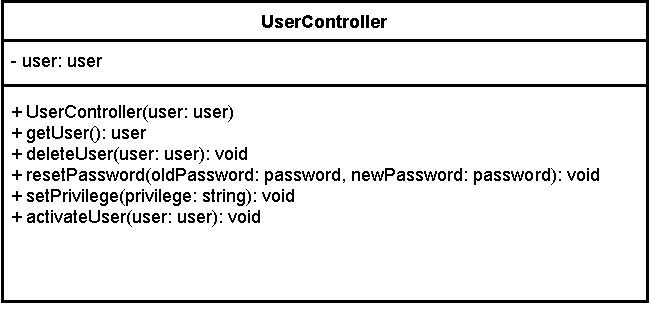
\includegraphics[scale=1]{res/Klassen/UserControllerClass.pdf}}
\caption{UserController class from class diagram}
\end{figure}

This class is used to change the parameters of existing users.

\begin{methodenv}{Constructor}

\method{UserController(user: user)}

\smallPara{Parameters}

\begin{itemize}
	\item{user:}
	The user that needs to be edited
\end{itemize}
\end{methodenv}

\begin{methodenv}{Methods}

\method{deleteUser(user:user): void}

Method gets the wanted User and deltes him. Afterwards the user is not able to log in anymore.

\smallPara{Parameters}
\begin{itemize}
	\item{user:}
	The user that is supposed to get deleted
\end{itemize}


\method{resetPassword(oldPassword: password, newPassword: password): void}

Method resets the users password and sets the new password.

\smallPara{Parameters}
\begin{itemize}
	\item{oldPassword:}
	The users old password that gets deleted
	\item{newPassword:}
	The users new password that is getting set
\end{itemize}

\method{setPrivilege(privilege: string): void}

Method resets the users old privilege and updates to the new privilege.

\smallPara{Parameters}
\begin{itemize}
	\item{privilege:}
	The privilege the user gets updated to
\end{itemize}

\method{activateUser(): void}

Method activates the User. The User can now log in to the application.

\end{methodenv}

\newpage









\subsubsection{Hardware Administration}
This package defines the logic behind the Hardware Administration.


\class{HardwareController}

\begin{figure}[H]
\centerline{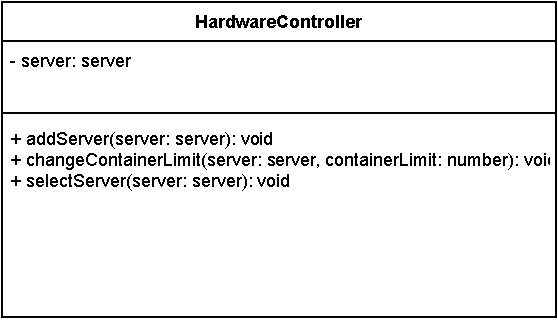
\includegraphics[scale=1]{res/Klassen/HardwareControllerClass.pdf}}
\caption{HardwareController class from class diagram}
\end{figure}

This class is used to surveillance and edit the Hardware of the Server

\begin{methodenv}{Methods}

\method{addServer(server: server): void}

Method adds a Server to the HardwareAdministration

\smallPara{Parameters}
\begin{itemize}
	\item{server:}
	The server that is getting added
\end{itemize}


\method{changeContainerLimit(server: server, containerLimit: number): void}

Method changes the containerlimit of the chosen server to the preferred number.

\smallPara{Parameters}
\begin{itemize}
	\item{server:}
	The server that is getting edited
	\item{containerLimit:}
	the number to which the containerlimit is getting updated to
\end{itemize}


\method{selectServer(server: server): void}

Method selects the server that is getting edited

\smallPara{Parameters}
\begin{itemize}
	\item{server:}
	The server that is getting selected
\end{itemize}
\end{methodenv}




\class{ Server}

\begin{figure}[H]
\centerline{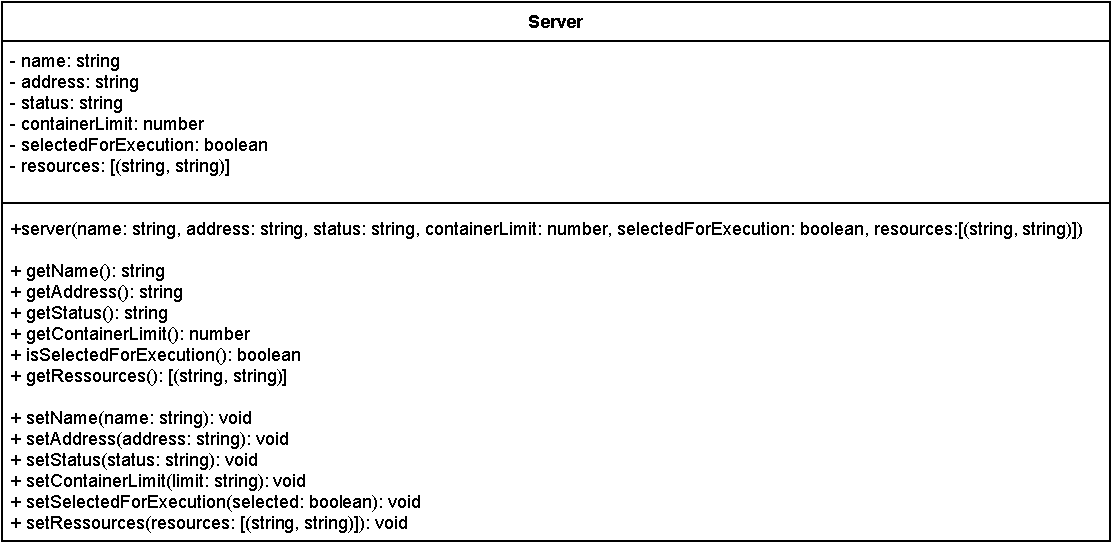
\includegraphics[scale=1]{res/Klassen/ServerClass.pdf}}
\caption{Server class from class diagram}
\end{figure}

This class is used to create a Server object

\begin{methodenv}{Constructor}

\method{server(name: string, address: string, status: string, containerLimit: number, selectedForExecution: boolean, resources: [(string, string)])}

\smallPara{Parameters}

\begin{itemize}
	\item{name:}
	The name of the server
	\item{address:}
	The serveraddress
	\item{status:}
	The server status
	\item{containerLimit:}
	The maximum of containers on the server
	\item{selectedForExecution:}
	Defines if the server is getting used or not
	\item{resources:}
	The servers resources
\end{itemize}
\end{methodenv}


\subsubsection{Database}

\subsubsection{WorkflowData}
Diese Klasse ist die Schnittstelle für alle Klassen die auf den Datenbankeinträgen für Workflows arbeiten wollen. Sie erstellt für jeden Zugriff den passenden Datenbankbefehl und konvertiert die Ergebnisse in das gewünschte Format des Aufrufers.
Sie wirft bei fehlerhaften Werten eine \textbf{MatFlowException}.

Diese Klasse, sowie alle anderen im Paket Database, ist nach dem Singleton Entwurfsmuster entworfen, da so Aufträge an die Datenbank so zentriert gesendet werden können.

\paragraph{createWorkflowInstanceFromTemplate(tName: String, wfName: String, confFold: Folder):void}
Create a new instance of a workflow by using the dag-file of a Template, 
with the Version set to 1. 
Search confDirect for every .conf-file and add them into the Database.
Set this Version as active Version.
\begin{itemize}
	\item \textbf{tName}
	name of Template of which the dag should be taken from
	\item \textbf{wfName}
	name of the new Workflow
	\item \textbf{confFold}
	the folder where all data of the Workflow is saved into
\end{itemize}


\paragraph{getNamesOfWorkflowsAndConfigFiles():String[][]]}
Return all Workflow names and the names of their corresponding config files.
The returning value is a list of lists of Strings where an inner list has the form [<Workflow Name>, <config File1 Name>, <config File2 Name>, ...]

\paragraph{createNewVersionOfWorkflowInstance(wfName:String, newVersion:DatabaseVersion, oldVersionNr:String):void}
Create a new Version of an existing Workflow with changed config Files.
Search which config Files changed and set those in the new Version.
\begin{itemize}
	\item \textbf{wfName}
	name of the Workflow
	\item \textbf{newVerson}
	new Version identifier
	\item \textbf{oldVersionNr}
	identifier of Version the new one is based on
\end{itemize}

\paragraph{getDatabaseVersionsOfWorkflowInstance(wfName:String):DatabaseVersion[]}
 Return all Versions of a Workflow Instance as DatabaseVersion Objects in a list.
 Asks the Database for the data and constructs every Object.
\begin{itemize}
	\item \textbf{wfName}
	name of the Workflow
\end{itemize}

\paragraph{setActiveVersionThroughNumber(wfName:String, version:String):void}
Set the previous Version as inactive and a new Version as active
\begin{itemize}
	\item \textbf{wfName}
	name of the Workflow
	\item \textbf{version}
	version to be set active
\end{itemize}

\paragraph{getVersionNumbersOfWorkflowInstance(wfName:String):String[]}
Return a sortet list of Strings of all Versions of a Workflow.
\begin{itemize}
	\item \textbf{wfName}
	name of Workflow which versions should be listed
\end{itemize}



\subsubsection{TemplateData}
Diese Klasse ist die Schnittstelle für alle Klassen die auf den Datenbankeinträgen für Workflow\_Template arbeiten wollen. Sie erstellt für jeden Zugriff den passenden Datenbankbefehl und konvertiert die Ergebnisse in das gewünschte Format des Aufrufers.
Sie wirft bei fehlerhaften Werten eine \textbf{MatFlowException}.

Diese Klasse, sowie alle anderen im Paket Database, ist nach dem Singleton Entwurfsmuster entworfen, da so Aufträge an die Datenbank so zentriert gesendet werden können.

\paragraph{createTemplate(template:Template):void}
Read Values from template and convert them into a sql query.
Throw error if name already exists.
\begin{itemize}
	\item \textbf{template}
	Template object to convert
\end{itemize}

\paragraph{getTemplateNames():String[]}
Return a list of all existing Template names.
List is empty when no Template exists.

\paragraph{getTemplateByNames(name:String):Template}
Return Template that is asked for.
Throw error if Template doesn't exist.
\begin{itemize}
	\item \textbf{name}
	name/identifier of the wanted Template
\end{itemize}



\subsubsection{DatabaseTable}
DatabaseTable ist die einzige Klasse die direkt mit der Datenbank kommuniziert. Ihre Funktion ist hauptsächlich MySQL Befehle entgegennimmt, diese an die Datenbank weiterzugeben und die dadurch erhaltenen Antworten zurückgibt. Im Fall eines Fehlers, wie einem leeren Ergebnis oder eines ungültigen Befehls wird eine \textbf{MatFlowException} geworfen.

Diese Klasse, sowie alle anderen im Paket Database, ist nach dem Singleton Entwurfsmuster entworfen, da so Aufträge an die Datenbank so zentriert gesendet werden können.

\paragraph{set(create: String):String} Create new entry on Database. Try to execute create on Database and return value.
\begin{itemize}
	\item \textbf{create} 
	a sql query to create an entry
\end{itemize}

\paragraph{delete(del: String):String} Delete an existing entry. Try to execute del on Database and return value.
\begin{itemize}
	\item \textbf{del} 
	a sql query to delete an entry
\end{itemize}

\paragraph{modify(change: String):String} Modify an existing entry. Try to execute change on Database and return value.
\begin{itemize}
	\item \textbf{change} 
	a sql query to change values
\end{itemize}


\newpage
\subsubsection{Exception package}

\paragraph{Package: exceptionPackage}This package contains all MatFlowExceptions.

\class{Exception}

\begin{figure}[H]
        \centerline{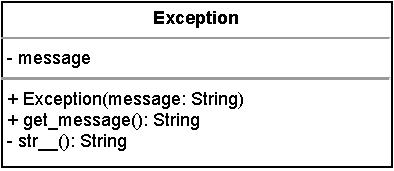
\includegraphics[scale=1]{res/Klassen/Exception.pdf}}
        \caption{Exception class from class diagram}
\end{figure}

This is the native Python exception package. See \url{https://docs.python.org/3/tutorial/errors.html} 
for more information on usage and best practices.

\class{MatFlowException}

\begin{figure}[H]
        \centerline{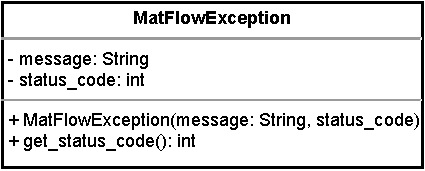
\includegraphics[scale=1]{res/Klassen/MatFlowException.pdf}}
        \caption{MatFlowException class from class diagram}
\end{figure}

This is the MatFlow parent exception from which all the specified exceptions inherit. It adds more functionality to 
a standard exception through the exception's status code and function which gets the status code. This is important for our
\nameref{API}.
\begin{methodenv}{Constructor}
\method{MatFlowException(message: String, status\texttt{\_}code: int): MatFlowException}
\smallPara{Parameters}
\begin{itemize}
	\item{message:}
	The message that is displayed when the exception is thrown. Native to the parent class but not relevant to application,
    nevertheless intriguing when extending this application 
    \item{status\texttt{\_}code:}
	The status code representing the thrown exception
\end{itemize}

\method{get\texttt{\_}status\texttt{\_}code(): int}
gets the status code

\end{methodenv}


\class{UserExistsException}

\begin{figure}[H]
        \centerline{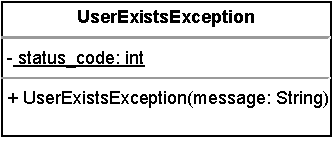
\includegraphics[scale=1]{res/Klassen/UserExistsException.pdf}}
        \caption{UserExistsException class from class diagram}
\end{figure}

This is an exception that is thrown when a user does not exist.
\begin{methodenv}{Constructor}

\method{UserExistsException(message : String)}
\smallPara{Parameters}
\begin{itemize}
    \item{message:}
    The message that is displayed when this exception is thrown.
\end{itemize}

\end{methodenv}

\class{DoubleTemplateNameException}

\begin{figure}[H]
    \centerline{\includegraphics[scale=1]{res/Klassen/DoubleTemplateNameException.pdf}}
    \caption{DoubleTemplateNameException class from class diagram}
\end{figure}

This is an exception that is thrown when the desired template name already exists.
\begin{methodenv}{Constructor}

\method{DoubleTemplateNameException(message : String)}
\smallPara{Parameters}
\begin{itemize}
    \item{message:}
    The message that is displayed when this exception is thrown.
\end{itemize}
\end{methodenv}


\class{InvalidDagFileException}

\begin{figure}[H]
    \centerline{\includegraphics[scale=1]{res/Klassen/InvalidDagFileException.pdf}}
    \caption{InvalidDagFileException class from class diagram}
\end{figure}

This is an exception that is thrown when the dag definition file is not correct (when dag file is finished coding).
\begin{methodenv}{Constructor}

\method{InvalidDagFileException(message : String)}
\smallPara{Parameters}
\begin{itemize}
    \item{message:}
    The message that is displayed when this exception is thrown.
\end{itemize}
\end{methodenv}


\class{DoubleWorkflowInstanceNameException}

\begin{figure}[H]
    \centerline{\includegraphics[scale=1]{res/Klassen/DoubleWorkflowInstanceNameException.pdf}}
    \caption{DoubleWorkflowInstanceNameException class from class diagram}
\end{figure}

This is an exception that is thrown when the desired workflow instance name already exists.
\begin{methodenv}{Constructor}

\method{DoubleWorkflowInstanceNameException(message : String)}
\smallPara{Parameters}
\begin{itemize}
    \item{message:}
    The message that is displayed when this exception is thrown.
\end{itemize}
\end{methodenv}


\class{EmptyConfigFolderException}

\begin{figure}[H]
    \centerline{\includegraphics[scale=1]{res/Klassen/EmptyConfigFolderException.pdf}}
    \caption{EmptyConfigFolderException class from class diagram}
\end{figure}

This is an exception that is thrown when the config folder is empty, meaning that no config can be selected.
\begin{methodenv}{Constructor}

\method{EmptyConfigFolderException(message : String)}
\smallPara{Parameters}
\begin{itemize}
    \item{message:}
    The message that is displayed when this exception is thrown.
\end{itemize}
\end{methodenv}


\class{WorkflowInstanceRunningException}

\begin{figure}[H]
    \centerline{\includegraphics[scale=1]{res/Klassen/WorkflowInstanceRunningException.pdf}}
    \caption{WorkflowInstanceRunningException class from class diagram}
\end{figure}

This is an exception that is thrown when the workflow instance is already running.
\begin{methodenv}{Constructor}

\method{WorkflowInstanceRunningException(message : String)}
\smallPara{Parameters}
\begin{itemize}
    \item{message:}
    The message that is displayed when this exception is thrown.
\end{itemize}
\end{methodenv}

\class{UnrepresentableDagException}

\begin{figure}[H]
    \centerline{\includegraphics[scale=1]{res/Klassen/UnrepresentableDagException.pdf}}
    \caption{UnrepresentableDagException class from class diagram}
\end{figure}

This is an exception that is thrown when the dag cannot be previewed(when dag file editing is in progress (JUST preview)).
\begin{methodenv}{Constructor}

\method{UnrepresentableDagException(message : String)}
\smallPara{Parameters}
\begin{itemize}
    \item{message:}
    The message that is displayed when this exception is thrown.
\end{itemize}
\end{methodenv}
\subsubsection{TGDS-Operator}
% Hier erstellt jeder eine eigene Datei und nennt sie <nameDesPakets>.tex und fügt sie anschließend mit
% "\input{<nameDesPakets>}" ein
% die erste Zeile in der Datei ist dann "\subsection{<nameDesPakets>}"

\newpage
\input{abläufe}
\section{Datenbank}

\subsection{Datenbankaufbau}
Die Datenbank beinhaltet folgende Tabellen:

\paragraph{}
\begin{dataTable}
	\hline
	\textbf{Workflow\_Template} &  & \\
	\hline
	name & String & $key; notNull$ \\
	\hline
	dag & .py -File & $notNull$\\
	\hline
\end{dataTable}

\paragraph{}
\begin{dataTable}
	\hline
	\textbf{Workflow} &  & \\
	\hline
	name & String & $key; notNull$ \\
	\hline
	files & String & $notNull$ \\
	\hline
	dag & .py  -File & $notNull$\\
	\hline
\end{dataTable}

\paragraph{}
\begin{dataTable}
	\hline
	\textbf{FolderFile} &  & \\
	\hline
	wfname & String & $key; notNull;$ name from Workflow\\
	\hline
	filesID & int & $key; notNull$ \\
	\hline
	file & File & $notNull$\\
	\hline
\end{dataTable}

\paragraph{}
\begin{dataTable}
	\hline
	\textbf{Version} & & \\
	\hline
	wfName & String & $key; notNull;$ name from Workflow\\
	\hline
	version & String & $key; notNull$ \\
	\hline
	note & String & \\
	\hline
\end{dataTable}

\paragraph{}
\begin{dataTable}
	\hline
	\textbf{ActiveVersion} & & \\
	\hline
	wfName & String & $key; notNull;$ name from Workflow\\
	\hline
	version & String & $notNull;$ from Version\\
	\hline
\end{dataTable}

\paragraph{}
\begin{dataTable}
	\hline
	\textbf{VersionFile} & & \\
	\hline
	wfName & String & $key; notNull;$ name from Workflow\\
	\hline
	version & String & $key; notNull;$ from Version \\
	\hline
	confKey & String & $key; notNull;$ from ConfFiles \\
	\hline
\end{dataTable}

\paragraph{}
\begin{dataTable}
	\hline
	\textbf{ConfFile} & & \\
	\hline
	confKey & String & $key; notNull$ \\
	\hline
	file & .conf -File & $notNull$ \\
	\hline
\end{dataTable}

\paragraph{}
\begin{dataTable}
	\hline
	\textbf{ResultFile} &  & \\
	\hline
	wfname & String & $key; notNull;$ name from Workflow\\
	\hline
	version & String & $key; notNull;$ from Version \\
	\hline
	filesID & int & $key; notNull$ \\
	\hline
	file & File & $notNull$\\
	\hline
\end{dataTable}

\paragraph{Anmerkung} Die dag Datei hätte als Schlüssel zwischen Workflow\_Template und Workflow fungieren können, ist aber redundant für alle Operationen auf einem Workflow.
Deshalb wurde entschieden die Datei bei einer Workflowerstellung direkt zu kopieren.


\newpage

% Glossar
\clearpage
%\printnoidxglossaries

\end{document}
